\documentclass[12pt,a4paper,openright,twoside]{book}

\usepackage[utf8]{inputenc}
\usepackage{float}
\usepackage{disi-thesis}
\usepackage{code-lstlistings}
\usepackage{notes}
\usepackage{shortcuts}
\usepackage{acronym}

\hypersetup{
    hidelinks % Nasconde i cerchiati attorno ai link
}


\school{\unibo}
\programme{Corso di Laurea Magistrale in Ingegneria e Scienze Informatiche}
\title{Identificazione umana mediante analisi di immagini radiografiche dentali\\
    \large per applicazioni in ambito forense
}
\author{Arianna Soriani}
\date{\today}
\subject{Visione Artificiale}
\supervisor{Prof.ssa Annalisa Franco}
\cosupervisor{Prof. Guido Borghi}
\session{III}
\academicyear{2023-2024}

% Definition of acronyms
%\acrodef{IoT}{Internet of Thing}
%\acrodef{vm}[VM]{Virtual Machine}


\mainlinespacing{1.241} % line spacing in mainmatter, comment to default (1)

\begin{document}

\frontmatter\frontispiece

\begin{abstract}	
Il progetto presentato nasce da una stretta collaborazione tra il Dipartimento di {\itshape Ingegneria e Scienze Informatiche} di Cesena e il Dipartimento dei {\itshape Beni Culturali} di Ravenna, in risposta alla necessità di sviluppare strumenti avanzati per l'analisi forense.\\

L’obiettivo del progetto consiste nello sviluppare un sistema che agevoli l’ identificazione di resti scheletrici attraverso l’{\itshape odontologia forense}, disciplina che sfrutta l’impronta dentale come metodo di riconoscimento.\\

I denti rappresentano uno tra i tessuti più resistenti e invarianti nel tempo; forniscono, dunque, un’efficace chiave identificativa, paragonabile, o persino superiore, ad altri metodi di riconoscimento, quali impronte digitali e DNA.\\

Il sistema progettato utilizza tecniche avanzate di elaborazione delle immagini al fine di reallizare una soluzione intelligente che confronti immagini radiografiche dentali acquisite al momento dell'analisi, con immagini preesistenti, memorizzate all'interno di un dataset odontologico.\\

Il progetto si pone l'obiettivo di realizzare una soluzione che fornisca ai ricercatori di Ravenna uno strumento intelligente e rapido per identificare scheletri, ampliando ed accelerando il processo di identificazione di resti, appartenenti ad epoche passate.
\end{abstract}

\begin{dedication} % this is optional
Optional. Max a few lines.
\end{dedication}

%----------------------------------------------------------------------------------------
\tableofcontents   
\listoffigures     % (optional) comment if empty
\lstlistoflistings % (optional) comment if empty
%----------------------------------------------------------------------------------------

\mainmatter

%----------------------------------------------------------------------------------------
\chapter{Introduzione}
\label{chap:introduction}
%----------------------------------------------------------------------------------------

Il progetto nasce da una stretta collaborazione tra il {\itshape Dipartimento di Ingegneria e Scienze Informatiche} di Cesena e il {\itshape Dipartimento dei Beni Culturali} di Ravenna. Questa iniziativa risponde a una specifica necessità del gruppo di ricerca interno al Dipartimento di Ravenna per applicazioni di analisi forense.\\

Insieme a metodi consolidati come {\itshape impronte digitali} e {\itshape Dna}, i denti rappresentano uno strumento fondamentale per l'identificazione personale; infatti, l’impronta dentale può risultare tanto efficace, se non più, di altri mezzi di riconoscimento.\\

Il termine {\itshape Odontologia forense} comprende tutte le attività di antropologia forense peculiari dell’odontoiatria e trova applicazioni in vari ambiti, tra cui assume particolare rilevanza quello dell'{\itshape identificazione personale}. L’odontologo forense, avvalendosi della documentazione ante-mortem, può ottenere risultati di elevata precisione.\\

I denti cosituiscono, infatti, il tessuto più resistente dell’organismo umano e mantengono la loro morfologia invariata, eccetto in casi di usura, decalcificazione o fratture. Per questo motivo, l’odontologia forense assume una particolare importanza nel contesto dell’identificazione di resti scheletrizzati o in stato di decomposizione avanzata.\\

Il Dipartimento dei Beni Culturali di Ravenna, in via sperimentale, conduce indagini su resti di corpi umani appartenenti a epoche storiche di cui rimangono solo pochi reperti scheletrici, con l’obiettivo primario di identificarli. La collaborazione con il Dipartimento di Ingegneria e Scienze Informatiche di Cesena è finalizzata proprio allo sviluppo di strumenti idonei a supportare tali attività.\\

L'obiettivo del progetto è, dunque, realizzare un sistema avanzato che consenta ai ricercatori di Ravenna di identificare, in modo efficiente ed intelligente, resti scheletrici tramite l'impronta dentale. Il sistema sarà in grado di confrontare immagini radiografiche dentali acquisite durante l’analisi, con immagini presenti in un dataset specifico contenente documentazione odontologica preesistente, agevolando, facilitando e accelerando così il processo di identificazione.

%\sidenote{Add sidenotes in this way. They are named after the author of the thesis}

\chapter{Analisi dei dati}

\section{Struttura del dataset}
Il {\itshape Dipartimento dei Beni Culturali} di Ravenna, dalla cui collaborazione è nata l'idea del progetto, ha fornito, in forma totalmente anonima, un dataset contenente le immagini radiografiche da loro possedute; ogni radiografia si riferisce ad un corpo finalizzato allo studio di analisi forense. \\
Il dataset fornito contiene immagini relative a 100 pazienti anonimi.\\
Il {\itshape dataset}, per come è stato fornito, è suddiviso in subdirectory, ciascuna contenente la documentazione relativa ad un singolo paziente. Ogni persona è identificata attraverso un valore numerico, intero, crescente e unico(es. "P\_5"). \\
Ogni subdirectory presenta la medesima struttura: 
\begin{itemize}
\item Nome subdirectory: {\itshape P\_idNumber}
\item 4 immagini radiografiche
\end{itemize}
%\begin{figure}
  %  \centering
   % 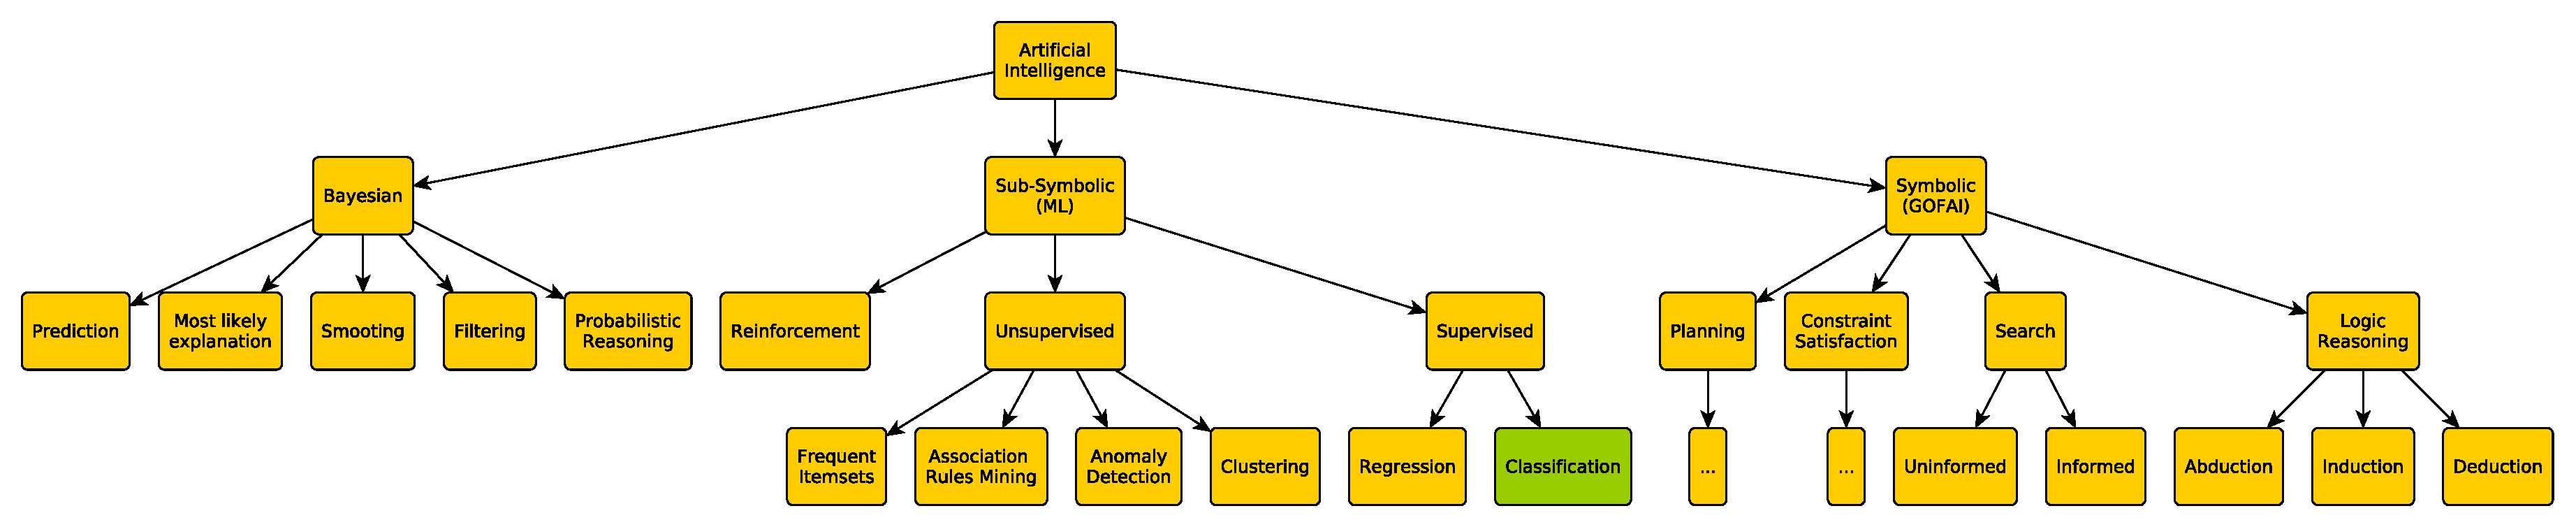
\includegraphics[width=.8\linewidth]{figures/random-image.pdf}
   % \caption{Some random image}
   % \label{fig:random-image}
%\end{figure}
\newpage
\begin{figure}[H]
    \centering
    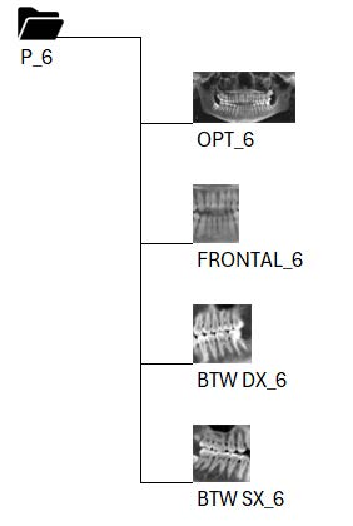
\includegraphics[height=7cm,width=5cm]{figures/subdir.pdf}
    \caption{Subdirectory}
    \label{fig:subdirectory}
\end{figure}

Il formato desiderato per ogni immagine memorizzata è il seguente:
\begin{itemize}
\item \textbf{OTP\_idNumber}: radiografia ortopanoramica.
\item \textbf{FRONTAL\_idNumber}: radiografia di bitewing frontale.
\item \textbf{BTW SX\_idNumber}: radiografia di bitewing della porzione sinistra dell'ortopanoramica.
\item \textbf{BTW DX\_idNumber}: radiografia di bitewing della porzione destra dell'ortopanoramica.
\end{itemize}

\begin{figure}[H]
    \centering
    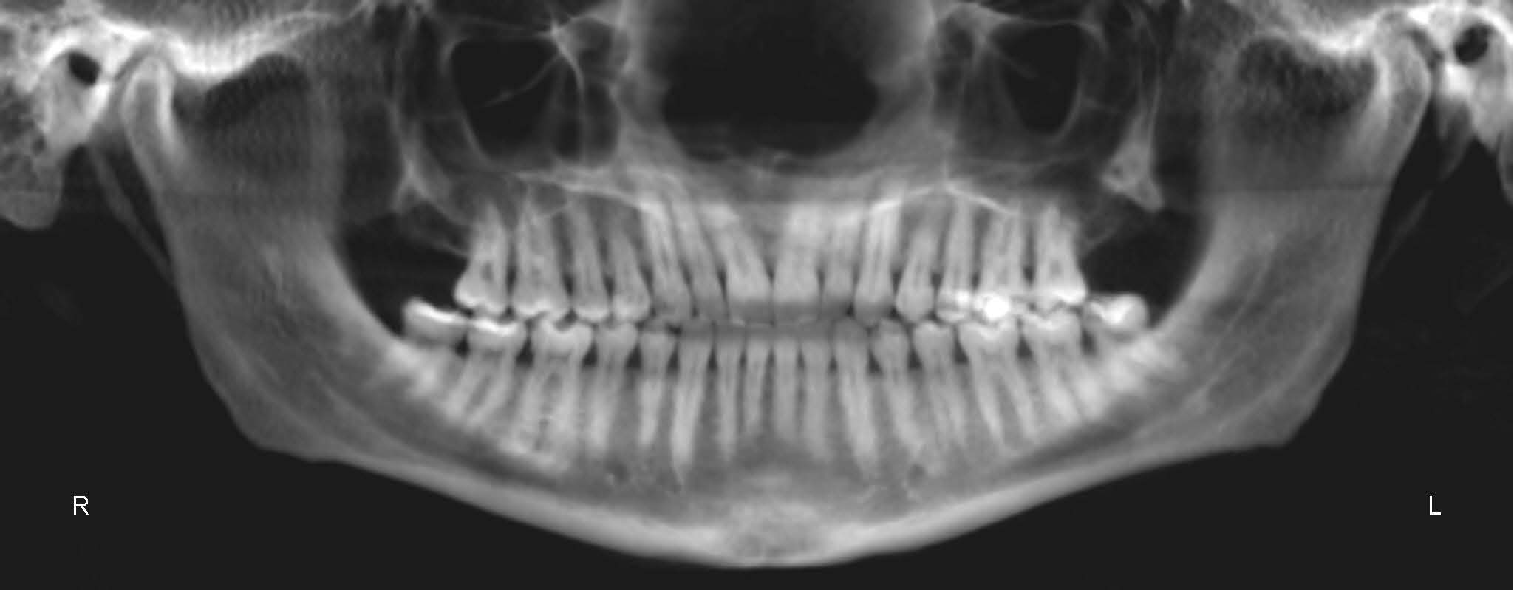
\includegraphics[width=8cm]{figures/opt.pdf}
    \caption{Ortopanoramica}
    \label{fig:opt}
\end{figure}
\begin{figure}[H]
    \centering
    \begin{minipage}{0.3\textwidth}
	\centering
    	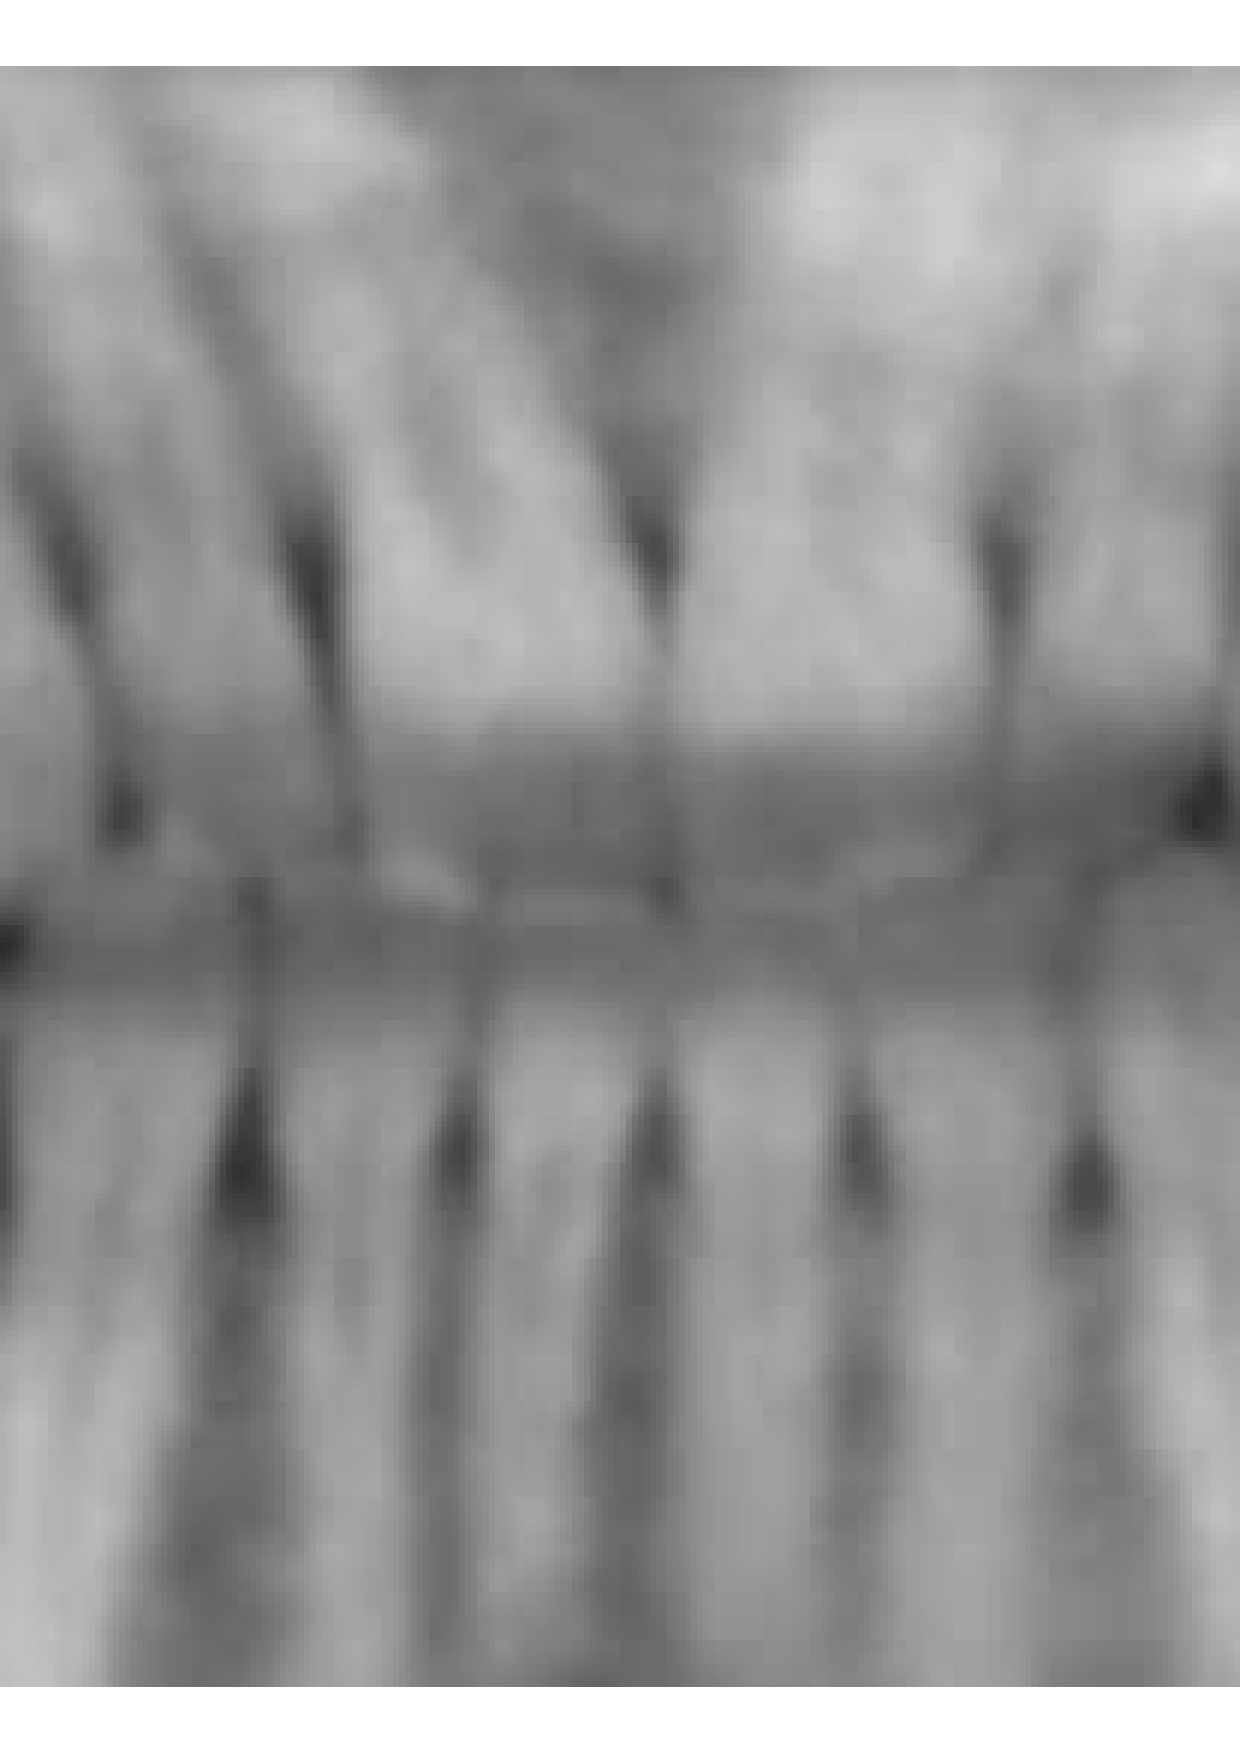
\includegraphics[height=4cm,width=3cm]{figures/FRONTAL.pdf}
    	\caption{Bitewing frontale}
    	\label{lab:Bitewing frontale}
    \end{minipage}\hfill
    \begin{minipage}{0.3\textwidth}
    	\centering
    	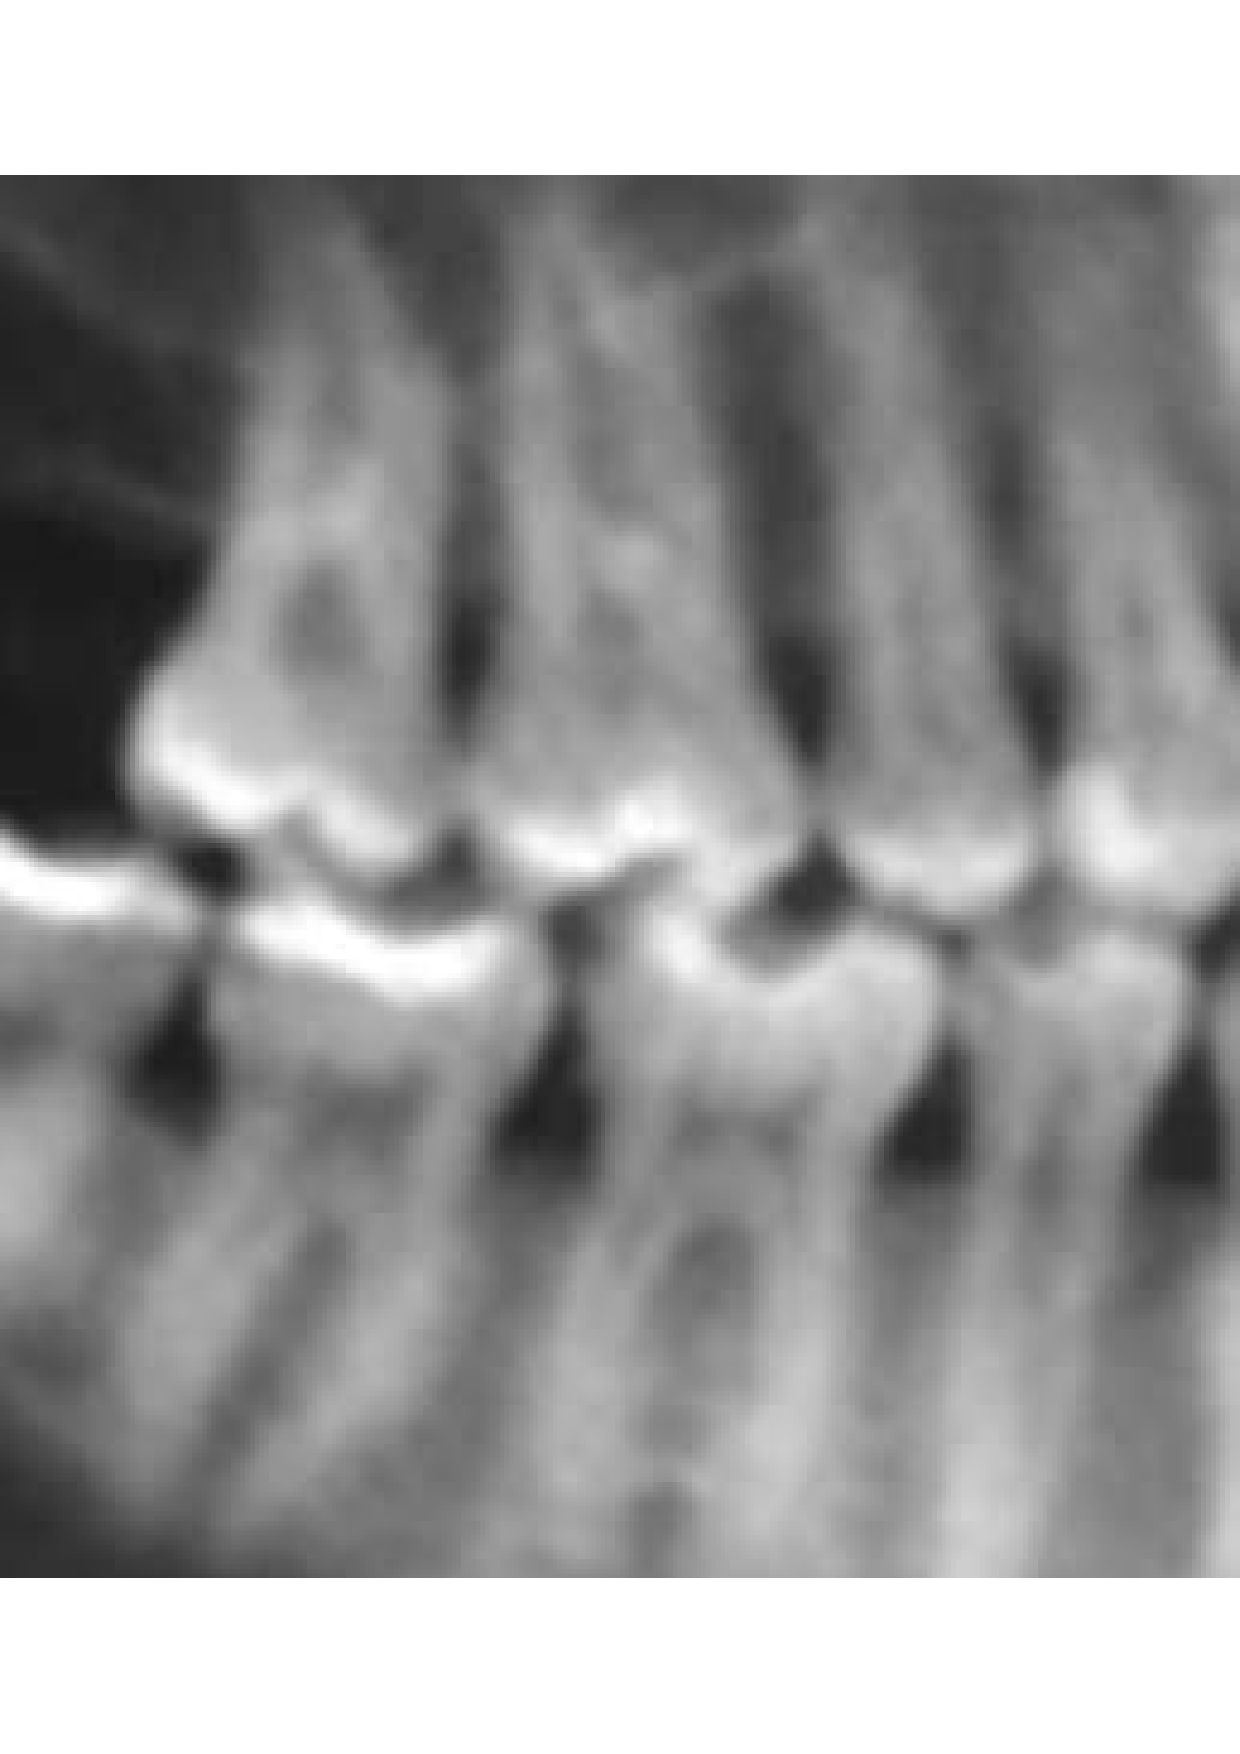
\includegraphics[height=4cm,width=3cm]{figures/BTWSX.pdf}
    	\caption{Bitewing sinistro}
    	\label{lab:Bitewing sinistro}
    \end{minipage}\hfill
    \begin{minipage}{0.3\textwidth}
    	\centering
    	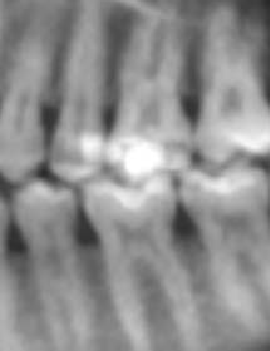
\includegraphics[height=4cm,width=3cm]{figures/BTWDX.pdf}
    	\caption{Bitewing destro}
   	\label{lab:Bitewing destro}
    \end{minipage}
\end{figure}

%%%%%%%%%%%%%%%%%%%%%%%%%%%%%%%%%%%%%%%%%%%%%%%%%%%
\section{Studio preliminare}
Da una prima analisi effettuata sul dataset, emerge immediatamente la non uniformità dei dati. Molte immagini, infatti, non ottemperano al pattern di struttura definito nella sezione precedente. I dati, così forniti, non sono sfruttabili per applicazioni intelligenti di Visione Artificiale.\\
Al fine di effettuare uno studio preliminare di analisi dei dati, sono state mantenute {\itshape solo} le subdirectory le cui immagini risultassero conformi alla struttura dei dati richiesta.\\

\subsection{Suddivisione del dataset}
Il dataset utilizzato nella fase preliminare, è definito come un sottoinsieme dell'insieme di partenza; composto unicamente dal range di pazienti 61-100. Infatti, solo questi pazienti presentano, in una prima analisi, un formato conforme dei dati. Questo a giustificazione del fatto, che i dati risalgono a periodi di acquisizione diversi e a modalità di acquisizione diverse; solo per questo sottoinsieme è posssibile garantire una nomenclatura corretta delle immagini, un formato conforme al pattern definito e un insieme di immagini "pulite" in termini di: luminosità, distorsione, rotazione, prospettiva, dimensione e proporzione.

\subsection{Idea}
Al fine di realizzare uno studio preliminare sui dati, vengono definiti e implementati alcuni algoritmi di \textbf{Feature Detection e Matching}.\\
Questi algoritmi seguono i seguenti passaggi:
\begin{enumerate}
\item Estrazione dei \textbf{keypoint} dalle immagini ortopanoramiche (OPT).
\item Estrazione dei \textbf{keypoint} dalle immagini parziali di bitewing (FRONTAL e BTW).
\item Matching tra i \textbf{descrittori} dei keypoint individuati negli step precedenti.
\end{enumerate}

%%%%%%%%%%%%%%%%%%%%%%%%%%%%%%%%%%%%%%%%
\chapter{Tipologie di Matching}
Il processo di \textbf{Feature Detection e Matching} è un task molto importante di molte applicazioni di Computer Vision come: structure-from-motion, image retrieval, object detection, ecc. Essa consiste in una tecnica fondamentale che prevede l'identificazione e l'allineamento di feature corrispondenti in più immagini.\\
Le \textbf{feature} si riferiscono a elementi distintivi di un'immagine, come  {\itshape bordi, angoli o blob}, che possono essere rilevati e descritti in modo consistente. Attraverso il matching tra feature, appartenenti a immagini distinte, i sistemi di Computer Vision sono in grado di riconoscere oggetti, tracciare movimenti, creare immagini panoramiche o ricostruire scene 3D da immagini 2D.\\

Gli aspetti chiave del Feature Matching sono:
\begin{enumerate}

\item \textbf{Feature Detection}\\
Il processo inizia con il rilevamento delle key features all'interno di ogni immagine. Queste feature sono tipicamente punti di interesse facili da distinguere, come angoli o bordi. Esistono diversi  sistemi di detection molto avanzati, come {\itshape Harris Corner Detector} o {\itshape Laplacian of Gaussian for blob detection}.

\item \textbf{Feature Description}\\
Una volta individuate le feature, esse vengono descritte attraverso dei \textbf{feature descriptors}, i quali forniscono una rappresentazione numerica delle caratteristiche della feature. I descrittori più diffusi sono {\itshape SIFT} (Scale-Invariant Feature Transform), {\itshape SURF} (Speeded Up Robust Features), ORB (Oriented FAST and Rotated BRIEF) e {\itshape BRIEF} (Binary Robust Independent Elementary Features).

\item \textbf{Feature Matching}\\
Lo step core consiste nel confrontare i descrittori di feature, appartenenti a immagini diverse, al fine di individuare le corrispondenze esistenti. \\
Vengono comunemente utilizzate tecniche come: {\itshape brute-force matching}, in cui ogni feature viene confrontata con tutte le feature della seconda immagine, o il  {\itshape K-Nearest Neighbors (KNN) matching}, in cui vengono identificate le K corrispondenze più vicine.\\
Metodi di matching più robusti, quali {\itshape RANSAC} (Random Sample Consensus) aiutano a ridurre il rumore e la presenza di outlier, al fine di migliorare l'accuracy del sistema.

\end{enumerate}

\subsection{Feature Description}
L'operazione di {\itshape feature description} è uno step cruciale nel processo di feature matching, dove le feature individuate vengono rappresentate in una modalità tale da consentirne il confronto e il match rispetto a immagini differenti.\\
I descrittori di feature forniscono una {\itshape rappresentazione numerica o simbolica} delle caratteristiche delle features, consentendo un'efficace identificazione e allineamento tra feature corrispondenti.\\
I feature descriptors catturano l'aspetto locale intorno ad una feature, in maniera \textbf{invariante} rispetto a diverse operazioni di trasformazione, quali scala, rotazione o cambiamenti di illuminazione a seconda di come essi vengono definiti.\\
Essi trasformano i valori dei pixel in prossimità della feature in un {\itshape vettore compatto} e di {\itshape lunghezza definita} che identifica in maniera univoca la feature individuata.\\
Questo vettore può essere, poi, utilizzato per confrontare e abbinare le feature tra le diverse immagini.\\
I feature descriptors più conosciuti e utilizzati sono:
\begin{enumerate}

\item \textbf{SIFT (Scale-Invariant Feature Transform)}\\
SIFT genera un descrittore indipendente dalla scala e dalla rotazione; si occupa di identificare i keypoint dell'immagine a varie scale e orientamenti. Ogni keypoint è descritto da un vettore di 128 dimensioni che cattura la distribuzione dell'orientamento del gradiente intorno al keypoint.

\item \textbf{SURF (Speeded Up Robust Features)}\\
SURF è un'alternativa efficiente a SIFT, che utilizza un'immagine integrale per un calcolo più veloce dei vettori. Produce un descrittore robusto alla scala e alla rotazione, ma può essere calcolato più rapidamente rispetto a SIFT.

\item \textbf{ORB (Oriented FAST and Rotated BRIEF)}\\
ORB combina il keypoint detector FAST con il descrittore BRIEF. Fornisce un descrittore binario che risulta efficiente da calcolare e da abbinare, il chè lo rende adatto ad ambienti con risorse limitate. ORB include anche l'invarianza di orientamento, calcolando l'orientamento di ciascun keypoint.

\item \textbf{BRIEF (Binary Robust Independent Elementary Features)}\\
BRIEF genera una stringa binaria confrontando le intensità di coppie di pixel intorno a un keypoint. È molto efficiente sia in termini di calcolo che in termini di memorizzazione, ma manca di robustezza ai cambiamenti di scala e di rotazione.
\end{enumerate}

%%%%%%%%%%%%%%%%%%%%%%%%%%%%%%%%%%%%%%%%%%%%
\subsection{Feature Matching}
L'operazione di {\itshape feature matching} comporta il confronto dei descrittori di feature allo scopo di individuare feature corrispondenti in immagini diverse. \\
Per garantire una corrispondenza accurata ed efficiente, vengono impiegate diverse tecniche, tra cui:

\begin{enumerate}

\item \textbf{Keypoint Matching}\\
Il Keypoint Matching è il processo di ricerca dei keypoint corrispondenti, tra immagini diverse, attraverso il confronto dei loro descrittori. L'obiettivo è identificare coppie di punti chiave che rappresentano lo stesso punto fisico nella scena.

\item \textbf{Brute-Force Matcher}\\
Il Brute-Force Matcher confronta ogni descrittore di un'immagine con ogni descrittore di un'altra immagine per trovare le migliori corrispondenze in base a una metrica di distanza scelta (ad esempio, la distanza euclidea).
\begin{itemize}
\item {\itshape Vantaggi}: Semplice e diretto, fornisce corrispondenze accurate.
\item {\itshape Svantaggi}: Costoso dal punto di vista computazionale, soprattutto per grandi insiemi di dati.
\end{itemize}

\item \textbf{K-Nearest Neighbors (KNN) Matching}\\
Il K-Nearest Neighbors Matching trova i k descrittori più vicini per ogni keypoint in base ad una metrica di distanza. In genere, si applica il \textbf{ratio test} per selezionare la migliore corrispondenza tra i k vicini.
\begin{itemize}
\item {\itshape Vantaggi}: Più efficiente della corrispondenza brute-force, consente una certa flessibilità nella selezione della corrispondenza migliore.
\item {\itshape Svantaggi}: Ancora intensivo dal punto di vista computazionale per insiemi di dati molto grandi.
\end{itemize}

\item \textbf{RANSAC (Random Sample Consensus)}\\
Per Robust Matching, RANSAC è un metodo iterativo utilizzato per stimare i parametri di un modello matematico da un insieme di dati osservati che contengono outlier. Nel feature matching, RANSAC viene utilizzato per trovare un insieme robusto di corrispondenze selezionando ripetutamente sottoinsiemi casuali di corrispondenze e calcolando una trasformazione che allinei le immagini. Viene scelta la trasformazione con il maggior numero di valori anomali.
\begin{itemize}
\item {\itshape Vantaggi}: Robustezza agli outlier e al rumore, migliora l'accuratezza del feature matching.
\item {\itshape Svantaggi}:  Intenso dal punto di vista computazionale, richiede un'attenta regolazione dei parametri.
\end{itemize}

\end{enumerate}

%%%%%%%%%%%%%%%%%%%%%%%%%%%%%%%%%%%%%%%%%%%%
\subsection{Template Matching}
Nell'analisi preliminare, viene analizzato l'insieme di dati anche attraverso l'ausilio di un secondo metodo di Matching molto conosciuto, denominato \textbf{Template Matching}.\\
Il Template Matching è una tecnica di alto livello, utilizzata in applicazioni di Computer Vision, al fine di individuare la posizione, o le posizioni, di un certo template fornito come immagine, all'interno di un'altra immagine più grande.\\
Esistono diversi algoritmi di template matching avanzati che permettono di individuare le occorrenze del template indipendentemente dall'orientamento o dalla luminosità locale.\\
Le tecniche di Template Matching sono flessibili e relativamente semplici da usare, il chè le rende uno dei metodi più popolari nei compiti di Object Detection.\\
La loro applicabilità è limitata soprattutto dalla potenza di calcolo disponibile, poiché l'identificazione di modelli grandi e complessi può richiedere molto tempo.\\

L'obiettivo di questo modello è quello di individuare tutte le occorrenze e posizioni di un'immagine di riferimento (template) all'interno di un'altra immagine (immagine di input), indipendentemente dalla scala o dalla rotazione.\\

Il modello utilizzato è  \textbf{TM\_CCOEFF\_NORMED}, il quale lavora sull'intera immagine di query (OPT) e ricerca le occorrenze dell'immagine di bitewing fornita (BTW o FRONTAL). E' un modello molto semplice e veloce.\\
Quest'ultimo, calcola una matrice di matching come sovrapposizione rispetto all'immagine intera e determina i punti in cui si sovrappone meglio.

%%%%%%%%%%%%%%%%%%%%%%%%%%%%5
\chapter{Analisi Preliminare}
Al fine di realizzare una prima analisi dei dati, in particolare sul sottoinsieme del dataset di partenza (P61-P100), viene implementato un sistema di valutazione e di identificazione di immagini. Vengono implementati due algoritmi: uno per il feature matching e il secondo per il template matching.\\
Il primo processo segue diversi passi computazionali che possono essere così rappresentati:
\begin{figure}[H]
	\centering
	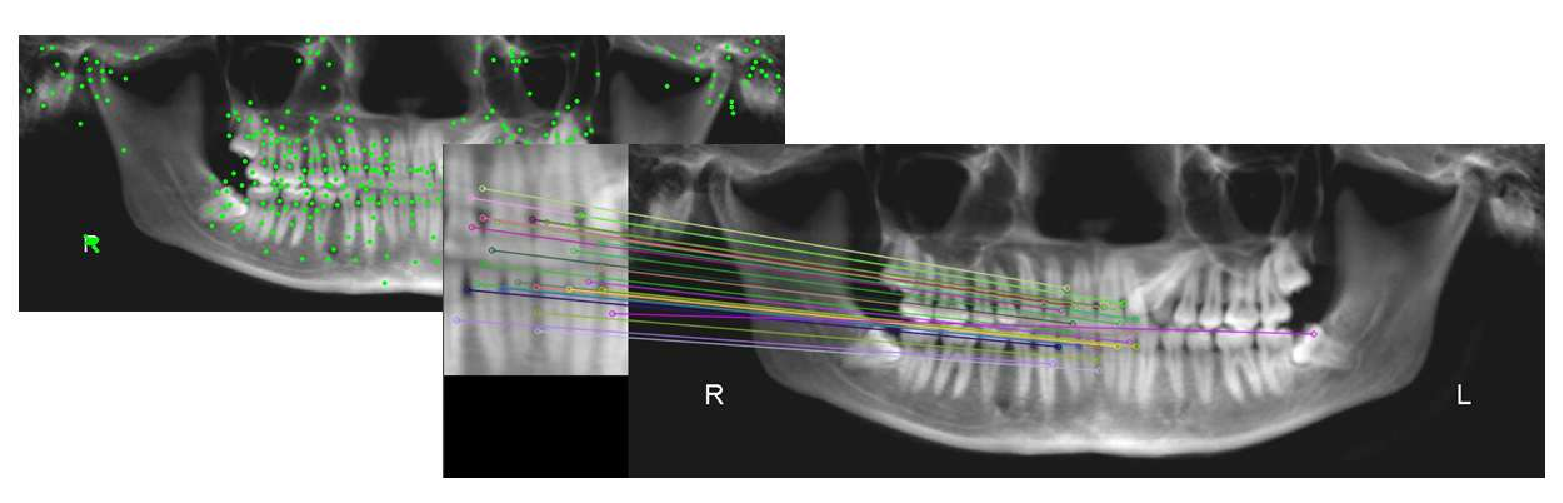
\includegraphics[height=6cm,width=16cm]{figures/keypoint.pdf}
    	\caption{Feature Descriptors e Feature Matching}
	\label{fig:keypointdescriptor}
\end{figure}
Ossia:
\begin{itemize}
\item Estrazione dei keypoint e definizione dei feature descriptor nelle immagini ortopanoramiche (OPT).
\item Estrazione dei keypoint e definizione dei feature descriptor nelle immagini parziali di bitewing (BTW e FRONTAL).
\item Feature Matching tra immagini ortopanoramiche e immagini di bitewing.
\item Identificazione e riconoscimento delle immagini parziali.
\end{itemize}

\begin{figure}[H]
	\centering
	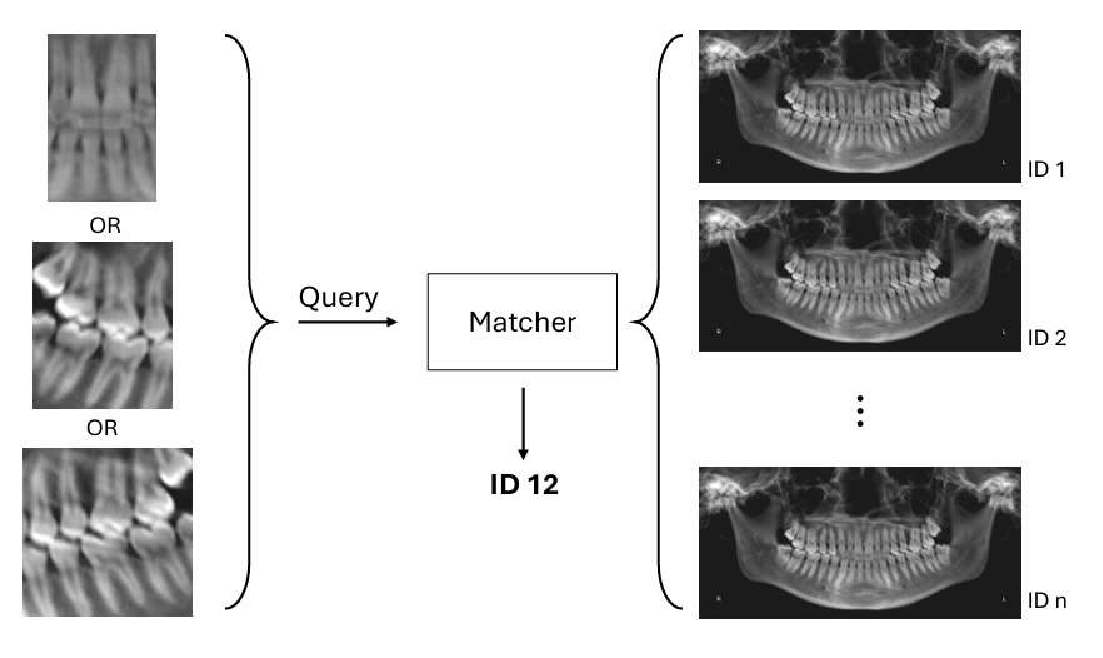
\includegraphics[height=6cm,width=11cm]{figures/matchprof.pdf}
    	\caption{Insieme di Feature Matching}
	\label{fig:featurematching}
\end{figure}


%%%%%%%%%%%%%%%%%%%%%%%%%%%%%%%%%%%%%5
\subsection{Protocollo operativo}
Lo schema di esecuzione dell'algoritmo di matching si basa sul confronto di una singola immagine di query, immagine di bitewing, con tutte le immagini ortopanoramiche presenti nel dataset, in questo caso 40.\\
Ai fini della valutazione dell'accuratezza del sistema, vengono studiate e analizzate tre metriche, definite come:
\begin{itemize}
\item \textbf{Rank@1}: il match corretto si trova nella prima posizione.
\item \textbf{Rank@2}: il match corretto si trova entro le prime due posizioni.
\item \textbf{Rank@5}: il match corretto si trova entro le prime cinque posizioni.
\end{itemize}

%%%%%%%%%%%%%%%%%%%%%%%%%%%%%%%%%%%%%5
\subsection{Risultati ottenuti}
I risultati ottenuti attraverso questa prima valutazione, sono molto buoni; essi, infatti, presentano valori altamente competitivi in termini di accuracy anche a livello di Rank@1.\\
Dal matching delle immagini di bitewing frontali (FRONTAL), i risultati ottenuti sono i seguenti:

\begin{figure}[H]
	\centering
	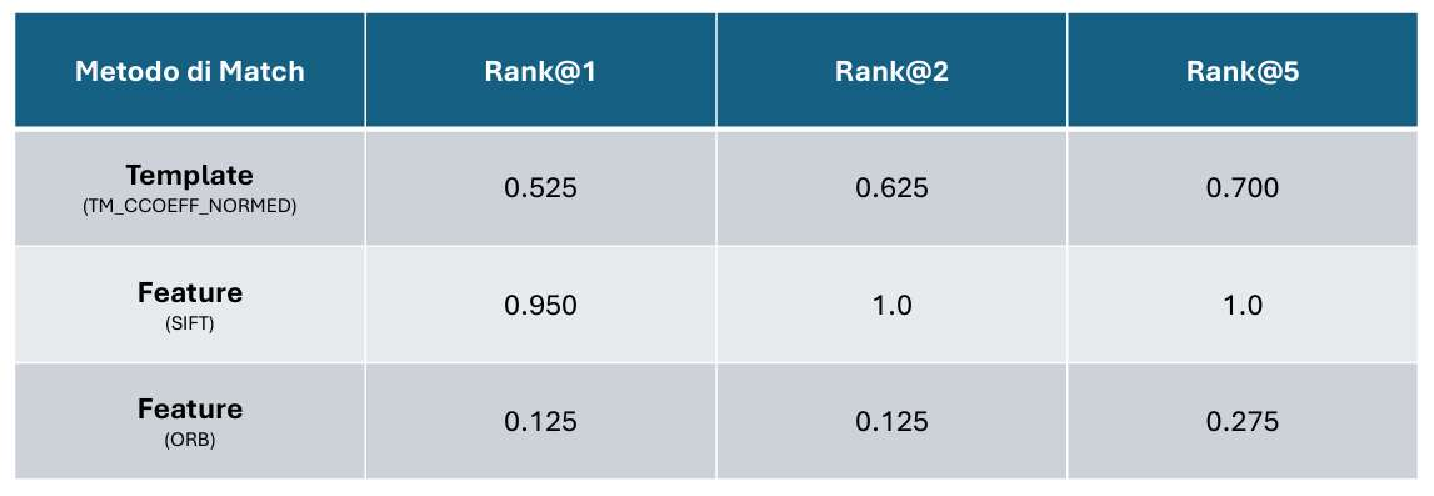
\includegraphics[height=5cm,width=15cm]{figures/frontalprof.pdf}
    	\caption{Matching delle immagini Frontal}
	\label{fig:frontalprof}
\end{figure}

Nella tabella sopra riportata, è possibile vedere l'ottimalità dei risultati ottenuti, soprattutto quando si utilizzano i keypoint SIFT, i quali, infatti, sono per definizione più precisi. \\
Dal match di immagini di Bitewing laterali, si ottengono, similmente, risultati molto buoni:
\begin{figure}[H]
	\centering
	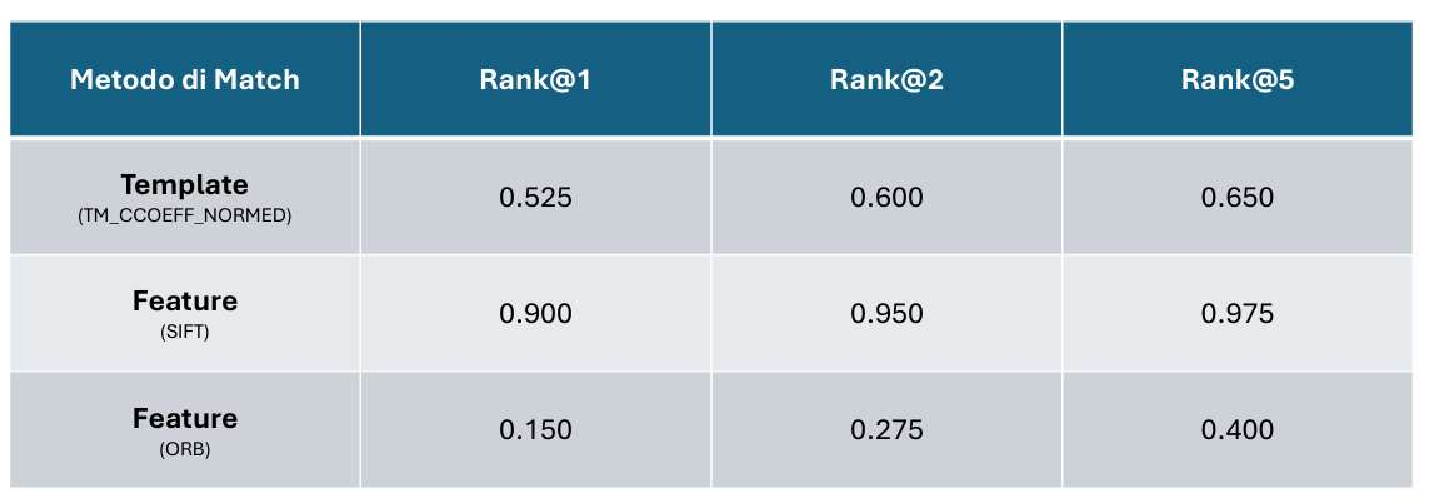
\includegraphics[height=5cm,width=15cm]{figures/dxprof.pdf}
    	\caption{Matching delle immagini BTW DX}
	\label{fig:dxprof}
\end{figure}
\begin{figure}[H]
	\centering
	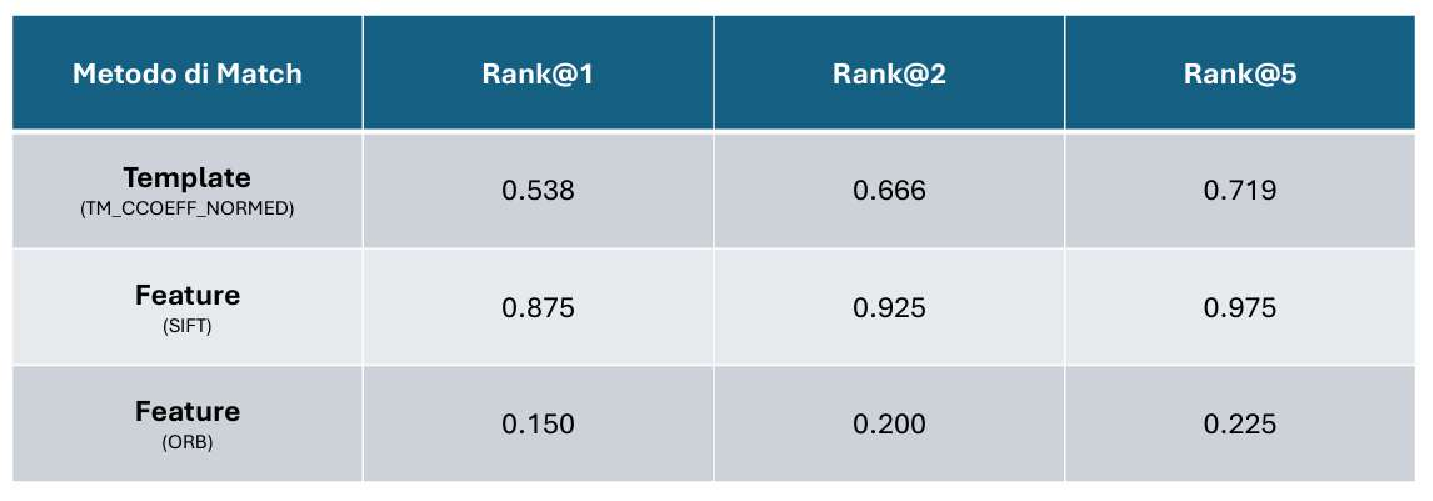
\includegraphics[height=5cm,width=15cm]{figures/sxprof.pdf}
    	\caption{Matching delle immagini BTW SX}
	\label{fig:sxprof}
\end{figure}

Dai risultati ottenuti dal match delle immagini laterali si può osservare come l'accuratezza decresca a causa del problema intrinseco legato alla tipologia delle immagini stesse, rispetto al cambiamento di prospettiva. Alcuni keypoint sono, però, robusti a fronte di questa tipologia di problema.\\
Un'ulteriore miglioria apportabile, potrebbe essere quella di definire dei meccanismi di supporto per gestire con questo tipo di problema. 

\subsection{Tempi di esecuzione}
I tempi di esecuzione ottenuti dai diversi algoritmi di matching sono i seguenti:
\begin{figure}[H]
	\centering
	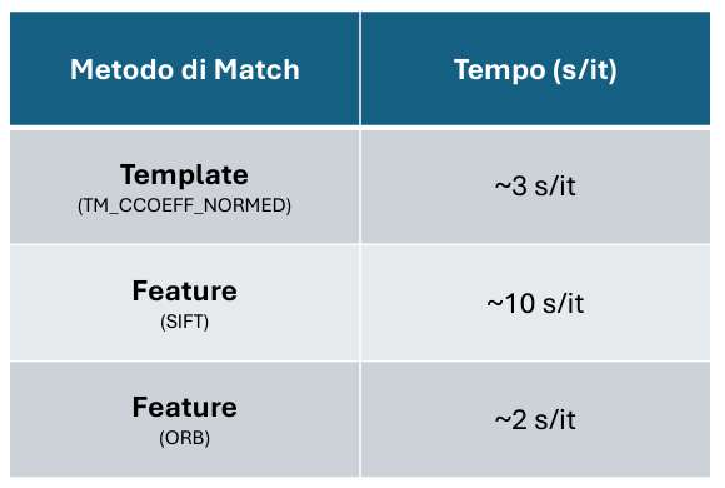
\includegraphics[height=5cm,width=7cm]{figures/tempiprof.pdf}
    	\caption{Tempi di esecuzione}
	\label{fig:tempiprof}
\end{figure}

Nonostante la dimensionalità molto bassa del database (solo 40 pazienti) i tempi di esecuzione richiesti non sono propriamente bassi; infatti, soprattutto con il keypoint SIFT è richiesto un tempo di processamento per ogni singolo match di circa 10s.\\
Feature ORB è il metodo di match con tempi di esecuzione più bassi, ma risultati di match peggiori.


%%%%%%%%%%%%%%%%%%%%%%%%%%%%%%%%%%%%%%%%%%%%%%%%%%%
\section{Problemi da affrontare}
Il progetto così strutturato, presenta diverse limitazioni, tra cui:
\begin{itemize}
\item Cardinalità del dataset troppo piccola: solo \textbf{40} immagini.
\item Immagini "perfette", non rappresentative della realtà.
\item Analisi effettuata solo attraverso due algoritmi di Feature Matching noti: SIFT e ORB.
\item Matching tra  immagini ortopanoramiche e di bitewing con rapporto 1:1 .
\item Feature Matching effettuato sull'intera immagine ortopanoramica.
\item Nessun raffinamento per il cambiamento di prospettiva per le immagini di Bitewing laterali.
\item Nessuna valutazione sul cambiamento nel tempo della confrormazione dell'impronta dentale, sistema non robusto.
\item Dataset  "semplice", non presenta alcun problema di scala
\end{itemize}
Dalle conclusioni ottenute dalla prima trattazione del problema, emerge che ogni soluzione proposta, presenta sia aspetti positivi, che aspetti negativi da trattare. In particolare:
\begin{itemize}
\item \textbf{ORB}: richiede un tempo di esecuzione minore, ma offre risultati di matching peggiori.
\item \textbf{Template Match}: richiede un tempo intermedio e offre risultati intermedi.
\item \textbf{SIFT}: notevolmente più lento, ma offre risultati molto migliori.
\end{itemize}
Nei seguenti step del progetto, viene affrontato il problema, allo scopo di realizzare una soluzione il più robusta, generale e applicabile possibile.


%%%%%%%%%%%%%%%%%%%%%%%%%%%%%%%%%%%%%%%%%%%
\chapter{Aumento della cardinalità del dataset}
Il {\itshape Dipartimento dei Beni Culturali} di Ravenna, dalla cui collaborazione è nata l'idea dello studio, ha fornito, in forma totalmente anonima, il dataset contenente le immagini radiografiche da loro posseduto; ogni radiografia si riferisce ad un corpo di analisi forense. \\
Il dataset fornito contiene immagini relative a 100 pazienti anonimi. Purtroppo, però, il dataset così presentato non è utilizzabile per uno studio in ambito di Visione Artificiale; gli algoritmi di questa disciplina richiedono formalismi e rigori che i dati, nativamente, non presentano.\\

Il primo studio, effettuato su questi dati, ha ristretto l'utilizzo delle immagini ai soli pazienti appartenenti alle subdirectory {\itshape 61-100}, poichè conformi al pattern strutturale desiderato.\\
Al fine di realizzare un sistema il più robusto e generico possibile, però, la cardinalità del dataset è incompatibile con la cardinalità richiesta dai sistemi di Computer Vision.\\
E' fondamentale, perciò, per una corretta realizzazione di un sistema robusto di {\itshape Human Tooth Identification}, accrescere il dataset per aumentarne la complessità, generalizzazione e applicabilità.\\
I passi presentati di seguito sono fondamentali al fine di ottemperare questo obiettivo.

%%%%%%%%%%%%%%%%%%%%%%%%%%%%%%%%%%%%%%%%%%%%%%%%%%%%%%%
\section{Il problema della cardinalità}
La cardinalità di un dataset, ovvero il numero di elementi unici e distinti presenti, ha un impatto significativo sull'applicabilità degli algoritmi di Computer Vision. Una bassa cardinalità può influenzare vari aspetti, come la capacità del modello di generalizzare, può portare il rischio di overfitting e può inficiare sulle prestazioni globali del sistema.\\
In particolare: 
\begin{itemize}
\item \textbf{Problemi di Overfitting}:\\
Quando si ha un dataset con bassa cardinalità, si rischia che il modello diventi troppo specifico per i dati di addestramento. Gli algoritmi di Deep Learning, in particolare, hanno una grande capacità di apprendimento e tendono a sovradimensionare le caratteristiche specifiche del dataset. Questo porta a problemi di {\itshape overfitting}, dove il modello performa molto bene sui dati di addestramento, ma male su dati nuovi o non visti.

\item \textbf{Generalizzazione limitata}:\\
Con una bassa cardinalità, gli algoritmi di Computer Vision potrebbero avere difficoltà a generalizzare, poiché il dataset potrebbe non rappresentare sufficientemente la variabilità del mondo reale. Ad esempio, se si dispone di poche immagini per ciascuna classe (nel caso di classificazione), il modello potrebbe non essere in grado di apprendere una rappresentazione robusta per categorie diverse.

\item \textbf{Scelta dell'algoritmo}:\\
Gli algoritmi di Deep Learning, come le reti neurali convoluzionali (CNN), richiedono solitamente grandi quantità di dati per poter imparare caratteristiche significative. Se la cardinalità è bassa, questi algoritmi potrebbero non essere ideali, in quanto necessitano di un numero elevato di dati al fine di essere addestrati in maniera efficace.

\item \textbf{Distorsione statistica}:\\
Una bassa cardinalità potrebbe anche portare a problemi di distorsioni statistiche, soprattutto se alcune classi o categorie sono molto meno rappresentate rispetto ad altre (squilibrio del dataset). In questo caso, il modello potrebbe essere sbilanciato, favorendo le classi più rappresentate e ignorando quelle meno presenti.
\end{itemize}


%%%%%%%%%%%%%%%%%%%%%%%%%%%%%%%%%%%%%%%%%%%%%%%
\section{Pre-processing del dataset}
In prima istanza, è, perciò, indispensabile, al fine di \textbf{accrescere la cardinalità del dataset}, standardizzare le immagini fornite dal dipartimento ad un formato comune.\\
Il primo passo, dunque, è definire la \textbf{struttura} del dataset desiderata:
\begin{itemize}
\item La directory principale è suddivisa in n subdirectory (con n=100).
\item Ogni subdirectory è denominata {\itshape Pi}, con i numero identificativo del paziente (con i tra 1-100).
\item All'interno di ogni subdirectory devono essere presenti quattro immagini, nel formato:
\begin{enumerate}
\item \textbf{OPT\_i}: immagine ortopanoramica, con i numero identificativo della subdirectory di appartenenza. 
\item \textbf{FRONTAL\_i}: immagine di bitewing frontale, con i numero identificativo della subdirectory di appartenenza. 
\item \textbf{BTW DX\_i}: immagine di bitewing laterale destra, con i numero identificativo della subdirectory di appartenenza. 
\item \textbf{BTW SX\_i}: immagine di bitewing laterale sinistra, con i numero identificativo della subdirectory di appartenenza. 
\end{enumerate}
\end{itemize}
Si sottolinea, inoltre, che l'immagine di bitewing laterale destra, rappresenta l'area a destra dell'immagine ortopanoramica; viceversa, l'immagine di bitewing laterale sinistra, ne rappresenta la porzione a sinistra.

A tale scopo, perciò, è necessario effettuare diverse operazioni di formattazione, tra cui:
\begin{itemize}
\item Ridenominazione delle immagini
\item Suddivisione in subdirectory
\item Eliminazione di immagini extra
\item ecc.
\end{itemize}
Queste operazioni sono supportate da opportuni script Python che ne velocizzano notevolmente il processo di computazione.\\
Alcune immagini presentano, inoltre, diversi errori di prospettiva o rotazione; è necessario, perciò, apportare alcune modifiche attraverso operazioni di:
\begin{itemize}
\item Flip orizzontale
\item Rotazione
\end{itemize}

Al termine di questa prima elaborazione dei dati, il dataset finale, formalizzato e standardizzato, risulta costituito da 100 persone, ciascuna descritta da 4 immagini radiografiche.

%%%%%%%%%%%%%%%%%%%%%%%%%%%%%%%%%%%%%%%%%%%%%%%

\section{Integrazione di dataset esterni}
 %solo ortopanoramiche
 %anche di bitewing 
%a scale e dimensioni diverse
Il dataset così ottenuto non ha raggiunto ugualmente una cardinalità sufficiente per essere utilizzato da algoritmi avanzati di Computer Vision. \\
Il problema principale risiede nella fase di matching, durante la quale la ricerca di identità viene effettuata con un mapping 1:1.\\
Indispensabile, perciò, è aumentare la cardinalità del dataset di ricerca, cosituito dalle immagini ortopanoramiche.\\
Inoltre, i dati presenti nella directory ottenuta al passo precedente, presenta immagini che potrebbero essere definite "perfette".\\
La perfezione, in questo caso, si riferisce a due aspetti:
\begin{itemize}
\item Qualità dell'immagine.
\item Struttura del dato rappresentato.
\end{itemize}

Ogni paziente all'interno di questo dataset, presenta un'arcata dentale pulita e completa. La totalità delle immagini non presenta situazioni critiche nello studio otontologico, come:
\begin{itemize}
\item Mancanza di denti.
\item Otturazioni.
\item Apparecchi ortodontici.
\item ecc.
\end{itemize}

Questa "perfezione" facilita la ricerca e l'applicazione di algoritmi di matching, ma non permette la realizzazione di un sistema generale con un dominio applicativo più ampio. \\
Inoltre, è rilevante considerare la mutazione che può causare il tempo, ad un'impronta dentale; le immagini ortopanoramiche registrate nel sistema, potrebbero rappresentare una realtà diversa rispetto a quella catturata nel momento di querying. In generale, le immagini di bitewing dovrebbero riferirsi al momento dello studio di analisi forense; mentre il dataset no. Di conseguenza, potrebbero essere apparse modifiche nel tempo, quali otturazioni o denti mancanti.\\

Il dataset, così formulato, non è, perciò, rappresentativo della realtà.\\

Allo scopo di aumentarne la cardinalità, si sono ricercati in rete dataset più ampi e diversificati, riferiti allo stesso dominio applicativo. Le fonti dei dataset sono riportate in bibliografia.\\
I dataset individuati presentano le seguenti cardinalità:
\begin{itemize}
\item {\itshape A Comprehensive Dental X-ray Dataset for Machine Learning}: 64 immagini.
\item {\itshape Teeth\_dataset}: 250 immagini.
\item {\itshape Teeth-segmentation-on-dental-x-ray-images}: 598 immagini.
\item {\itshape Panoramic Dental X-rays}: 116  immagini.
\item {\itshape Panoramic Dental Xray Dataset}: 202 immagini.
\item {\itshape Gender Labelled Panoramic Dental X‑ray}: 979 immagini.
\end{itemize}

Il dataset di immagini ortopanoramiche, così ottenuto, è ora costituito da \textbf{2309} immagini.\\
La complessità del dataset è aumentata, oltre che dalla cardinalità del dataset finale, anche dal {\itshape polimorfismo dei dati}. Infatti, con l'introduzione di nuove immagini, da dataset diversificati, sono stati integrati casi di immagini non più considerabili come "perfetti".\\
Da una prima osservazione superficiale dei dati, è possibile constatare come queste immagini presentino diverse problematiche, tra cui:
\begin{itemize}
\item Assenza di denti, a volte anche nella loro totalità.
\item Presenza di otturazioni.
\item Presenza di apparecchi ortodontici.
\item Struttura dell'impronta dentale molto deformata, con presenza di denti plurinumerali e posizionamento dei denti molto anomalo.
\end{itemize}

Oltre a queste nuove difficoltà, si sono introdotte anche nuove problematiche legate alla qualità dell'immagine stessa.\\

I nuovi problemi, così introdotti, sono i seguenti:
\begin{itemize}
\item Scala dell'immagine molto diversificata.
\item Presenza di regioni sfocate.
\item Aree con sgranature, dovute alla bassa qualità dell'immagine.
\item Luminosità troppo alta che abbaglia alcune aree dell'immagine.
\item Basso contrasto da non permettere di delineare con precisione i confini dei singoli denti.
\end{itemize}

%%%%%%%%%%%%%%%%%%%%%%%%%%%%%%%%%%%%%%%%%%%%
\section{Data Augmentation}
Allo scopo di realizzare un sistema {\itshape più robusto e generale} è necessario:
\begin{itemize}
\item Accrescere la cardinalità del dataset.
\item Aumentare la generalità dei dati.
\end{itemize}
Da un'attenta analisi sulle immagini di input fornite, evince che alcune di esse sono affette dai seguenti problemi:
\begin{itemize}
\item \textbf{Sfocatura}.
\item \textbf{Basso contrasto}.
\item \textbf{Distorsione}.
\end{itemize}
Questi difetti sono legati alla qualità dell'immagine stessa.\\
Altri problemi che insorgono da una prima valutazione delle immagini di input, legati invece al contenuto dell'immagine stessa, sono:
\begin{itemize}
\item \textbf{Mancanza di denti}.
\item \textbf{Otturazioni}: individuate da zone a luminosità maggiore.
\item \textbf{Protesi e interventi ortodontici}.
\end{itemize}
Questi problemi non necessitano di essere risolti, viceversa, vanno affrontati e valorizzati poichè più {\itshape rappresentativi della realtà}.\\

Allo scopo di creare un sistema  robusto e, quindi, più \textbf{ampio} e \textbf{generale}, è possibile creare nuove immagini, a partire da quelle di input.\\
Questo processo è noto come \textbf{Data Augmentation}, esso si occupa di modificare le immagini di partenza, asserendo nuove caratteristiche e problematiche all'immagine di input, al fine di creare nuove immagini, diverse da quelle di partenza, aggiungendo, eventualmente, qualche grado di complessità.\\

L'operazione di \textbf{Data Augmentation} è un processo fondamentale nell'ambito della Visione Artificiale; esso consiste nella generazione di nuovi dati di addestramento attraverso la manipolazione delle immagini esistenti. Questo approccio è ampiamente utilizzato nei processi di Computer Vision, allo scopo di aumentare la quantità e la diversità dei dati disponibili per l'addestramento nei modelli di Deep Learning, al fine di migliorare la capacità di generalizzazione del sistema, riducendo il rischio di overfitting.\\
Alcune delle motivazioni che portano all'utilizzo di questa tecnica sono:
\begin{enumerate}
\item \textbf{Scarsità dei dati}:
In molti casi, specialmente in situazioni in cui la raccolta di dati è costosa o difficile, come nel caso delle immagini mediche o della sorveglianza video, potrebbe essere disponibile un numero limitato di dati per l'addestramento di modelli di Deep Learning. La Data Augmentation può aiutare a mitigare questo problema generando dati artificiali e aumentando il numero di campioni di addestramento disponibili.

\item \textbf{Generazione di dati diversificati}:
L'addestramento di modelli di Deep Learning su un insieme di dati eterogeneo e rappresentativo, è essenziale al fine di garantire che il modello sia in grado di generalizzare bene su nuovi dati non visti durante l'addestramento. La Data Augmentation consente di creare diverse varianti delle immagini originali, esponendo il modello a una maggiore varietà di contesti e condizioni, migliorando così la sua capacità di generalizzazione.

\item \textbf{Miglioramento delle prestazioni del modello}:
Le tecniche di aumento dei dati aiutano ad arricchire i dataset creando molte variazioni dei dati esistenti. Ciò fornisce un set di dati più ampio per l'addestramento e consente ad un modello di riscontrare funzionalità più diversificate. I dati aumentati aiutano il modello a generalizzarsi meglio rispetto ai dati non visti e a migliorare le prestazioni complessive in ambienti reali. 

\item \textbf{Minore dipendenza dai dati}:
La raccolta e la preparazione di grandi volumi di dati per l'addestramento possono essere costose e dispendiose in termini di tempo. Le tecniche di Data Augmentation incrementano l'efficacia di set di dati più piccoli, riducendo drasticamente la dipendenza da set di dati di grandi dimensioni negli ambienti di addestramento. È possibile utilizzare set di dati più piccoli per integrare il set con punti di dati sintetici.

\item \textbf{Mitigare l'overfitting nei dati di addestramento}:
L'aumento dei dati aiuta a prevenire l'overfitting durante l'addestramento dei modelli di Machine Learning. L'overfitting consiste nel comportamento indesiderato di un modello, che è in grado di fornire previsioni accurate per l'addestramento dei dati in input, ma ha difficoltà con nuovi dati. Se un modello si addestra su un set di dati ristretto, rischia di fornire previsioni corrette soltanto per quel tipo di dati specifico. Al contrario, l'aumento dei dati crea un set di dati molto più ampio e completo per l'addestramento del modello. Esso rende i set di addestramento adatti per essere utilizzati dalle reti neurali profonde, impedendo loro di imparare a lavorare solo con caratteristiche specifiche.

\item \textbf{Miglioramento della privacy dei dati}:
Nel caso in cui sia necessario addestrare un modello di Deep Learning su dati sensibili, è possibile utilizzare tecniche di aumento dei dati esistenti, al fine di creare nuovi dati sintetici. Questi dati aumentati mantengono le proprietà statistiche e il peso dei dati di input proteggendo e limitando l'accesso al dato originale.
\end{enumerate}

L'aumento dei dati trasforma, edita o modifica i dati esistenti al fine di creare nuove varianti. Il processo è caratterizzato dai seguenti step:
\begin{enumerate}
\item \textbf{Esplorazione dei set di dati}:
La prima fase dell'aumento dei dati consiste nell'analizzare il set di dati esistente e comprenderne le caratteristiche. La dimensione delle immagini di input o la distribuzione dei dati, forniscono un ulteriore contesto utile all'aumento. 

È possibile selezionare diverse tecniche di aumento dei dati in base al tipo di dati sottostante e ai risultati desiderati.

\item \textbf{Aumento dei dati esistenti}:
Dopo aver selezionato la tecnica di aumento dei dati più adatta agli scopi desiderati, è possibile iniziare ad applicarvi diverse trasformazioni. I punti dati o i campioni di immagini nel set di dati si trasformano utilizzando il metodo di aumento selezionato, fornendo una serie di nuovi campioni aumentati. 

Durante il processo di aumento, si mantengono le stesse regole di etichettatura per la coerenza dei dati, garantendo che i dati sintetici includano le stesse etichette corrispondenti ai dati di origine.

\item \textbf{Verifica}:
In genere, si esaminano le immagini sintetiche per determinare se la trasformazione è andata a buon fine. Questo ulteriore passaggio manuale aiuta a preservare una maggiore qualità dei dati. 

\item \textbf{Integrazione dei moduli di dati}:
Infine, si combinano i nuovi dati aumentati con quelli originali per produrre un set di dati di addestramento più ampio per il modello. Durante l'addestramento del modello, si utilizza questo nuovo set di dati integrato.
\end{enumerate}

Vengono analizzate di seguito le possibili operazioni applicabili. Esistono diverse tecniche di Data Augmentation comunemente utilizzate in ambito di Visione Artificiale. Alcuni esempi includono:
\begin{enumerate}
\item \textbf{Riflessione orizzontale e verticale (flip)}: Le immagini possono essere riflesse orizzontalmente o verticalmente, creando nuove istanze di dati che sono speculari rispetto all'originale. Questa tecnica è utile per affrontare la simmetria nei dati e può essere applicata a molte categorie di immagini.

\item \textbf{Rotazione}: Le immagini possono essere ruotate di un certo angolo (ad esempio, ±10 gradi) in senso orario o antiorario. Questo aiuta a migliorare la robustezza del modello rispetto a variazioni di orientamento.

\item \textbf{Zoom e cropping}: Le immagini possono essere zoomate in avanti o all'indietro, oppure possono essere ritagliate in diverse regioni dell'immagine originale. Questo può aiutare a gestire la variazione di scala e a concentrare l'attenzione su diverse parti dell'immagine.

\item \textbf{Traslazione}: Le immagini possono essere spostate orizzontalmente e verticalmente all'interno del loro spazio, creando nuove istanze di dati che rappresentano lo stesso oggetto in diverse posizioni all'interno dell'immagine.

\item \textbf{Regolazione della luminosità e del contrasto}: La luminosità e il contrasto delle immagini possono essere regolati in modo da simulare diverse condizioni di illuminazione. Questo aiuta a rendere il modello più robusto rispetto a variazioni di illuminazione.

\item \textbf{Aggiunta di rumore}: Può essere aggiunto del rumore alle immagini al fine di simulare varie imperfezioni o distorsioni che possono essere presenti nei dati del mondo reale.
\end{enumerate}

E' però molto importante valutare e selezionare accuratamente le operazioni da applicare ai dati originali per mantenere coerenza e integrità del dataset. Infatti è opportuno effettuare alcune considerazioni su:
\begin{itemize}
\item \textbf{Bilanciamento}: È importante bilanciare le tecniche di Data Augmentation in modo da non introdurre distorsioni indesiderate nei dati. Ad esempio, la rotazione di immagini mediche potrebbe non essere appropriata se le direzioni anatomiche devono essere preservate.

\item \textbf{Valutazione dell'impatto}: È necessario valutare l'impatto delle tecniche di Data Augmentation sull'addestramento e sulle prestazioni del modello. A volte, tecniche troppo aggressive possono danneggiare le prestazioni del modello anziché migliorarle.

\item \textbf{Consistenza}: È importante applicare le stesse trasformazioni di Data Augmentation durante l'addestramento, la convalida e il test del modello per garantire la coerenza e l'equità nell'analisi delle prestazioni.
\end{itemize}

A seguito di queste considerazioni, operazioni che possono modificare la definizione dell'immagine devono essere assolutamente evitate.\\
Ad esempio, l'utilizzo del {\itshape flip} orizzontale, potrebbe modificare la direzionalità dei denti creando delle modifiche morfologiche alla radiografia, alterando, dunque,  l'apprendimento corretto del modello. Operazioni come queste, non devono essere applicate.\\

Questa tecnica verrà presentata nel seguito e utilizzata per manipolare le immagini ortopanoramiche al fine di aggiungere complessità all'immagine stessa. Come anticipato, uno degli obiettivi finali del progetto è quello di realizzare un sistema robusto a deterioramenti e modifiche che possono avvenire nel tempo. Questo a fronte del fatto che la cattura di immagini parziali avviene in momenti presumibilmente diversi rispetto a quelli in cui sono avvenute le registrazioni delle immagini ortopanoramiche di riferimento.

%%%%%%%%%%%%%%%%%%%%%%%%%%%%%%%%%%%%%%%%%%%
\section{Implementazione algoritmi}
Dai risultati ottenuti a seguito dall'analisi preliminare, è emerso che gli algoritmi di matching più adatti a questo tipo di valutazione sono quelli di \textbf{Feature Matching}.\\
In particolare, sono state realizzate due soluzioni: \textbf{SIFT} e \textbf{ORB}.
\begin{enumerate}
\item \textbf{SIFT}\\
L'algoritmo realizzato può essere scomposto in diverse fasi di computazione. Di seguito, una spiegazione dettagliata dei passi più rilevanti.
\begin{enumerate}

\item \textbf{STEP 1: Inizializzazione di SIFT}\\
Inizializzazione dell'oggetto SIFT tramite {\itshape OpenCV}. SIFT è un algoritmo che rileva i punti di interesse (keypoints) e ne calcola le descrizioni (descriptors). I descrittori così ottenuti, sono robusti rispetto a variazioni di scala e rotazione.\\

{\itshape sift = cv2.SIFT\_create()}\\

\item \textbf{STEP 2: Rilevamento dei keypoints e descriptors}\\
Viene letta l'immagine di input in scala di grigi. Si applica SIFT al fine di rilevare i keypoints  e calcolare i descriptors, ovvero vettori che rappresentano le caratteristiche locali intorno ai keypoints. Infine, viene restituita l'immagine, insieme ai keypoints, e ai descriptors.\\

{\itshape keypoints, descriptors = sift.detectAndCompute(img, None)}\\

\item \textbf{STEP 3: Estrazione delle feature da un dataset di immagini}\\
Viene ripetuto iterativamente il processo definito nel punto precedente, sull'intero dataset.

\item \textbf{STEP 4: Confronto delle immagini tramite matcher}\\

\begin{figure}[H]
    \centering
    \lstinputlisting[language=Python,label={lst:siftmatching}]{listings/flann.py}
\end{figure}

La funzione confronta i descrittori tra due immagini, utilizzando il metodo \textbf{FLANN} (Fast Library for Approximate Nearest Neighbors).\\
Viene applicato un \textbf{ratio test} per filtrare i match migliori, ovvero, vengono accettati solo i match in cui la distanza del primo match è molto più bassa rispetto al secondo (0.75 di default).\\
Restituisce i match migliori, in termini di somiglianza tra due immagini.\\
FLANN è una libreria utile al fine della ricerca approssimata dei migliori vicini, particolarmente utile quando si lavora con set di dati di grandi dimensioni o con descrittori ad alta dimensionalità, come quelli generati da algoritmi di Computer Vision come SIFT o SURF.\\
FLANN non cerca necessariamente la corrispondenza esatta, ma restituisce risultati approssimati con grande efficienza, rendendolo particolarmente utile in scenari di ricerca ad alte prestazioni.\\
FLANN  è spesso scelto insieme a SIFT per la ricerca dei vicini più prossimi nei descrittori, poichè SIFT produce descrittori continui ad alta dimensionalità (128 dimensioni), e FLANN è ottimizzato per gestire questo tipo di dati. \\

Nel dettaglio, i benefici che porta l'utilizzo insieme a SIFT sono:
\begin{itemize}
\item Efficienza su dataset ad elevata dimensionalità:\\
I descrittori SIFT sono vettori a 128 dimensioni, e se si lavora con un elevato numero di immagini, il numero totale di descrittori può essere enorme. Confrontare ogni descrittore con tutti gli altri in modo esatto sarebbe computazionalmente costoso.\\
FLANN utilizza tecniche di indicizzazione come K-D Tree o LSH (Locality-Sensitive Hashing), che riducono il tempo di ricerca permettendo l'individuazione di corrispondenze approssimate, in maniera molto rapida.
\item Utilizzo di descrittori continui:\\
I descrittori SIFT non sono valori binari (come quelli di ORB), ma sono numeri reali continui. Questo tipo di dati è più adatto ad algoritmi che trattanodati più complessi, come FLANN con K-D Tree.\\
Al contrario, il BFMatcher è un algoritmo di forza bruta che confronta direttamente ogni descrittore di un'immagine con ogni descrittore dell'altra immagine. Nonostante la precisione, è inefficiente per descrittori ad alta dimensionalità come quelli di SIFT.
\item Approssimazione rapida e precisa:\\
FLANN, pur essendo approssimato, offre un compromesso eccellente tra precisione e velocità, il che lo rende ideale quando si cerca un gran numero di corrispondenze in tempi brevi. Per scenari dove il tempo è cruciale (come la Computer Vision in tempo reale), FLANN può essere molto più rapido del confronto esatto di BFMatcher.
\item Scalabilità:\\
FLANN è scalabile, questo comporta un corretto funzionamento anche in caso di aumento del numero di descrittori e di immagini nel dataset. La sua indicizzazione consente di eseguire query sui dati in modo più efficiente rispetto ad un approccio brute-force.
\item Supporto nativo in OpenCV: \\
FLANN è integrato direttamente in OpenCV e le sue API sono semplici da utilizzare. È progettato per sfruttare al meglio i descrittori continui come quelli di SIFT e SURF.
\end{itemize}

\item \textbf{STEP 5: Ricerca dei migliori match tra immagini}\\
Per ogni immagine di query, si calcolano i valori match, intesi come il numero intero di match corrispondenti, individuati durante la ricerca sul dataset di immagini ortopanoraiche.\\
Viene resituita una lista delle immagini meglio corrispondenti, ordinata in base al numero di match migliori.

\item \textbf{STEP 6: Valutazione dell'accuratezza del matching}\\
Questa funzione valuta l'accuratezza del sistema di matching tra immagini di query e immagini ortopanoramiche.\\
Come ogni algoritmo di Computer Vision, necessita di un sistema di valutazione delle prestazioni al fine di studiarne l'applicabilità al dato problema.\\
Come precedentemente introdotto, vengono riportate tre misure relative all'\textbf{accuracy} del sistema di Computer Vision: \textbf{Rank@1},  \textbf{Rank@3},  \textbf{Rank@5}. Viene incrementato il valore corrispondente se l'immagine corretta di matching viene individuata rispettivamente in prima posizione o entro le prime 3 o 5 posizioni.

\end{enumerate}
\item \textbf{ORB}\\
ORB (Oriented FAST and Rotated BRIEF) è un algoritmo di rilevamento e descrizione di feature che combina l'efficienza di FAST (Features from Accelerated Segment Test) per il rilevamento di keypoints e BRIEF (Binary Robust Independent Elementary Features) per la descrizione delle caratteristiche. ORB è una versione ottimizzata e più rapida per scenari in tempo reale rispetto a SIFT e SURF.
\begin{itemize}
\item ORB utilizza FAST al fine di rilevare i keypoints. FAST è un algoritmo molto veloce per il rilevamento dei punti d'interesse; ricerca regioni in cui il contrasto tra un pixel centrale e i pixel circostanti è significativo.
\item ORB migliora FAST rendendolo orientato: i keypoints vengono assegnati con una direzione dominante, rendendo l'algoritmo resistente alle rotazioni.
\item I descrittori generati da ORB si basano su BRIEF, che crea descrittori binari (vettori di bit) anziché descrittori continui come SIFT. Questo li rende molto più compatti ed efficienti in termini di spazio e tempo.
\item BRIEF è un descrittore non rotazionale, ma ORB include una versione modificata di BRIEF che tiene conto anche della rotazione.
\item ORB è progettato per essere molto veloce; è adatto per applicazioni in tempo reale, come il rilevamento di oggetti nei video in real-time o la visione robotica.
\end{itemize}
L'algoritmo ORB realizzato, segue gli stessi passi computazionali del corrispondente algoritmo SIFT.
\begin{enumerate}
\item \textbf{STEP 1: Inizializzazione}\\
Inizializzazione dell'oggetto ORB tramite OpenCV. \\

{\itshape orb = cv2.ORB\_create()}\\

\item \textbf{STEP 2: Rilevamento di keypoints e descriptors}

\begin{figure}[H]
    \centering
    \lstinputlisting[language=Python,label={lst:orbmatching}]{listings/bf.py}
\end{figure}

L'algoritmo ORB implementato, lavora con il \textbf{BFMatcher} (Brute-Force Matcher) e la \textbf{Hamming distance}.\\
Insieme ad ORB viene utilizzato BFMatcher, poichè si vuole:
\begin{itemize}
\item Utilizzare descrittori binari: ORB genera descrittori binari e BFMatcher, insieme alla Hamming distance, è progettato per confrontare descrittori binari.
\item Aumentare la precisione: BFMatcher confronta ogni descrittore con ogni altro descrittore, restituendo i match più vicini.
\item Incrementare la velocità: Grazie ai descrittori binari, il confronto tramite la Hamming distance è molto veloce e adatto a scenari in tempo reale.
\item Utilizzare il Ratio Test: L'applicazione del Lowe's ratio test migliora ulteriormente la qualità dei match, riducendo i falsi positivi.
\end{itemize}

I passi successivi sono simili a quelli implementati per l'algoritmo SIFT.
\end{enumerate}

\end{enumerate}
E' importante comprendere la differenza nell'utilizzo del metodo Flann rispetto al metodo BFMatcher:
\begin{itemize}

\item \textbf{FLANN}: È più veloce e progettato per la ricerca approssimata su set di dati di grandi dimensioni, specialmente con descrittori continui (SIFT, SURF). Usa algoritmi come KD-Tree e LSH per velocizzare la ricerca.
\item \textbf{BFMatcher} (Brute-Force Matcher): È più semplice e cerca le corrispondenze in modo esatto confrontando ogni descrittore di una immagine con tutti i descrittori della seconda. È più lento di FLANN su dataset di grandi dimensioni.

\end{itemize}

%%%%%%%%%%%%%%%%%%%%%%%%%%%%%%%%%%%%%%%%%%%
\newpage
\subsection{Pre-processing dei dati}
Con l'accrescimento del dataset, le immagini si presentano a dimensionalità molto diversificata.\\
Questo, però, comporta notevoli problemi a livello di prestazioni nell'implementazione di algoritmi di elaborazione di immagini.\\
Alcune immagini ortopanoramiche, infatti, presentano una dimensionalità molto elevata, oltre i 2000 pixel, richiedendo un tempo di elaborazione e processamento molto alto e costoso. Inoltre, la maggioranza degli algoritmi avanzati di elaborazione di immagine richiede un formato comune di dati in input.\\
Al fine di uniformare il dataset, allo scopo di consentire agli algoritmi di Computer Vision di operare in maniera efficiente, è stata effettuata una prima fase di pre-processing dei dati, con obiettivo il ridimensionamento.\\
A tale scopo, dunque, le immagini sono state propriamente ridimensionate:
\begin{itemize}
\item Immagini di Bitewing Ortopanoramiche: {\itshape 512x256}.
\item Immagini di Bitewing Frontali: mantenute invariate.
\item Immagini di Bitewing Laterali: mantenute invariate.
\end{itemize}

Un'ulteriore operazione necessaria in questa fase, è la definizione di un principio di uniformità della scala di colori dell'intero dataset. Tutte le immagini, infatti, possono essere definite come immagi in scala di grigi, allegerendone e semplifcandone la manipolazione.

%%%%%%%%%%%%%%%%%%%%%%%%%%%%%%%%%%%%%%%%%%%
\subsection{Valutazione prestazioni}
In seguito all'aumento della cardinalità del dataset da interrogare, ossia il dataset composto dalle immagini ortopanoramiche, è necessario valutare il cambiamento delle prestazioni degli algoritmi di matching, in termini di accuracy e in termini di tempo.\\
I risultati ottenuti dagli algoritmi precedentemente descritti sull'intero dataset espanso, sono i seguenti:
\begin{figure}[H]
	\centering
	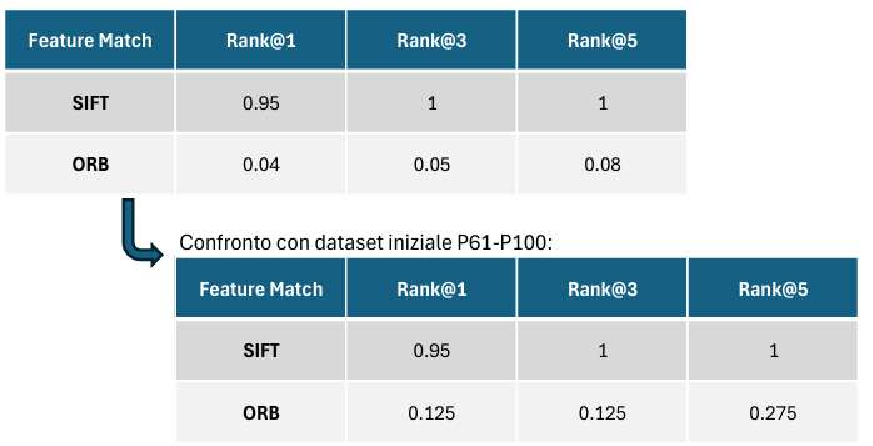
\includegraphics{figures/frontal1_1.pdf}
    	\caption{Accuracy Frontal Matching}
	\label{fig:frontal1}
\end{figure}
\begin{figure}[H]
	\centering
	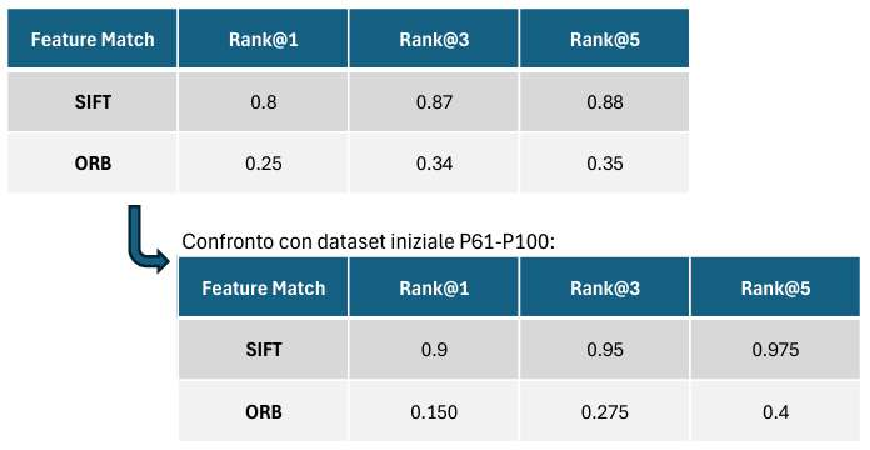
\includegraphics{figures/dx1_1.pdf}
   	\caption{Accuracy BTW DX Matching}
	\label{fig:dx1}
\end{figure}
\begin{figure}[H]
	\centering
	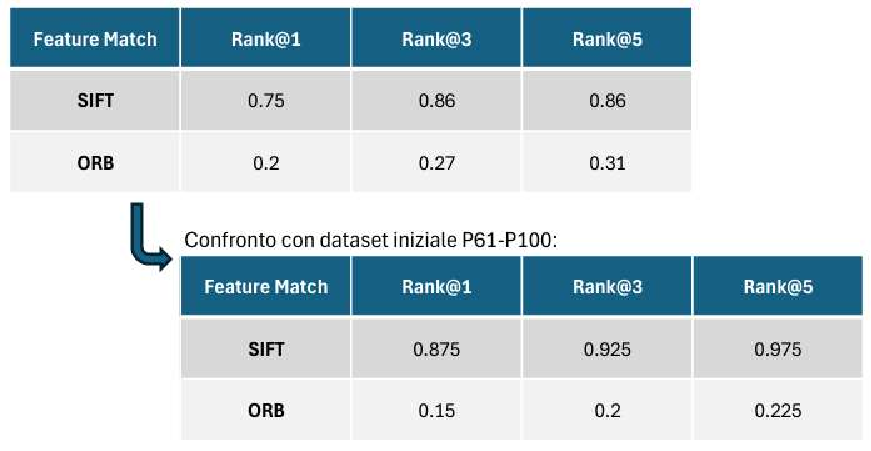
\includegraphics{figures/sx1_1.pdf}
   	\caption{Accuracy BTW SX Matching}
	\label{fig:sx1}
\end{figure}
\begin{figure}[H]
	\centering
	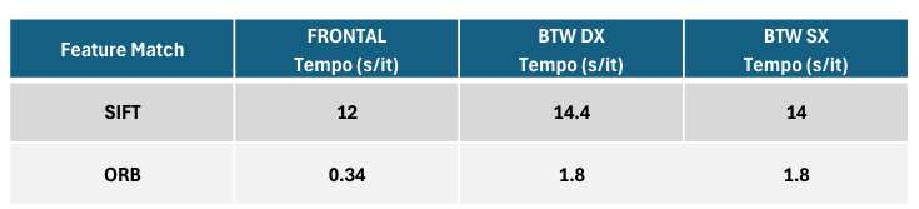
\includegraphics[height=3cm,width=13cm]{figures/tempi1.pdf}
    	\caption{Tempi di esecuzione con Dataset Aumentation}
	\label{fig:tempi1}
\end{figure}

L'impatto maggiore sui risultati, dobuto alla crescita della cardinalità del dataset, si manifesta sui tempi di esecuzione richiesti da algoritmi sofisticati, come SIFT. Il tempo necessario per eseguire tutti i match, per 100 query si aggira intorno ai 15 minuti; tempo non trascurabile a livello di prestazioni.\\
Il sistema, infatti, non è responsivo e richiede tempi di elaborazione troppo lunghi.\\

Le prestazioni ottenute, invece, sono diminuite,  a causa dell'aumento del numero di confronti richiesti.\\
Da questo punto, seguono diverse operazioni di modellamento al fine di realizzare un sistema che sia il più robusto, generale, preciso e veloce possibile.

%%%%%%%%%%%%%%%%%%%%%%%%%%%%%%%%%%%%%%%
\subsection{Il problema dei keypoint}
Il sistema che è stato realizzato implementa due algoritmi di Feature Matching per la ricerca di keypoint e calcolo dei relativi descrittori. \\
L'algoritmo così implementato, però, non è un algoritmo intelligente: infatti, effettua la ricerca sull'intera immagine di input.\\

Visivamente, un suo possibile risultato è il seguente:
\begin{figure}[H]
	\centering
	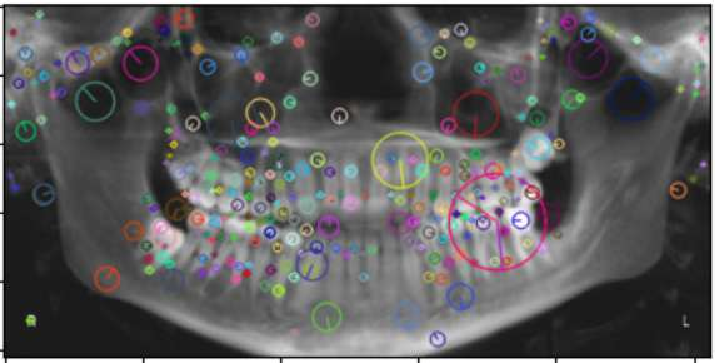
\includegraphics[width=14cm]{figures/keypointall.pdf}
    	\caption{Keypoint e Keypoint Descriptors}
	\label{fig:keypointall}
\end{figure}

Appare subito evidente come questa ricerca non sia finalizzata solo all'area di interesse. Tutti i keypoint e i relativi descrittori che non appartengono all'area dentale, non sono rilevanti, risultando addirittura fuorvianti nella ricerca del match ottimale.\\
E' necessario, perciò, raffinare la ricerca solo all'area di interesse, evitando errori di valutazione e il consumo di risorse inutilmente.


%%%%%%%%%%%%%%%%%%%%%%%%%%%%%%%%%%%%%%
\chapter{Algoritmi di Masking}
Appartenente alla famiglia delle tecniche di pre-processing di immagini, riveste particolare importanza la tecnica di \textbf{Masking}. \\
Il {\itshape masking}, in Computer Vision, è una tecnica largamente utilizzata allo scopo di selezionare o evidenziare particolari regioni di interesse all'interno di un'immagine, ignorandone, di conseguenza, le altre. Questa tecnica è utile in una vasta gamma di applicazioni, tra cui: {\itshape segmentazione delle immagini, rilevamento degli oggetti, elaborazione di immagini e Visione Artificiale}.\\
In particolare, è importante evidenziare alcune di queste applicazioni: 
\begin{enumerate}
\item \textbf{Segmentazione delle Immagini}:
Il masking è essenziale per operare una prima segmentazione delle immagini, quando l'obiettivo consiste nel separare specifiche regioni di interesse dell'immagine, determinate sulla base di alcune caratteristiche particolari come: colore, intensità o texture. \\
Si vogliono distinguere due tipologie principali di segmentazione:
\begin{itemize}
\item \textbf{Semantic Segmentation}: Ogni pixel dell'immagine viene classificato in una categoria specifica (es. cielo, strada, edifici).
\item \textbf{Instance Segmentation}: Simile alla precedente, ma differenzia anche tra diverse istanze della stessa classe (es. due persone separate).
\end{itemize}

\item \textbf{Rilevamento degli Oggetti}:
Il masking può essere utilizzato per creare {\itshape maschere binarie} al fine di evidenziare la presenza e la posizione di oggetti specifici di interesse in un'immagine. Le tecniche più avanzate includono l'utilizzo di {\itshape reti neurali}.

\item \textbf{Elaborazione delle Immagini}:
In vari processi di elaborazione delle immagini, il masking può essere usato per applicare trasformazioni solo a certe parti di un'immagine, come: filtraggio, correzione del colore o rimozione di oggetti.

\item \textbf{Inpainting e Super-Resolution}:
Il masking può essere utilizzato per compiti di inpainting (riempimento di parti mancanti di un'immagine) o super-resolution (miglioramento della risoluzione di un'immagine). In questi casi, una maschera indica le aree da ripristinare o migliorare.
\end{enumerate}

Tra le tecniche di masking più utilizzate ci sono:
\begin{itemize}
\item \textbf{Maschere Binarie}:
Una maschera binaria è un'immagine con due valori (0 e 1) che indica quali parti dell'immagine devono essere considerate (1) e quali devono essere ignorate (0).
\item \textbf{Maschere di Rete Neurali}:
Utilizzare una rete neurale per generare una maschera che segmenti l'immagine evidenziando diversi oggetti di interesse.
\end{itemize}

Sono tantissimi i campi in cui trova impiego questa tecnica, tra i più noti si possono citare:
\begin{itemize}
\item \textbf{Riconoscimento facciale}: Nascondere aree irrilevanti al fine di concentrare l'analisi unicamente sull'area del viso.
\item \textbf{Navigazione autonoma}: Identificazione di strade e di segnali stradali.
\item \textbf{Medicina}: Segmentazione di immagini mediche al fine di identificare tumori o altre patologie (viste come anomalie).
\item ecc.
\end{itemize}
Tantissimi sono i vantaggi offerti dalla tecnica di Masking, tra cui:
\begin{itemize}
\item \textbf{Precisione}: Consente di isolare aree specifiche per un'analisi più mirata.
\item \textbf{Efficienza}: Riduce il rumore e le informazioni irrilevanti, migliorando le prestazioni di modelli di Visione Artificiale.
\item \textbf{Versatilità}: Può essere applicata in vari campi, dalla sicurezza, alla medicina o alla robotica.
\end{itemize}
Il masking è, quindi, una tecnica fondamentale nei progetti di Computer Vision, essenziale per molte applicazioni avanzate al fine di migliorarne la precisione e l'efficienza nei sistemi di analisi delle immagini.\\

%%%%%%%%%%%%%%%%%%%%%%%%%%%%%%%%%%%%%%%%%%%%%%%%
\section{Masking for teeth identification}
Con lo scopo di realizzare un sistema robusto e generale, viene implementato un opportuno algoritmo di estrazione di {\itshape maschere binarie}.\\
L'algoritmo si basa sulla realizzazione di una rete neurale molto conosciuta per la Semantic Segmentation: \textbf{U-Net}.
\begin{figure}[H]
  	\centering
   	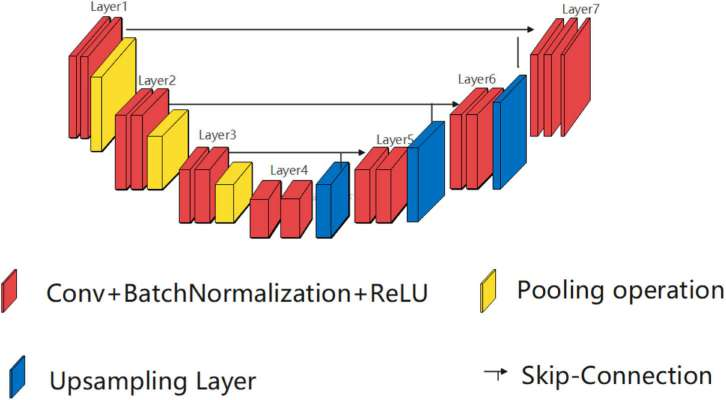
\includegraphics[width=14cm]{figures/unet.pdf}
    	\caption{Esempio di architettura di una rete CNN U-Net}
	\label{fig:unet}
\end{figure}

La CNN di seguito presentata, ha lo scopo di effettuare una {\itshape semantic segmentation} al fine di delimitare le aree in cui si individua la presenza di denti, rispetto a quelle contrarie. Nello specifico, viene presentata una particolare rete convoluzionale, denominata \textbf{GAN (Generative Adversarial Network)}.\\

L'architettura proposta presenta alcuni componenti chiave:
\begin{enumerate}
\item \textbf{Encoder-Decoder}: L'architettura encoder riduce la dimensione spaziale mantenendo le informazioni rilevanti, mentre il decoder si occupa di ricostruire l'immagine. Le skip connections aiutano a preservare dettagli rilevanti, durante il processo di risalita.
\item \textbf{Generatore}: Produce la maschera di output. Utilizza convoluzioni trasposte, al fine di ripristinare la dimensione spaziale di partenza.
\item \textbf{Discriminatore}: Distingue maschere generate da maschere reali, consentendo al generatore un'ottimizzazione.
\item \textbf{GAN}: Allena il generatore e il discriminatore insieme, secondo la modalità  "a somma zero".
\end{enumerate}

In generale, infatti, una Generative Adversarial Network (GAN) è un tipo di rete neurale utilizzata per generare nuovi dati a partire da un set di dati di addestramento. Una GAN è costituita da due componenti principali: il Generatore e il Discriminatore. Questi due modelli vengono addestrati insieme in modo antagonista.
\begin{itemize}
\item Generatore:
\begin{itemize}
\item {\itshape Scopo}: Generare nuovi dati simili ai dati di addestramento.
\item {\itshape Funzionamento}: Prende come input un vettore casuale (spesso chiamato rumore) e produce dati che cercano di imitare i dati reali.
\end{itemize}
\item Discriminatore:
\begin{itemize}
\item {\itshape Scopo}: Distinguere tra dati reali e dati generati.
\item {\itshape Funzionamento}: Prende come input un dato (che può essere reale o generato) e produce una probabilità che indica quanto sia reale il dato.
\end{itemize}
Il generatore viene addestrato per ingannare il discriminatore. L'obiettivo è minimizzare la capacità del discriminatore di distinguere tra dati reali e dati generati.\\
\end{itemize}
Al fine di ottemperare a queste funzionalità, sono state definite opportuni moduli che ne definiscono la struttura:
\begin{enumerate}
\item \textbf{convolution}:\\
Esegue una convoluzione 2D, seguita da una normalizzazione a gruppi (Group Normalization) e un'attivazione non lineare.\\
Nel caso in cui la convoluzione faccia parte del decoder ({\itshape conv\_type == 'decoder'}), vengono aggiunte ulteriori convoluzioni e normalizzazioni con l'aumento dei filtri, seguite dall'attivazione.\\
Infine, utilizza una connessione di shortcut tramite {\itshape layers.average} che fonde il risultato della convoluzione con una convoluzione a 1x1 del dato d'ingresso.

\item \textbf{encoder}:\\
Esegue delle convoluzioni e una normalizzazione; effettua un downsampling, con {\itshape AveragePooling2D}, al fine di ridurre la dimensionalità dell'immagine.\\
Restituisce sia il risultato convoluto (che verrà ulteriormente elaborato), sia una skip connection, usata successivamente nel decoder.

\item \textbf{decoder}:\\
Esegue una convoluzione trasposta per risalire nella dimensione spaziale (equivalente a un'operazione di upsampling).\\
Combina il risultato con la rispettiva skip connection dall'encoder (fusione tramite {\itshape layers.average}), al fine di preservare dettagli a diverse scale di risoluzione.\\
Continua con ulteriori convoluzioni e normalizzazioni, similmente a quanto accade nella funzione convolution.

\item \textbf{generator}:\\
Implementa una rete encoder-decoder profonda. Ogni livello dell'encoder riduce la dimensione spaziale e aumenta il numero di filtri, mentre il decoder ripristina la risoluzione spaziale.\\
Utilizza attivazioni \textbf{LeakyReLU} nell'encoder e \textbf{ReLU} nel decoder.\\
Al termine, genera l'output (la maschera) tramite una convoluzione trasposta con attivazione sigmoide.

\item \textbf{discriminator}:\\
Prende come input un'immagine e una maschera e li moltiplica (operazione {\itshape multiply}), combinandoli al fine di discriminare una maschera reale da una generata.\\
Successivamente, passa l'input combinato attraverso un'architettura encoder simile a quella del generatore.\\
Al termine, un {\itshape GlobalAveragePooling2D}, seguito da un{\itshape Dense layer}, produce un output scalare che rappresenta la stima del discriminatore del corretto funzionamento.\\
Viene poi eseguito insieme ad una {\itshape loss function} e ad un ottimizzatore, al fine di effettuare l'addestramento.

\item \textbf{GAN}:\\
Combina il generatore e il discriminatore in un modello GAN.\\
Il discriminatore è congelato durante l'addestramento del GAN, allo scopo di addestrare unicamente il generatore.\\
L'output del GAN è la probabilità che il discriminatore classifichi correttamente l'immagine generata.
\begin{figure}[H]
  	\centering
    	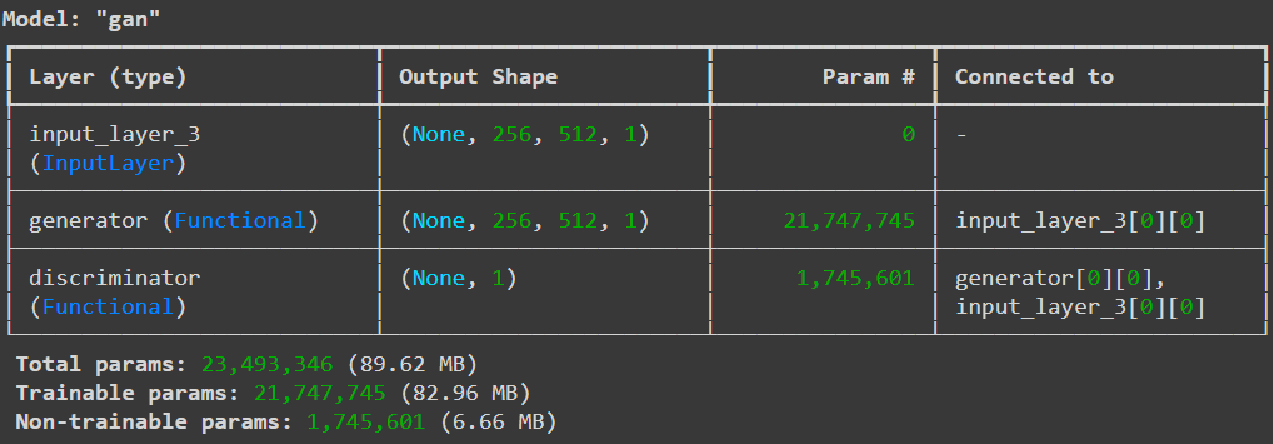
\includegraphics[width=16cm]{figures/gan.pdf}
   	\caption{Modello GAN}
	\label{fig:gan}
\end{figure}

\item \textbf{Addestramento GAN}:\\
Il ciclo di addestramento iterativo allena:
\begin{itemize}
\item Il discriminatore, a distinguere tra maschere reali e maschere generate.
\item Il generatore ad ingannare il discriminatore.
\end{itemize}

\item \textbf{Addestramento del generatore}:\\
Per ultimo, il generatore viene addestrato separatamente (dopo che alcune sue parti sono state congelate), attraverso l'ausilio di una loss specifica (come {\itshape BinaryFocalCrossentropy}) e metriche di precision e recall al fine di valutare le prestazioni.
\end{enumerate}

%%%%%%%%%%%%%%%%%%%%%%%%%%%%%%%%%%%%
\subsection{Leaky ReLU e ReLU}
In Computer Vision e, più in generale, nelle reti neurali, la funzione \textbf{ReLU} (Rectified Linear Unit) e la funzione \textbf{Leaky ReLU} sono entrambe {\itshape funzioni di attivazione}, utilizzate al fine di introdurre non linearità nel modello. Queste funzioni aiutano la rete a imparare rappresentazioni complesse dai dati, come immagini, segnali o sequenze. In particolare:
\begin{enumerate}
\item \textbf{ReLU}:\\
La funzione ReLU è una delle funzioni di attivazione più utilizzate nelle reti neurali profonde. È definita semplicemente dalla seguente formula:

\begin{figure}[H]
  	\centering
   	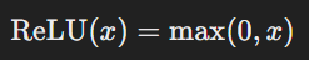
\includegraphics[height=1cm, width=5cm]{figures/relu.pdf}
    	\caption{Funzione di attivazione ReLU}
	\label{fig:relu}
\end{figure}

\begin{itemize}
\item Se il valore di input è positivo, ReLU restituisce lo stesso valore.
\item Se il valore di input è negativo, ReLU restituisce 0.
\end{itemize}

I vantaggi nel suo utilizzo sono:
\begin{itemize}
\item {\itshape Computazione semplice}: Richiede solo un confronto tra 0 e l'input, risultando computazionalmente efficiente.
\item {\itshape Sparsità}: Molti neuroni possono avere output 0, il che aiuta a ridurre il carico computazionale e rende il modello più efficiente.
\item{\itshape Evita saturazione positiva}: A differenza di altre funzioni di attivazione come {\itshape sigmoid} o {\itshape tanh}, ReLU non soffre di saturazione nella parte positiva, permettendo un apprendimento più rapido.
\end{itemize}
Viceversa, esistono anche alcuni svantaggi indotti dall'utilizzo di questa particolare funzione, come:
\begin{itemize}
\item {\itshape Morte dei neuroni ReLU}: Se durante l'allenamento molti neuroni ottengono input negativi, il loro output diventa sempre zero, il che può portare a neuroni "morti", ossia, non vengono più aggiornati durante la backpropagation.
\end{itemize}

\item \textbf{Leaky ReLU}:
Al fine di risolvere il problema dei neuroni morti in ReLU, è stata introdotta la funzione Leaky ReLU.  Diversamente da ReLU, invece di forzare un output a 0 per gli input negativi, Leaky ReLU restituisce un piccolo valore negativo (in genere una frazione dell'input, come 0.01 * x).\\
Più specificatamente, la funzione è definita come:

\begin{figure}[H]
  	\centering
    	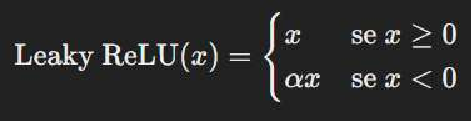
\includegraphics[height=2cm, width= 7cm]{figures/leaky.pdf}
    	\caption{Funzione di attivazione Leaky ReLU}
	\label{fig:leaky}
\end{figure} 
Dove $\alpha$ è un piccolo valore positivo, tipicamente $\alpha$ = 0.01.

I vantaggi offerti da questo modello sono:
\begin{itemize}
\item {\itshape Assenza di neuroni morti}: Gli input negativi non vengono forzati a zero, ma moltiplicati per un piccolo valore; tutti i neuroni possono, perciò, contribuire al gradiente e continuare l'apprendimento.
\item {\itshape Performance migliori in alcuni casi}: Può migliorare la performance rispetto a ReLU quando devono essere gestiti molti input negativi.
\end{itemize}

Uno svantaggio introdotto, però, è il seguente:
\begin{itemize}
\item Il valore di $\alpha$ è un iperparametro e, come tale, deve essere scelto a priori; perciò, potrebbe richiedere diverse fasi di tuning al fine di migliorare i risultati ottenuti.
\end{itemize}

In generale è possibile dire che:
\begin{itemize}
\item ReLU è più semplice ed efficiente nella maggior parte dei casi, ma potrebbe causare il  problema dei neuroni morti.
\item Leaky ReLU è una versione modificata che riduce il rischio dei neuroni morti, ma può richiedere più attenzione nella fase di tuning.
\end{itemize}
\end{enumerate}

%%%%%%%%%%%%%%%%%%%%%%%%%%%%%%%%%%%%%%%%%%5
\subsection{L'algoritmo}
L'algoritmo così implementato, viene addestrato su un dataset di 598 immagini ortopanoramiche; per ognuna, viene presa in input la rispettiva maschera delineata manualmente. Viene effettuato uno split del dataset, in train e validation set, il secondo composto da 80 immagini; viene effettuato similmente lo split dalle rispetttive maschere.\\
La rete neurale viene addestrata, aggiornando i corrispondenti pesi.\\
Il processo viene ripetuto ricorsivamente sui nuovi pesi, per 10000 epoche. \\
Successivamente, viene ripetuto l'addestramento sulle immagini appartenenti al validation set per 160 epoche di addestramento. Al fine di evitare il rischio di overfitting, viene impostato un valore di {\itshape patience = 5}.\\

Il secondo addestramento è fondamentale ai fini della valutazione del modello di generazione delle maschere.\\
I risultati ottenuti sono molto buoni, con:
\begin{itemize}
\item \textbf{Accuracy}: 0.97
\item \textbf{Loss}: 0.02
\item \textbf{Precision}: 0.9
\end{itemize}

Graficamente, è possibile visualizzare come il modello si adatti perfettamente ai dati.
\begin{figure}[H]
    	\centering
    	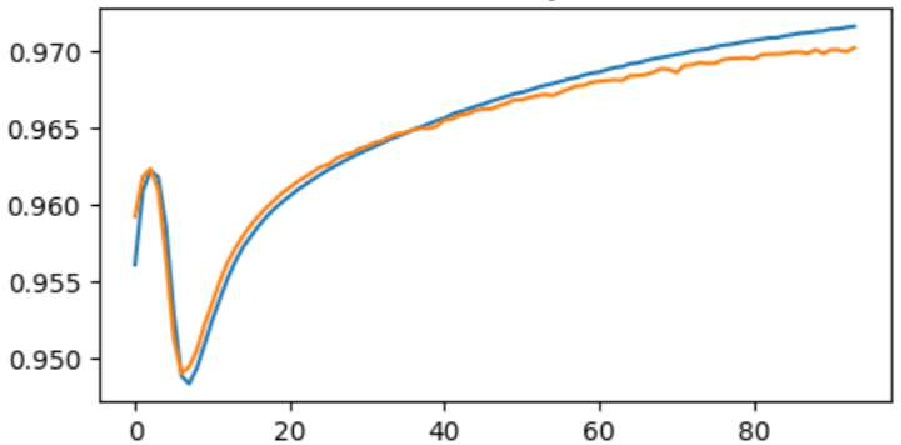
\includegraphics[height=5cm,width=9cm]{figures/accuracy.pdf}
    	\caption{Accuracy}
	\label{fig:accuracy}
\end{figure}
\begin{figure}[H]
    	\centering
    	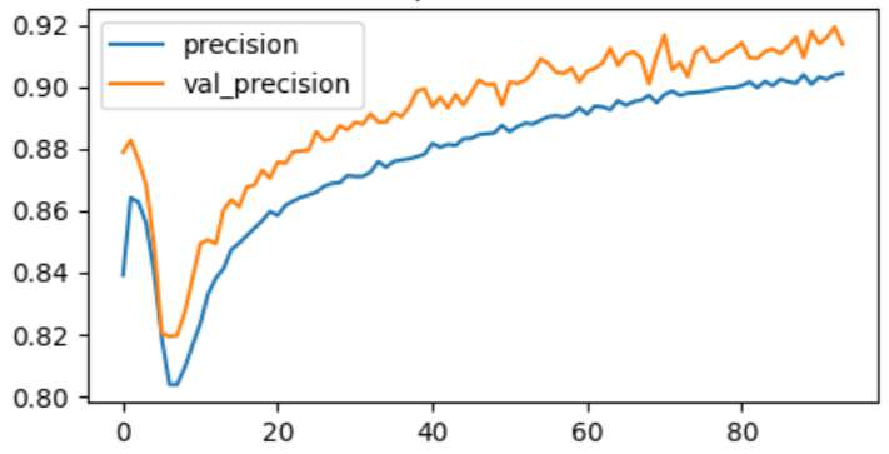
\includegraphics[height=5cm,width=9cm]{figures/precision.pdf}
    	\caption{Precision}
	\label{fig:precision}
\end{figure}
\begin{figure}[H]
    	\centering
   	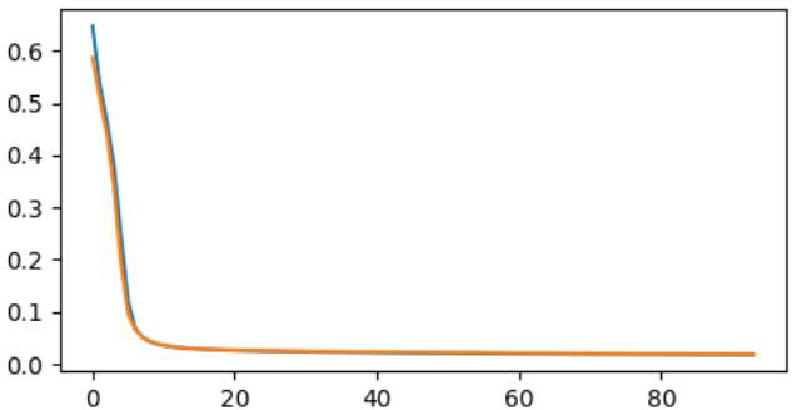
\includegraphics[height=5cm,width=9cm]{figures/loss.pdf}
    	\caption{Loss}
	\label{fig:loss}
\end{figure}

La terza fase, quella di testing, viene effettuata sulle immagini appartenenti al dataset delle ortopanoramiche precedentemente definito. Il risultato prodotto da questa fase, consiste in un dataset della stessa cardinalità di quello fornito in input, ma costituito dalle sole maschere binarie prodotte, ossia da immagini, in cui le parti evidenziate in bianco risiedono in corrispondenza delle aree dentali.
\begin{figure}[H]
    	\centering
    	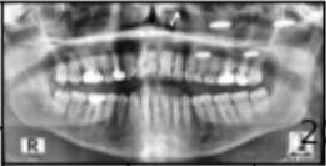
\includegraphics[height=4cm,width=8.5cm]{figures/mask_img.pdf}
   	\caption{Immagine di partenza}
	\label{fig:masking}
\end{figure}
\begin{figure}[H]
    	\centering
    	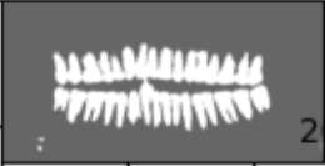
\includegraphics[height=4cm,width=8.5cm]{figures/mask_mask.pdf}
    	\caption{Maschera binaria estratta}
	\label{fig:mask}
\end{figure}
\begin{figure}[H]
    	\centering
   	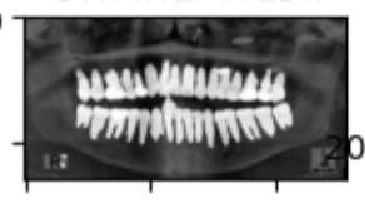
\includegraphics[height=4cm,width=8.5cm]{figures/mask_tot.pdf}
    	\caption{Sovrapposizione delle due immagini}
	\label{fig:masktot}
\end{figure} 

Una possibile evoluzione successiva, vedrebbe la realizzazione di maschere applicate al singolo dente. Questo tipo di applicazione è nota come {\itshape Instance Segmentation}. Essa consentirebbe, infatti, l'identificazione tramite maschere dei singoli denti.\\
A questo livello di sviluppo del progetto, però, è un livello di raffinamento non necessario, siccome, ai fini dell'identificazione dell'area in cui sono presenti i denti è sufficiente utilizzare un algoritmo di Semantic Segmentation.

%%%%%%%%%%%%%%%%%%%%%%%%%%%%%%%%%%%%%%%%%%%%%
\section{Estrazione dei keypoint con Maschere}
A queso punto è possibile combinare i risultati precedenti.\\
Gli algoritmi di Computer Vision per l'estrazione dei keypoint tramite {\itshape maschere binarie}, sono comunemente utilizzati al fine di identificare caratteristiche distintive all'interno di una determinata area dell'immagine. Le maschere binarie consentono di delimitare le aree su cui concentrarsi, filtrando le regioni di interesse (ROI) e ignorando quelle non rilevanti. Gli algoritmi di definizione dei keypoint vengono applicati, così, solo ai pixel all'interno della regione selezionata dalla maschera.\\
Questo raffinamento comporta una serie di vantaggi, tra cui:
\begin{itemize}
\item \textbf{Ricerca mirata}: Le maschere binarie permettono di evitare il calcolo sui pixel non rilevanti, migliorando l’efficienza complessiva dell'algoritmo di ricerca.
\item \textbf{Efficienza computazionale}: Riduce il numero di pixel su cui l'algoritmo deve lavorare, migliorandone la velocità.
\item \textbf{Riduzione del rumore}: Limita l’analisi solo alle aree di interesse, ignorando i dati di fondo non rilevanti.
\item \textbf{Controllo maggiore}: Consente un controllo più preciso sull'area di ricerca dei keypoint, utile per applicazioni specifiche come la segmentazione di immagini mediche o l'analisi di volti.
\end{itemize}

Vengono perciò combinati gli algoritmi di Feature Matching visti in precedenza, alle maschere binarie estratte attraverso la rete neurale.\\

Gli step di computazione possono essere sequenzializzati come segue:
\begin{enumerate}
\item \textbf{Estrazione delle feature}:
\begin{itemize}
\item def {\itshape extract\_features}
\item Input: Una lista di percorsi di immagini, un oggetto sift, e una lista facoltativa di percorsi per le maschere.
\begin{itemize}
\item Inizialmente, viene utilizzata per estrarre le feature dalle immagini ortopanoramiche attraverso l'ausilio delle maschere. Le maschere permettono, quindi, di restringere l'area di interesse di ricerca {\itshape solo} all'interno della zona evidenziata dalla maschera; le aree di colore bianco all'interno della maschera binaria, sono le zone la cui sovrapposizione con l'immagine corrispondente identifica l'area di ricerca.
\item In secondo luogo, viene utilizzata per la ricerca delle feature sull'immagine di query; viene posta la maschera a {\itshape None} e non viene definito nessun raffinamento più specifico.
\end{itemize}
\item Per ogni immagine, viene chiamata la funzione {\itshape image\_detect\_and\_compute}, a cui viene passata l'eventuale maschera.
\begin{itemize}
\item \textbf{image\_detect\_and\_compute}:
\begin{itemize}
\item Input: Un oggetto sift (SIFT detector), il percorso dell'immagine, il percorso facoltativo per una maschera binaria.
\item Viene letta l'immagine in scala di grigi.
\item Se viene fornita una maschera, essa viene caricata e verificato che abbia la stessa dimensione dell'immagine, altrimenti viene sollevato un errore.
\item Utilizza l'oggetto SIFT per rilevare i keypoint e calcolare i descrittori nell'area dell'immagine coperta dalla maschera (se presente).
\item In output: Ritorna l'immagine, i keypoint e i descrittori.
\begin{figure}[H]
	\centering
    	\lstinputlisting[language=Python,label={lst:kpwithmask}]{listings/detectcomputemask.py}
\end{figure} 
\end{itemize}
\end{itemize}
\item Vengono memorizzate  le informazioni relative a ciascuna immagine  in una lista di tuple (inclusi i keypoint e i descrittori).
\item In output, viene restituita una lista di tuple contenenti le informazioni di: {\itshape percorso dell'immagine, immagine stessa, keypoint, e descrittori}.
\end{itemize}

\item \textbf{Feature Matching}:
\begin{itemize}
\item def {\itshape match\_images}.
\item Input: Due set di descrittori (des1 e des2), un metodo di matching (FLANN o brute force), e un parametro k per il numero di vicini più prossimi da considerare.
\item La funzione verifica se i descrittori sono validi ed esegue il matching tra i descrittori utilizzando il metodo specificato:
\begin{itemize}
\item FLANN: Usa una struttura K-D tree per il matching rapido.
\item Brute force (BFMatcher): Confronta direttamente le coppie di descrittori.
\end{itemize}
\item Viene eseguito il \textbf{ratio test di Lowe}, al fine di migliorare la qualità del matching, mantenendo solo i match con una distanza relativa bassa tra i due descrittori.
\item In output: Viene restituita una lista di match validi.
\end{itemize}

\item \textbf{Ricerca dei migliori match}:
\begin{itemize}
\item Per ogni immagine di query, viene eseguito il matching delle feature usando {\itshape match\_images}.
\item Vengono ordinate le immagini ortopanoramiche confrontate, sulla base del numero di match individuati, in ordine decrescente.
\item In output: Vengono restituiti i primi {\itshape top\_n match}, insieme alle informazioni di: nome dell' immagine ortopanoramica e relativo numero di match.
\end{itemize}

\item \textbf{Valutazione dell'accuratezza del matching}:
\begin{itemize}
\item Per ogni immagine di query, viene controlato se all'interno della lista dei migliori match individuati è presente quello relativo all'immagine ortopanoramica corretta.
\item In caso positivo, viene incrementato il contatore relativo alla posizione individuata, rispettivamente se presente nella posizione 1, o entro le prime 3 o 5 posizioni.
\item Viene calcolata, infine, l'\textbf{accuratezza} delle predizioni rispetto ai Rank@1, Rank@3, e Rank@5 (precisione nell'individuare il match corretto nei primi 1, 3 o 5 match migliori).
\item In output: Vengono restituiti i valori di accuracy individuati.
\end{itemize}
\end{enumerate}

%%%%%%%%%%%%%%%%%%%%%%%%%%
\subsection{Scelta di k e Lowe's Ratio Test}
La scelta di k deve essere effettuata in maniera corretta, al fine di ottenere un confronto significativo tra più vicini. Solitamente, k viene impostato a 2 per permettere l'uso del Lowe's ratio test.\\
Il \textbf{Lowe's ratio test} confronta il miglior match con il secondo miglior match, al fine di filtrare i falsi positivi. Perché questo test funzioni, è necessario avere almeno 2 vicini per ogni descrittore. Se la distanza del miglior match non è significativamente più bassa (di $solito < $0.85) rispetto al secondo, il match viene considerato un falso positivo. Questo è particolarmente utile in scenari in cui ci sono molte caratteristiche simili e il rischio di ottenere match errati è alto.

%%%%%%%%%%%%%%%%%%%%%%%%%%%%
\subsection{Feature Extraction con Masking}
E' possibile visualizzare i benefici introdotti dall'ausilio di opportune maschere nella ricerca dei keypoint, e calcolo dei relativi descrittori, in un'immagine ortopanoramica.

\begin{figure}[H]
  	\centering
    	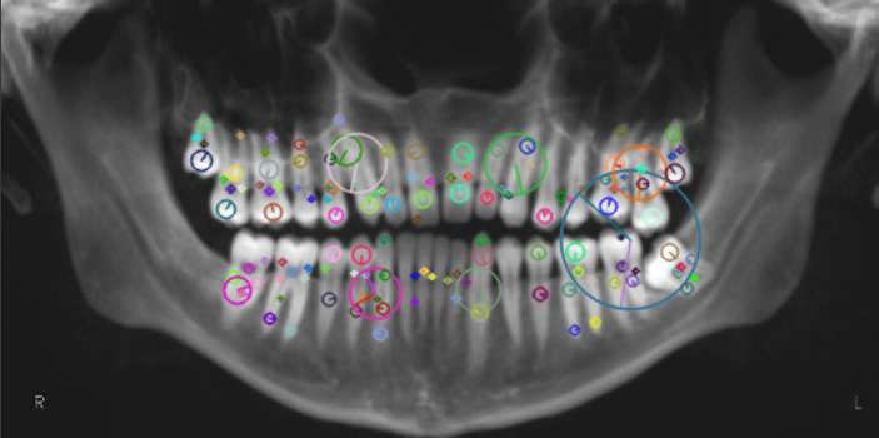
\includegraphics{figures/kpmask.pdf}
    	\caption{Feature Extraction con Masking}
	\label{fig:kpmask}
\end{figure} 

Risulta subito evidente come, attraverso l'ausilio delle maschere, sia possibile concentrare la ricerca dei punti di interesse {\itshape solo} nell'area coperta dalla relativa maschera, ossia quella identificativa dell'area dentale.


%%%%%%%%%%%%%%%%%%%%%%%%%%55
\subsection{Problemi introdotti}
Attraverso l'ausilio delle maschere viene a manifestarsi un nuovo problema, durante il processo di Feature Matching.\\
L'algoritmo, per come è stato definito, effettua un processo di ricerca dei migliori match utilizzando una misura di distanza: {\itshape knnMatch}.\\

La funzione \textbf{knnMatch()}, di OpenCV, è ampiamente utilizzata al fine di effettuare il matching dei descrittori; essa si basa sul concetto di k-nearest neighbors (k-NN). Tuttavia, ci sono alcuni vincoli e considerazioni importanti che devono essere valutati prima del suo utilizzo, tra cui:
\begin{itemize}
\item \textbf{Numero minimo di descrittori}:\\
Entrambi i set di descrittori devono avere {\itshape almeno} k descrittori, dove k è il numero di vicini più prossimi da ricercare, per ogni descrittore.\\
Se uno dei set di descrittori ha meno di k elementi, non è possibile trovare k vicini per ogni descrittore; la funzione solleva un errore o restituisce risultati non validi. \\
Nell'algoritmo implementato \textbf{k=2}; il set di descrittori deve contenere almeno 2 descrittori.

\item \textbf{Tipo di dati dei descrittori}:\\
I descrittori devono essere in formato \textbf{float32}, se si utiizza il matcher FLANN.\\
L'algoritmo FLANN (Fast Library for Approximate Nearest Neighbors), spesso usato in combinazione con knnMatch, richiede che i descrittori siano di tipo float32 per eseguire il matching. Se i descrittori sono in un formato diverso (ad esempio int), la funzione non funziona correttamente.

\item \textbf{Comparabilità dei descrittori}:\\
I descrittori devono essere estratti dallo stesso tipo di feature (ad esempio, SIFT con SIFT, oppure ORB con ORB). \\
Se si utilizzano descrittori generati con algoritmi differenti (ad esempio, SIFT contro ORB), knnMatch() non funziona correttamente, perché i descrittori avranno dimensioni e valori differenti. I descrittori devono essere comparabili, ossia, provenire dallo stesso metodo di estrazione delle feature.

\end{itemize}

Attraverso l'ausilio delle maschere viene ridotto notevolemente il rumore e scompare, quasi totalmente, il problema relativo all'estrazione di keypoint in punti non appartenenti alla RoI.\\

Eseguendo l'algoritmo senza opportuni controlli, vengono riportati una serie di messaggi di errore relativi alla mancata, o insufficiente, estrazione di keypoint o relativi alla bassa dimensionalità dei descrittori.\\

Questi errori, nella versione iniziale dell'algoritmo, non venivano riscontrati. Ora, invece, sono provocati da due fattori:
\begin{enumerate}
\item Accrescimento della cardinalità e variabilità del dataset di ortopanoramiche.
\item Estrazione dei keypoint {\itshape unicamente} all'interno della RoI.
\end{enumerate}

Analizzando i casi in cui gli errori vengono riscontrati, è possibile visualizzarne la causa:
\begin{figure}[H]
  	\centering
	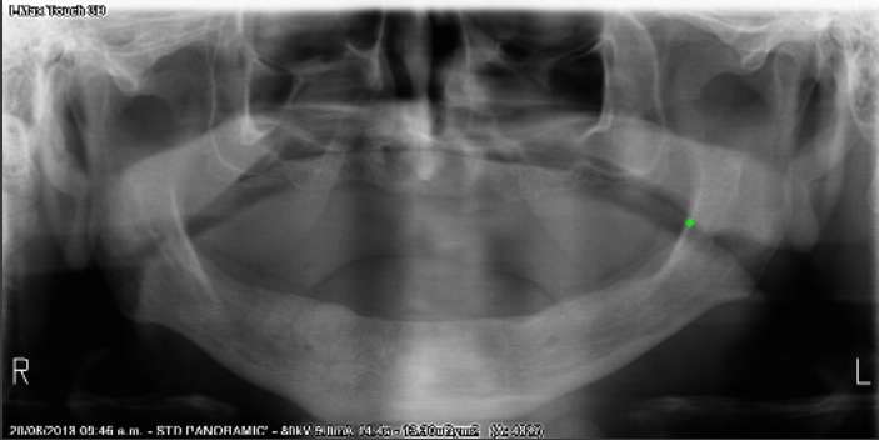
\includegraphics{figures/nodenti.pdf}
   	\caption{Assenza di denti}
	\label{fig:nodenti}
\end{figure} 

In casi di assenza totale o bassa cardinalità del numero di denti presenti in un'immagine ortopanoramica, il numero dii keypoint e la dimensione dei relativi descrittori è bassa, se non addirittura nulla. E' necessario, perciò, introdurre opportuni controlli prima di effettuare la valutazione del Matching.
\begin{enumerate}
\item \textbf{Numero minimo di descrittori}: Prima di chiamare knnMatch, è necessario verificare che il numero di descrittori sia maggiore o uguale a k (con k=2) su entrambi i set di descrittori.
\item \textbf{Tipo di dati dei descrittori}: I descrittori vengono convertiti in float32, prima di calcolare knnMatch.
\end{enumerate}
Di conseguenza, nel caso in cui dovessero essere individuati dei descrittori che non rispettano tali vincoli, il matching viene saltato.

\begin{figure}[H]
	\centering
    	\lstinputlisting[language=Python,label={lst:kpcontrol}]{listings/controllokp.py}
\end{figure} 

%%%%%%%%%%%%%%%%%%%%%%%%%%%%%%%%%%%%%%%%%5
\subsection{Risultati ottenuti}
Vengono confrontati i risultati ottenuti, con questo tipo di computazione, rispetto ai risultati ottenuti nei punti precedenti.
\begin{figure}[H]
	\centering
	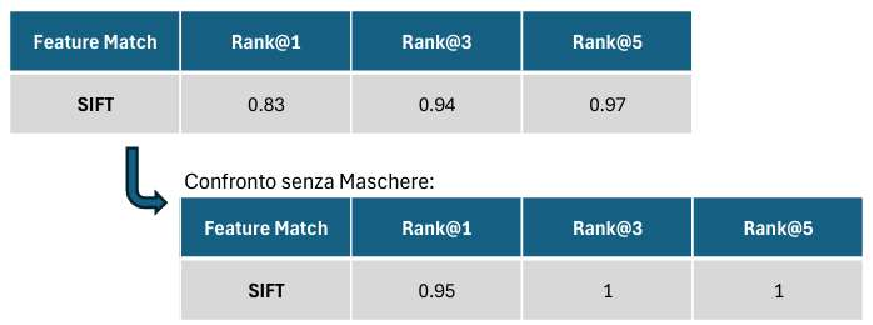
\includegraphics{figures/frontal2_1.pdf}
    	\caption{Accuracy Frontal Matching con Masking}
	\label{fig:frontal2}
\end{figure}
\begin{figure}[H]
	\centering
	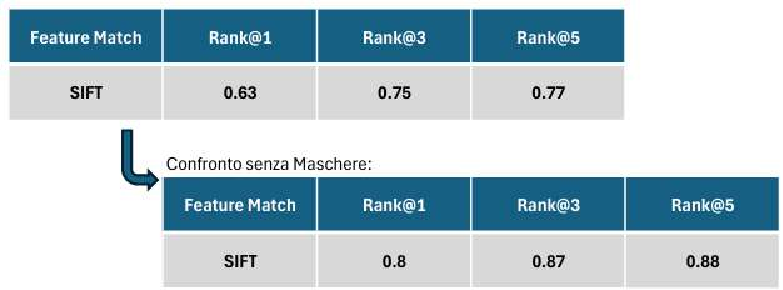
\includegraphics{figures/dx2_1.pdf}
    	\caption{Accuracy BTW DX Matching con Masking}
	\label{fig:dx2}
\end{figure}
\begin{figure}[H]
	\centering
	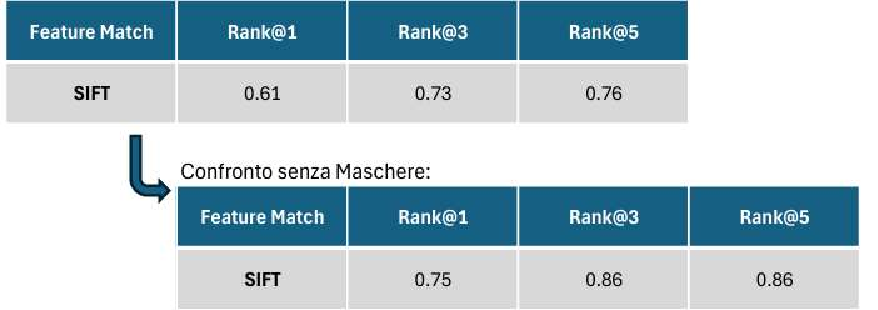
\includegraphics{figures/sx2_1.pdf}
    	\caption{Accuracy BTW SX Matching con Masking}
	\label{fig:sx2}
\end{figure}
\begin{figure}[H]
	\centering
	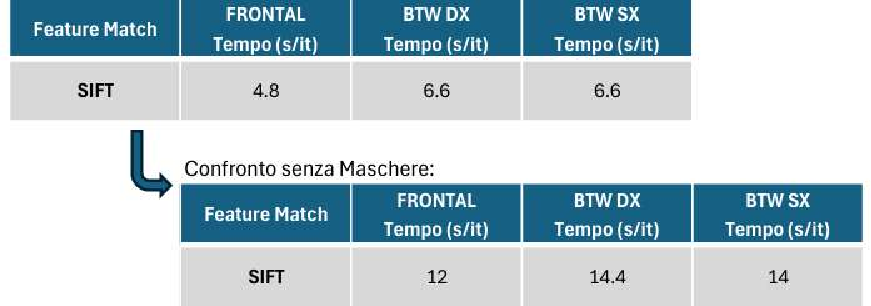
\includegraphics{figures/tempi2_1.pdf}
   	\caption{Tempi di esecuzione con Masking}
	\label{fig:tempi2}
\end{figure}
Un esempio di Feature Matching che sfrutta l'ausilio delle maschere, è il seguente:
\begin{figure}[H]
	\centering
	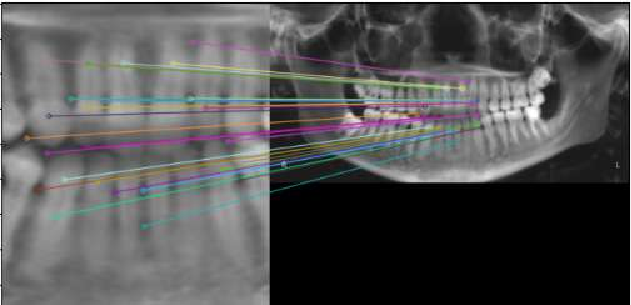
\includegraphics[width=15cm,height=7cm]{figures/matchmask.pdf}
    	\caption{Feature Matching con Masking}
	\label{fig:matchmask}
\end{figure}

L'area di matching, attraverso l'ausilio delle maschere, è priva di outlier (punti al di fuori dell'area dentale).\\

Dalle tabelle dei valori di accuracy ottenuti è possibile constatare che:
\begin{itemize}
\item I valori di accuracy sono, in generale, diminiuiti.
\item I tempi richiesti per il singolo match, sono dimininuiti.
\end{itemize}

Il sistema così progettato, è diventato più efficiente e consistente. I tempi richiesti per il processamento sono notevolmente diminuiti, questo a fronte del fatto che:
\begin{itemize}
\item I keypoint individuati sono ristretti alla sola area di interesse; diminuisce, dunque, il numero complessivo di punti non significativi individuati.
\item Diminuisce il numero dei corrispondenti descrittori e, di conseguenza, diminuisce il numero di confronti da dover effettuare.
\end{itemize}
Viene, perciò, migliorata l'efficienza del sistema di match e la reattività del sistema di risposta.\\

Per quanto riguarda i valori di accuracy, questi sono diminuiti; il livello di precisione, invece, è aumentato, a fronte del fatto che viene ristretto il campo di ricerca.\\
Come conseguenza inevitabile e naturale, dovuta alla ricerca dei keypoint che, ora, è incentrata unicamente nell'area di interesse, il valore di accuracy diminuisce ma diminuisce anche il valore dei falsi positivi. Nei casi precedenti, infatti, molti match individuati, non erano corretti.\\
A causa della struttura dell'immagine in esame, i keypoint hanno caratteristiche molto simili tra di loro e risulta perciò difficile la reciproca distinzione. Per quantità maggiori di keypoint individuati, aumenta corrispondentemente anche il numero di match errati. \\
In seguito alla restrizione dell'area di ricerca, a discapito dei valori di accuracy, i match restituiti sono, in percentuale, molto più corretti. \\
Complessivamente, dunque, i risultati restituiti sono molto buoni e il sistema ottenuto risulta più robusto, efficiente, reattivo e corretto.

%%%%%%%%%%%%%%%%%%%%%%%%%%%%%%%%%%%%%%%%%%%%%%%
\subsection{Il problema della RoI}
Attraverso l'utilizzo delle maschere, il processo di feature matching risulta più accurato e robusto.\\
A questo punto, però, è possibile eseguire un ulteriore passo di raffinamento.\\

I match che vengono effettuati, richiedono il confronto tra un'immagine di query e il dataset delle immagini ortopanoramiche. Le immagini di query possono essere:
\begin{itemize}
\item Radiografie frontali.
\item Radiografie laterali, destra e sinistra.
\end{itemize}

Di conseguenza, effettuare il match di un'immagine di bitewing, frontale o laterale, nell'intera sezione dell'area dentale, può essere fuorviante e a complessità maggiore e non necessaria.\\
Infatti, il matching tra un'immagine di query frontale rispetto ad un'immagine ortopanoramica, non necessita il confronto tra descrittori dell'ortopanoramica, esterni alla zona centrale dell'area dentale.\\
A seguito di questa considerazione, è possibile definire una Region of Interest più restrittiva, che mira più specificatamente alla zona di interesse. 


%%%%%%%%%%%%%%%%%%%%%%%%%%%%%%%%%%%%%%%%%%%%%%
\chapter{Restringimento delle RoI}
Come precedentemente introdotto, è possibile effettuare un ulteriore restringimento della RoI, delimitando l'area di ricerca nel processo di matching, alla sola zona di interesse dell'immagine di querying.\\
A tale scopo, dunque, vengono individuate le aree di interesse attraverso un processo di estrazione delle RoI sulle maschere.\\
L'idea, infatti, è quella utilizzare i benefici introdotti dall'utilizzo delle maschere binarie applicate alle immagini ortopanoramiche. La maschera, ora, viene ristretta alla sola area di interrogazione: frontale per le immagini "FRONTAL\_n" e laterale destra e sinistra per le immagini "BTW DX\_n" e "BTW SX\_n".\\

Vengono definite apposite funzioni di elaborazione di immagine:
\begin{enumerate}
\item \textbf{detect\_white\_region}:
\begin{itemize}
\item Ha lo scopo di rilevare la bounding box più esterna che racchiude tutte le regioni bianche presenti all'interno della maschera binaria.
\item A tale scopo, viene applicata una soglia binaria all'immagine, al fine di ottenere una maschera con pixel bianchi (valore 255) e neri (valore 0). Viene utilizzata la soglia 254 per catturare solo le aree bianche con valore 255.
\item Viene utilizzata la funzione {\itshape cv2.findContours()} per rilevare i contorni delle regioni bianche.
\item Se non vengono individuati contorni, viene restituito {\itshape None}.
\item Viceversa, per ogni contorno individuato, calcola la bounding box utilizzando la funzione {\itshape cv2.boundingRect()}, e aggiornando i valori minimi e massimi delle coordinate x e y al fine di ottenere la bounding box totale che racchiude tutte le regioni bianche.
\item In output, vengono restituite le coordinate della bounding box: \{x\_min, y\_min, x\_max, y\_max\}.
\end{itemize}

\item \textbf{get\_central\_part\_of\_bbox}:
\begin{itemize}
\item Ha lo scopo di estrarre la parte centrale della bounding box rilevata dall'immagine originale, basandosi su un parametro di rapporto centrale ({\itshape central\_ratio}), che specifica quale proporzione della larghezza della bounding box mantenere.
\item Data in input l'immagine,  viene calcolata la larghezza della RoI sulla base della bounding box individuata, attraverso l'utilizzo della funzione precedente, e del valore di central\_ratio. Viene poi ristretta sulla base del valore specificato. 
\item Viene calcolato il centro della bounding box. Viene mantenuta inalterata l'altezza.
\item Viene così inizializzata una nuova maschera, della stessa dimensione dell'immagine di partenza.
\item Viene poi copiata solo la parte centrale, individuata precedentemente, dalla maschera originale.
\item In output, viene restituita la nuova maschera, che individuerà una nuova area di ricerca più restrittiva.
\end{itemize}

\begin{figure}[H]
	\centering
    	\lstinputlisting[language=Python,label={lst:roi}]{listings/roi.py}
\end{figure} 

\item \textbf{get\_dx\_part\_of\_bbox}:
\begin{itemize}
\item Ha lo scopo di estrarre la parte destra della bounding box, dall'immagine di masking originale.
\item Data la larghezza della bounding box e il valore di {\itshape lateral\_ratio}, viene determinata la larghezza della regione destra che si vuole mantenere.
\item Vengono, perciò, calcolate le nuove coordinate della bounding box destra. Le coordinate verticali rimangono, invece, inalterate.
\item Similmente a quanto visto prima, viene inizializzata una maschera vuota della stessa dimensione dell'immagine.
\item Viene poi copiata la porzione dell'immagine della maschera originale corrispondente alla regione destra.
\item In output viene restituita la maschera contenente solo la parte destra della maschera binaria di partenza.
\end{itemize}

\item \textbf{get\_sx\_part\_of\_bbox}:
\begin{itemize}
\item Ha lo scopo di estrarre la parte sinistra della bounding box, dall'immagine di masking originale.
\item Viene ripetuto un processo simile al caso precedente ma, diversamente da prima, viene mantenuto il focus sulla parte sinistra della maschera binaria di partenza.
\item In output, viene restituita una nuova maschera, contenente solo la sezione sinistra dell'immagine di input.
\end{itemize}
\end{enumerate}

\begin{figure}[H]
    \centering
    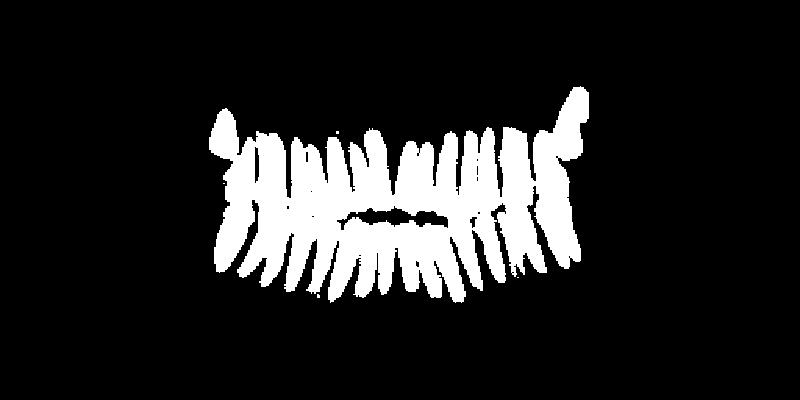
\includegraphics[width=8cm]{figures/maskintera.pdf}
    \caption{Maschera OPT binaria di partenza}
    \label{fig:maskintera}
\end{figure}
\begin{figure}[H]
    \centering
    \begin{minipage}{0.4\textwidth}
	\centering
    	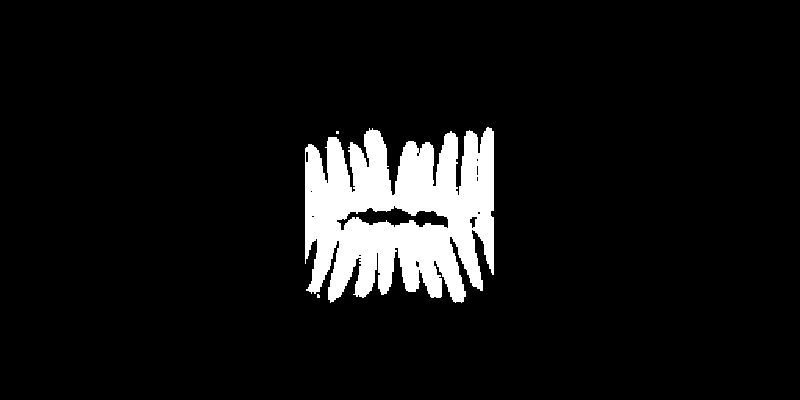
\includegraphics[width=8cm]{figures/maskfrontal.pdf}
    	\caption{Maschera bitewing frontale}
    	\label{lab:Maschera bitewing frontale}
    \end{minipage} \hfill
    \begin{minipage}{0.4\textwidth}
    	\centering
    	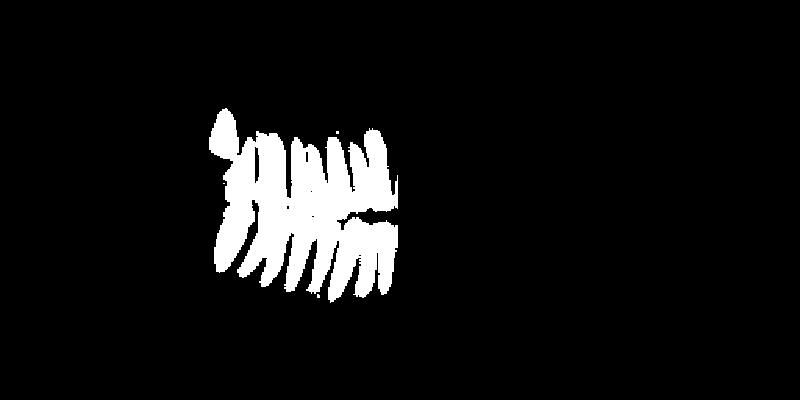
\includegraphics[width=8cm]{figures/masksx.pdf}
    	\caption{Maschera bitewing sinistro}
    	\label{lab:Maschera bitewing sinistro}
    \end{minipage}
\end{figure}
\begin{figure}[H]
    \centering
    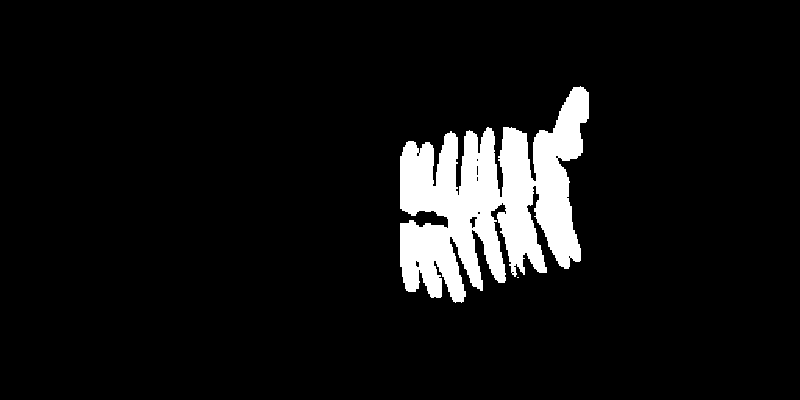
\includegraphics[width=8cm]{figures/maskdx.pdf}
    \caption{Maschera bitewing destro}
    \label{fig:Maschera bitewing destro}
\end{figure}
%Definizione di RoI più restrittive

Al termine di questo processamento, vengono a delinearsi 3 nuovi dataset, della stessa cardinalità del dataset delle ortopanoramiche, ciascuno contenente la corrispondente porzione della maschera.\\

A questo punto, viene definito un algoritmo di Feature Matching che utilizza queste nuove maschere binarie.\\
Viene, perciò, istanziato un oggetto SIFT, a partire dai metodi definiti nel punto precedente, ma a cui vengono forniti in input diverse versioni delle maschere binarie:
\begin{itemize}
\item Per l'interrogazione del dataset delle immagini frontali, viene fornito all'algoritmo, l'insieme delle maschere in cui è stata mantenuta unicamente l'area centrale della maschera originaria. Così facendo, l'area di identificazione dei keypoint per le immagini ortopanoramiche viene ristretta unicamente alla zona centrale. Il processo, dunque, sarà ancora più mirato e specifico rispetto al caso precedente. Infatti, tutti i punti esterni a quest'area, durante la fase di interrogazione delle immagini di bitewing frontali, possono essere considerati punti outlier.
\item  Per l'interrogazione, invece, del dataset contenente le immagini di bitewing laterale destro, viene fornito in input all'algoritmo l'insieme delle maschere in cui è stata mantenuta unicamente l'area laterale destra della maschera originaria. L'area di analisi dei keypoint per le immagini ortopanoramiche viene ristretta unicamente alla zona laterale destra; tutti i punti esterni a quest'area, durante la fase di interrogazione delle immagini di bitewing laterale destro, possono essere considerati punti outlier.
\item Similmente ai casi precedenti, per l'interrogazione del dataset delle immagini laterali sinistre, viene fornito all'algoritmo l'insieme delle maschere in cui è stata mantenuta unicamente l'area laterale sinistra della maschera originaria. Così facendo, l'area di identificazione dei keypoint per le immagini ortopanoramiche viene ristretta unicamente alla zona laterale sinistra e tutti i punti esterni a quest'area, possono essere considerati punti outlier.
\end{itemize}


%%%%%%%%%%%%%%%%%%%%%%%%%%%%%%%%%
\subsection{Valutazioni}
L'applicazione di questo algoritmo alle immagini ortopanoramiche, dovrebbe portare a risultati molto più accurati attraverso un'analisi mirata alle sole RoI:

\begin{figure}[H]
    \centering
    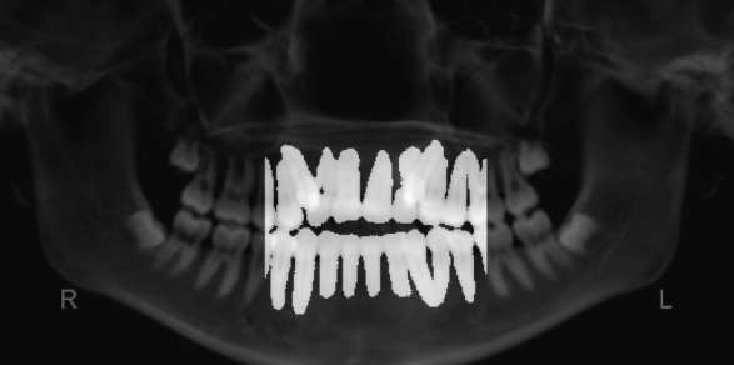
\includegraphics[width=8cm]{figures/optfrontal.pdf}
    \caption{Maschera OPT frontal}
    \label{fig:mascherafrontal}
\end{figure}
\begin{figure}[H]
    \centering
    \begin{minipage}{0.45\textwidth}
	\centering
    	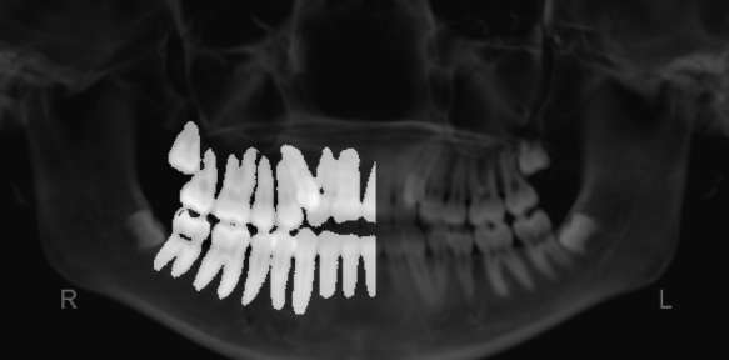
\includegraphics[width=8cm]{figures/optsx.pdf}
    	\caption{Maschera OPT sx}
    	\label{lab:Maschera sx}
    \end{minipage}\hfill
    \begin{minipage}{0.45\textwidth}
    	\centering
    	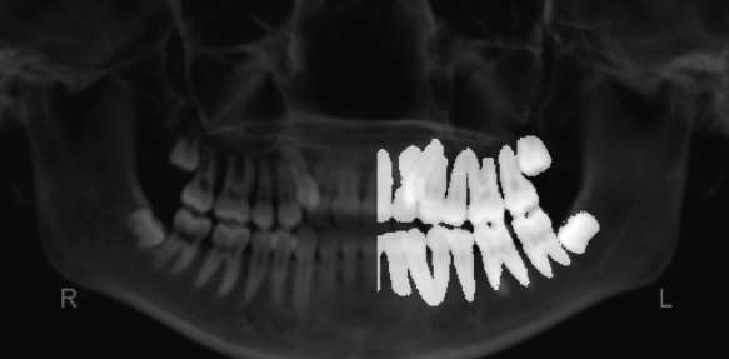
\includegraphics[width=8cm]{figures/optdx.pdf}
    	\caption{Maschera OPT dx}
    	\label{lab:Maschera dx}
    \end{minipage}\hfill
\end{figure}

Ma i risultati così ottenuti sono riportati di seguito:
\begin{figure}[H]
	\centering
	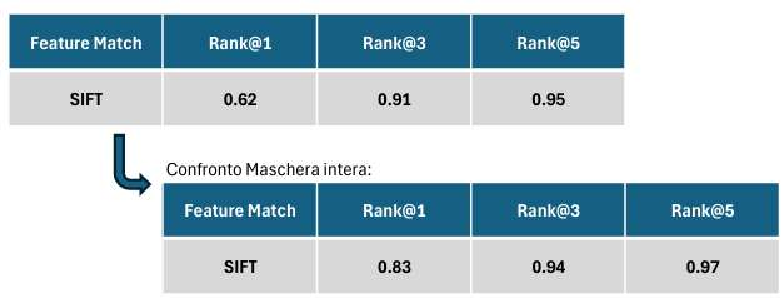
\includegraphics{figures/frontal3_1.pdf}
   	\caption{Accuracy Frontal Matching con RoI}
	\label{fig:frontal3}
\end{figure}
\begin{figure}[H]
	\centering
	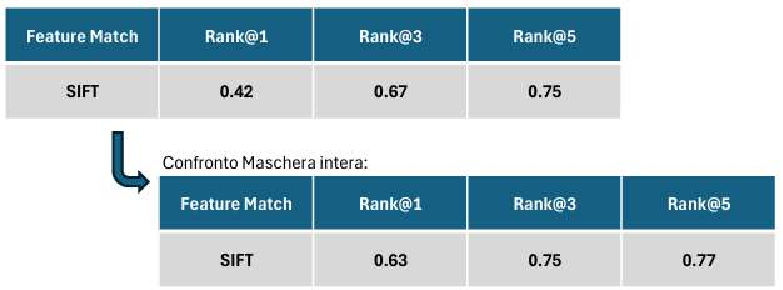
\includegraphics{figures/dx3_1.pdf}
    	\caption{Accuracy BTW DX Matching con RoI}
	\label{fig:dx3}
\end{figure}
\begin{figure}[H]
	\centering
	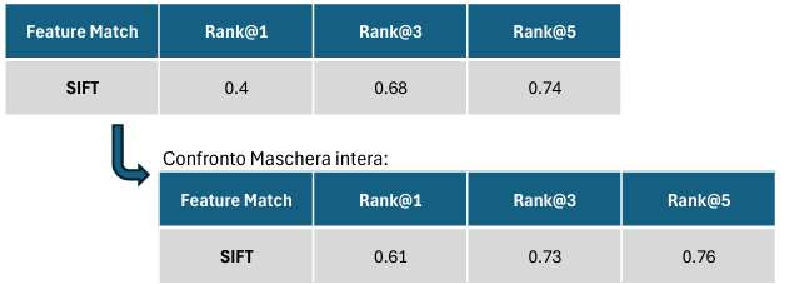
\includegraphics{figures/sx3_1.pdf}
    	\caption{Accuracy BTW SX Matching con RoI}
	\label{fig:sx3}
\end{figure}
\begin{figure}[H]
	\centering
	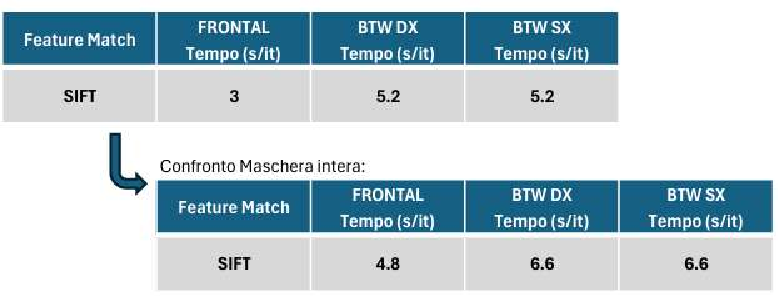
\includegraphics{figures/tempi3_1.pdf}
    	\caption{Tempi di esecuzione con definizione di RoI}
	\label{fig:tempi3}
\end{figure}

I valori di accuracy sono complessivamente diminuiti, a discapito dei tempi di processamento che sono stati, viceversa, ottimizzati.\\
Il problema dell'accuracy è legato all'algoritmo di generazione delle maschere. Come è possibile osservare dall'esempio sopra riportato, l'area di sovrapposizione della maschera binaria non ricopre interamente l'area che sarebbe da valutare; alcuni denti vengono esclusi e l'area di copertura del singolo detto è ristretta.\\
Nel seguito, verranno presentate delle ottimizzazioni atte a contrastare questi risultati non attesi.

%%%%%%%%%%%%%%%%%%%%%%%%%%%%%%%%%%%%%%%%%%%%%
\subsection{Problema del singolo match}
Finora, è stata valutata l'accuratezza nei modelli di matching a singola immagine di query. \\
E' però opportuno considerare anche il caso in cui il sistema possa essere utilizzato nella sua interezza. Infatti, una possibile futura applicazione potrebbe essere quella di fornire in input tutte e tre le immagini di bitewing e valutare così la combinazione dei singoli risultati al fine di individuare l'immagine di match con maggior valore di score totale.\\
Al fine di ottemperare questo obiettivo, è opportuno ideare un sistema che combini tutte e tre le precedenti valutazioni di match.

%%%%%%%%%%%%%%%%%%%%%%%%%%%%%%%%%%%%%%%%%%%%%
\chapter{Unione di match}
Un ulteriore utilizzo del sistema, è quello di effettuare la ricerca del miglior match, all'interno del dataset di ortopanoramiche, fornendo in ingresso le tre immagini di bitewing contemporaneamente. I risultati parziali di match, andranno quindi ad unirsi per produrre un risultato più consistente e completo.\\
A questo scopo, è stato definito un algoritmo che effettua la detta computazione.\\
E' stato realizzato perciò un sistema che, similmente al caso precedente, esegue il processo di Feature Matching per tutte le immagini di bitewing e, rispettivamente, restituisce un dictionary contenente, per ciascuna immagine, la lista dei migliori {\itshape n} match con relativi score.\\
La funzione per ottenere questo risultato, è {\itshape total\_matches}. Nel dettaglio:
\begin{itemize}
\item Viene effettuato il processo di estrazione delle feature e ricerca dei migliori match, per ogni immagine di query (laterale e frontale).
\item I risultati, vengono accumulati in un dictionary costituito da tante chiavi quante sono le immagini di query e, per ciascuna, memorizza una lista con i relativi migliori {\itshape n} match e i corrispondenti score.
\end{itemize}
Una volta ottenuti questi risultati, il cuore di questa fase del progetto, consiste nell'unire i risultati parziali, al fine di definire un risultato globale più completo e robusto.\\
Questo processo prevede diverse fasi:
\begin{enumerate}
\item \textbf{{\itshape def merge}}: fusione ordinata di tre liste di corrispondenze.
\begin{itemize}
\item In primo luogo, viene effettuato l'ordinamento dei 3 dictonary. Questa fase è fondamentale al fine di garantire che tutti e tre i dictionary abbiano le chiavi nello stesso ordine. L'idea, infatti, è quella di fornire in input, simultaneamente, 3 immagini parziali riferite alla stessa persona. Ordinandole, viene garantito che i diversi pazienti vengano valutati con tutte e tre le immagini parziali insieme.
\item Successivamente, viene effettuata l'unione dei risultati ottenuti. Si itera all'interno di un ciclo for sulla prima lista ordinata. Per ogni immagine, l'algoritmo concatena i corrispondenti dati di matches provenienti dalle tre liste (frontale, dx, sx) in corrispondenza dello stesso indice nella lista.
\item Si estrae il nome dell'immagine e si crea un nuovo identificativo concatenando la stringa "P\_" con il numero identificativo del paziente.
\item In output, viene resituita una lista sottoforma di dizionario, contenente tutti i dati relativi ai tre match, ragruppati e ordinati per paziente. 
\end{itemize}

\item \textbf{{\itshape def sum\_matches}}: somma e aggregazione delle corrispondenze.
\begin{itemize}

\begin{figure}[H]
	\centering
    	\lstinputlisting[language=Python,label={lst:unionofmatches}]{listings/summatches.py}
\end{figure} 

\item Viene presa in input la lista restituita dalla funzione definita nel punto precedente. Ogni lista si riferisce ai risultati di match ottenuti per ogni paziente.
\item Viene creato un dizionario in cui, in corrispondenza di ogni indice (immagine di match), viene valutata la lista di matches registrati. Se un'immagine è presente più di una volta, vengono sommati i relativi score e aggiornato il valore corrispondente a quello già esistente.
\item Al termine, il dizionario viene ordinato in base agli score dei matches ottenuti per ogni immagine, in ordine decrescente, e restituito come una lista di tuple.
\end{itemize}

\item A questo punto, viene valutata l'accuracy dei risultati ottenuti.
\begin{figure}[H]
	\centering
	\hspace{-1cm}
	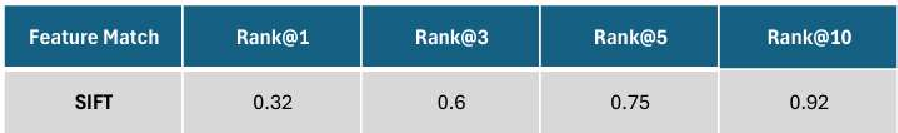
\includegraphics[width=17cm]{figures/3match.pdf}
    	\caption{Accuracy dell'unione dei 3 match}
	\label{fig:3matches}
\end{figure}
\end{enumerate}

Nei processi di fusione dei dati, è normale che l'accuratezza diminuisca dopo aver unito i risultati di match parziali, soprattutto se le corrispondenze provengono da fonti diverse (come nel caso delle diverse prospettive "frontal", "dx", "sx"). Una posibile valutazione potrebbe essere quella di ponderare i risultati ottenuti dai singoli match, considerando il fatto che i match calcolati per le immagini frontali sono più accurati rispetto a quelli laterali.


%%%%%%%%%%%%%%%%%%%%%%%%%%%%%%%%%%%%%%%%%%%%
\chapter{Ottimizzazioni}
I risultati ottenuti, dai vari step di processamento, non sono conformi con quanto atteso. All'aumentare del livello di precisione dell'algoritmo di matching, i risultati peggiorano in termini di accuracy, invece di migliorare grazie alla definizione di uno spazio di ricerca più accurato.\\
Questo fa presumere che ci sia un errore durante il processo di definizione dei diversi step.

%%%%%%%%%%%%%%%%%%%%%%%%%5
\section{Ottimizzazione algoritmo di Masking}

Analizzando, perciò, le maschere binarie generate dalla rete GAN, è possibile constatare come questa rete generativa non riesca a catturare, nella quasi totalità dei casi, la presenza di alcuni denti, in particolare, i "denti del giudizio". Inoltre, l'area individuata per ogni singolo dente, è molto stringente.\\
Questa mancanza causa errori di matching soprattutto durante le operazioni di interrogazione delle immagini di bitewing laterale.\\
Viene, perciò, definito un secondo algoritmo di masking.

%%%%%%%%%%%%%%%%%%%%%%%%%%%%%%%%%%%%%%%%%%
\subsection{U-Net Model}
Viene definita una nuova rete, secondo il modello \textbf{U-Net}.\\
\textbf{U-Net} è una rete neurale convoluzionale (CNN) progettata per compiti di Semantic Segmentation, particolarmente efficace in ambito medico. Nello specifico, è molto usata per segmentare immagini radiografiche, dove è importante identificare strutture anatomiche precise. \\
La rete U-Net nasce per compiti di segmentazione di immagini biomediche con una struttura "a U"; essa è composta da un percorso di contrazione e uno di espansione, che permettono di catturare sia i dettagli locali sia il contesto più ampio delle immagini.
\begin{figure}[H]
	\hspace{-2cm}
	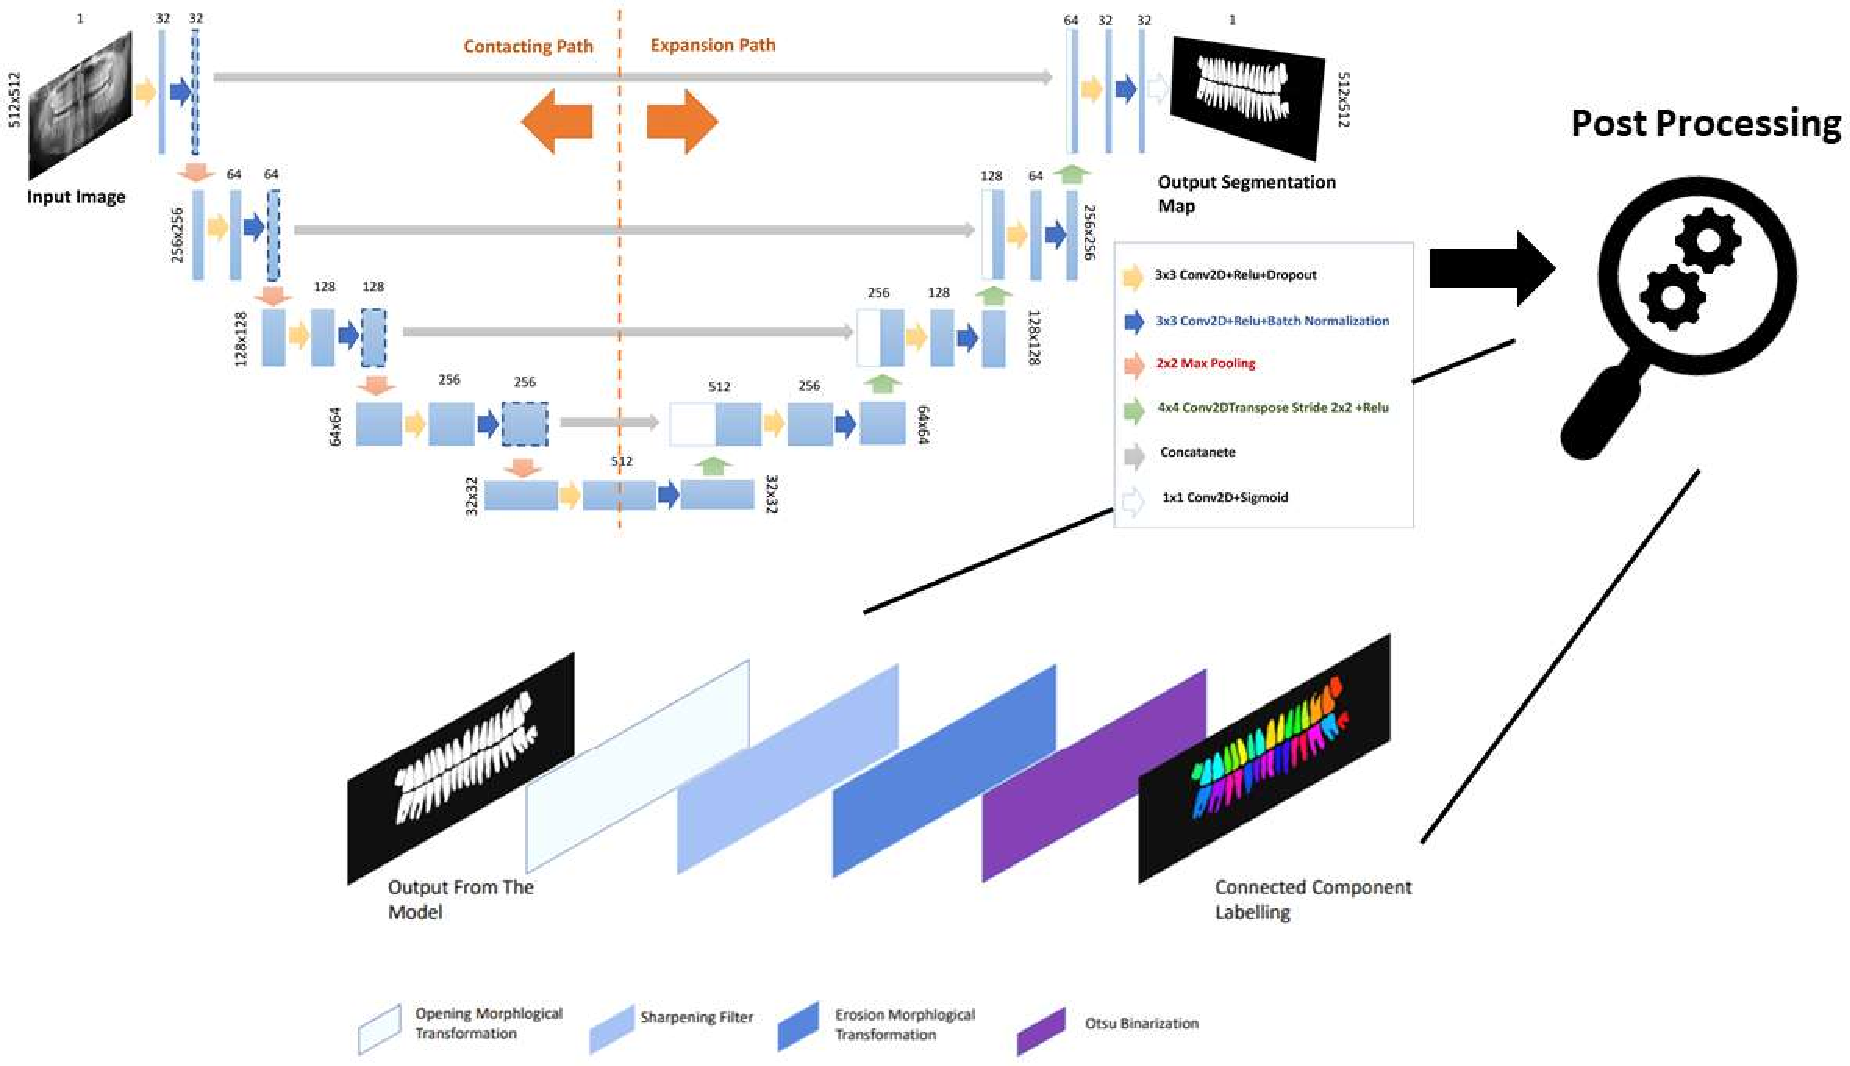
\includegraphics[height=10cm,width=18cm]{figures/ArchitectureUnet.pdf}
    	\caption{Architettura della rete U-Net}
	\label{fig:unet}
\end{figure}
Essa è caratterizzata, dunque, da due fasi principali:
\begin{enumerate}
\item \textbf{Encoder} (Contrazione): La parte sinistra della rete che si occupa di estrarre feature dell’immagine, riducendone progressivamente le dimensioni spaziali; contemporaneamente aumenta la profondità, permettendo alla rete di catturare caratteristiche complesse.
\item \textbf{Decoder} (Espansione): La parte destra della rete che espande le caratteristiche apprese, ripristinando la risoluzione spaziale originaria per produrre una mappa di segmentazione che corrisponde alle dimensioni dell’immagine iniziale. Utilizza anche operazioni di concatenazione (skip connections) con i livelli dell'encoder per preservare dettagli locali.
\end{enumerate}
L'algoritmo di definizione della maschere segue i seguenti passi implementativi principali:
\begin{enumerate}
\item \textbf{Definizione della U-Net}:
\begin{figure}[H]
    \centering
    \lstinputlisting[language=Python,label={lst:unetarchitecture}]{listings/unet.py}
\end{figure}

Viene definita una funzione UNET con dropout e batch normalization; essa è composta da:
\begin{itemize}
\item Encoder: la parte di compressione con livelli convoluzionali e pooling, al fine di catturare le feature dell'immagine.
\item Bottleneck: livello centrale per astrarre le feature principali.
\item Decoder: espande le feature al fine di ripristinare la dimensione originale, utilizza le skip connections, dal percorso encoder, con l'obiettivo di migliorare la segmentazione.
\end{itemize}

\item \textbf{Preprocessamento delle Immagini}:\\
La funzione {\itshape pre\_images} carica e ridimensiona le immagini. In particolare, converte l'immagine un unico canale poichè, alcune immagini, pur essendo in scala di grigi, possono essere valutate in 3 canali. Infine, ridimensiona e concatena le immagini. Tutte le immagini vengono ridimensionate a (512, 512), convertite in array e concatenate in un array tridimensionale.
\item \textbf{Incremento dei Dati con Albumentations}:\\
Sono applicati vari tipi di {\itshape Data Augmentation} sui dati (rotazione, ridimensionamento casuale, rumore gaussiano, sfocatura, e riflessione orizzontale) al fine di migliorare la generalizzazione del modello. Il processo viene ripetuto 4 volte con l'obiettivo di creare nuove varianti dei dati di addestramento, migliorando la robustezza del modello.
\item \textbf{Addestramento del Modello}:
Descrive la fase di compilazione e fit. Il modello viene compilato attraverso binary\_crossentropy e addestrato per 200 epoche, con un batch size di 8. Questo processo minimizza la perdita e ottimizza l'accuratezza su immagini binarie (denti o non denti).
\item \textbf{Predizione e Analisi}:
\begin{itemize}
\item Predizione della Maschera: \textbf{model.predict} genera le maschere segmentate per le immagini di test.
\item Sovrapposizione dei Contorni: \textbf{cv2.findContours}, individua i contorni della maschera predetta e li disegna sull'immagine originale al fine di visualizzare la segmentazione.
\end{itemize}
\item \textbf{Analisi CCA (Connected Component Analysis)}:\\
La funzione CCA\_Analysis viene utilizzata per l'analisi delle componenti connesse su immagini binarie; vengono contati i denti e segmentate le componenti connesse, identificando ogni dente in modo individuale.
\end{enumerate}

\textbf{Bottleneck}: Il livello centrale della rete U-Net funge da "collo di bottiglia", con lo scopo di concentrarsi sui tratti più distintivi e salienti dell’immagine.

%%%%%%%%%%%%%%%%%%%%%%%%%%%%%%%%%%%%%%%%%%55
\subsection{Metriche di Valutazione}
Dopo le fasi di training e di validation, l'algoritmo viene valutato e testato su un set di dati nuovi; le metriche così ottenute sono:
\begin{itemize}
\item Accuracy: 0.92
\item Loss: 0.03
\end{itemize}

Valori alti di Accuracy, insieme a valori bassi di loss, indicano che il modello si adatta bene ai dati.

%%%%%%%%%%%%%%%%%%%%%%%%%%%%%%%%%%%5
\subsection{Applicazione delle maschere}
L'algoritmo restituisce in output delle maschere che, rispetto alle precedenti, risultano più ampie e permissive, ricoprendo una zona più estesa dell'area dentale.
\begin{figure}[H]
    \centering
    \begin{minipage}{0.45\textwidth}
	\centering
    	\includegraphics[width=8cm]{figures/opt\_1\_first.pdf}
    	\caption{Primo Algoritmo di Masking}
    	\label{lab:Maschera 2 opt1}
    \end{minipage}\hfill
    \begin{minipage}{0.45\textwidth}
    	\centering
    	\includegraphics[width=8cm]{figures/opt\_1\_second.pdf}
    	\caption{Secondo Algoritmo di Masking}
    	\label{lab:Maschera 1 opt1}
    \end{minipage}\hfill
\end{figure}

Utilizzando questa nuova estrazione di maschere binarie possono essere ripetute le esecuzioni degli algoritmi definiti in precedenza.\\

\begin{itemize}
\item \textbf{Matching sull'intera Maschera}\\
Viene eseguito, in prima istanza, l'algoritmo SIFT per l'estrazione dei keypoint sulle immagini ortopanoramiche, con l'applicazione della nuova maschera binaria. Lo scopo, dunque, consiste nel delimitare la regione di interesse corrispondente all'intera arcata dentale. Il match, successivamente, verrà effettuato tra le immagini di bitewing fornite in input e i descrittori dei keypoint delle ortopanoramiche così definiti.\\
I risultati ottenuti sono riportati di seguito:
\begin{figure}[H]
	\centering
	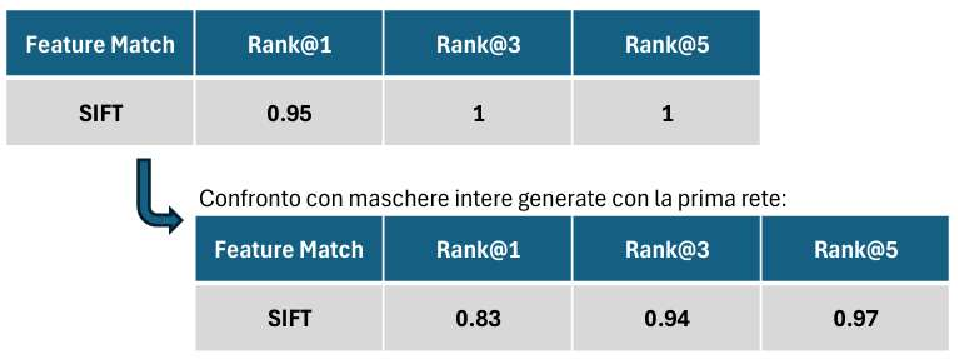
\includegraphics{figures/frontal4_1.pdf}
   	\caption{Accuracy Frontal Matching con U-Net}
	\label{fig:frontal4}
\end{figure}
\begin{figure}[H]
	\centering
	\includegraphics{figures/dx4_1.pdf}
    	\caption{Accuracy BTW DX Matching con U-Net}
	\label{fig:dx4}
\end{figure}
\begin{figure}[H]
	\centering
	\includegraphics{figures/sx4_1.pdf}
    	\caption{Accuracy BTW SX Matching con U-Net}
	\label{fig:sx4}
\end{figure}
\begin{figure}[H]
	\centering
	\includegraphics{figures/tempi4_1.pdf}
    	\caption{Tempi di esecuzione con U-Net}
	\label{fig:tempi4}
\end{figure}
Confrontando questi risultati con quelli ottenuti in precedenza per la stessa applicazione, ma attraverso un diverso algoritmo di generazione delle maschere, è possibile vedere chiaramente come questi risultati presentino valori di accuracy molto più elevati! A dimostrazione del fatto che la definizione dell'area di ricerca è il primo passo più importante nella realizzazione del progetto.

\item \textbf{Matching su una porzione della Maschera}\\
Viene ora rieseguito l'algoritmo di restringimento della RoI, che identifica una zona di match più precisa, individuando l'area della maschera corrispondente alla regione di interrogazione, rispettivamente per i match delle immagini di bitewing frontali e laterali (destra e sinistra).\\
I risultati ottenuti sono i seguenti:
\begin{figure}[H]
	\centering
	\includegraphics{figures/frontal5_1.pdf}
   	\caption{Accuracy Frontal Matching con RoI e U-Net}
	\label{fig:frontal5}
\end{figure}
\begin{figure}[H]
	\centering
	\includegraphics{figures/dx5_1.pdf}
    	\caption{Accuracy BTW DX Matching con RoI e U-Net}
	\label{fig:dx5}
\end{figure}
\begin{figure}[H]
	\centering
	\includegraphics{figures/sx5_1.pdf}
    	\caption{Accuracy BTW SX Matching con RoI e U-Net}
	\label{fig:sx5}
\end{figure}
\begin{figure}[H]
	\centering
	\includegraphics{figures/tempi5_1.pdf}
    	\caption{Tempi di esecuzione con RoI e U-Net}
	\label{fig:tempi5}
\end{figure}
\end{itemize}
I valori di accuracy sono migliorati rispetto all'esecuzione corrispondente nello studio precedente, soprattutto per il matching delle immagini frontali che è quasi perfetto già sui valori di Rank@1. Nonostante questo, però, i valori di accuracy con l'esecuzione di questo algoritmo peggiorano rispetto alla stessa valutazione effettuata attraverso l'intera maschera binaria applicata all'immagine ortopanoramica. Questo risultato non è conforme con quanto atteso, visto il raffinamento successivo; l'algoritmo dovrebbe risultare più preciso.

\subsection{Analisi degli errori di Match}
Si analizzano, perciò, gli errori di match riscontrati nell'esecuzione degli algoritmi di ricerca per le immagini di Bitewing laterali.\\
In figura vengono riportati alcuni errori di esecuzione dell'algoritmo SIFT:
\begin{figure}[H]
	\centering
	\includegraphics[width=13cm]{figures/matcherr.pdf}
   	\caption{Errore di Matching per BTW SX}
	\label{fig:matcherr}
\end{figure}
\begin{figure}[H]
	\centering
	\includegraphics[width=13cm]{figures/matcherr2.pdf}
    	\caption{Errore di Matching per BTW SX}
	\label{fig:matcherr2}
\end{figure}

Da queste immagini, evince che l'area di ricerca dei keypoint presenta alcuni errori e conseguentemente l'algoritmo di ricerca non risulta sempre corretto.

%%%%%%%%%%%%%%%%%%%%%%%%%%%%%%%%%%%%%%%%%
\section{Dilatazione delle Maschere}
In Computer Vision, i \textbf{keypoint} rappresentano punti di interesse significativi all'interno di un'immagine, spesso rappresentati come coordinate (x, y). Vengono utilizzati per descrivere e riconoscere le caratteristiche distintive di un'immagine, come bordi, angoli o altri dettagli salienti, che possono risultare utili al fine di identificare, tracciare o confrontare oggetti nelle immagini.\\

Il compito delle maschere è quello di delimitare le aree di ricerca. In questo progetto, delimitano le aree di ricerca alla sola arcata dentale. Ma è importante notare che i keypoint più significativi, per questo studio, si trovano proprio nei punti di giunzione tra due denti, come all'interno di bordi, nelle giunture mandibolari o nelle sovrapposizioni. Le maschere escludono queste specifiche zone, concentrandosi invece prettamente nell'area di occupazione del singolo dente.\\

Al fine di contrastare questo problema, la soluzione adottata è quella della \textbf{Dilatazione delle maschere}.
\begin{figure}[H]
    \centering
    \lstinputlisting[language=Python,label={lst:dilation}]{listings/dilation.py}
\end{figure}

Questo codice esegue un'operazione di dilatazione su un'immagine in scala di grigi, in particolare:
\begin{itemize}
\item \textbf{def dilatate\_mask}:\\
\begin{itemize}
\item Riceve in input un'immagine (la maschera) e una dimensione di dilatazione.
\item Crea un kernel (una matrice di valori pari a 1), della dimensione specificata, al fine di controllare la dilatazione.
\item Usa la funzione \textbf{cv2.dilate()} di OpenCV al fine di eseguire l'operazione di dilatazione sull'immagine; espande le aree chiare (i pixel con valori elevati) attorno ai bordi dell'oggetto.
\item Infine, restituisce in output l'immagine dilatata.
\end{itemize}
\item \textbf{def apply\_mask\_dilatated\_crop}:
\begin{itemize}
\item Legge l'immagine (maschera) in scala di grigi.
\item Passa l'immagine alla funzione {\itshape dilatate\_mask} al fine di ottenerne la versione dilatata.
\item Salva l'immagine dilatata nel percorso di output specificato.
\end{itemize}
\end{itemize}

L'operazione di dilatazione espande le aree di pixel chiari dell'immagine, al fine di:
\begin{itemize}
\item Riempire piccoli buchi nella maschera.
\item Connettere parti disgiunte di oggetti contigui.
\item Aumentare l'area di ricerca individuata dalla maschera, includendo aree di confine come i bordi.
\end{itemize}

Il risultato di questa operazione è un'immagine più ampia e conseguentemente un'area di ricerca maggiore.
\begin{figure}[H]
    \centering
    \begin{minipage}{0.45\textwidth}
	\centering
    	\includegraphics[width=8cm]{figures/OPT_8.pdf}
    	\caption{Maschera originale}
    	\label{lab:Maschera Originale}
    \end{minipage}\hfill
    \begin{minipage}{0.45\textwidth}
    	\centering
    	\includegraphics[width=8cm]{figures/OPT_8_mask.pdf}
    	\caption{Maschera dilatata}
    	\label{lab:Maschera dilatata}
    \end{minipage}\hfill
\end{figure}

Eseguendo l'algoritmo di matching con applicazione dell'intera maschera dilatata, i risultati di accuracy per le immagini di bitewing sinistro sono i seguenti:
\begin{figure}[H]
	\centering
	\includegraphics{figures/sx6_1.pdf}
    	\caption{Accuracy BTW SX Matching Dilated}
	\label{fig:sx6}
\end{figure}
Come è possibile osservare, i risultati sono peggiorati rispetto alla stessa valutazione effettuata su una maschera non dilatata.\\

Analizzando, però, nel dettaglio gli errori commessi dall'algoritmo, il peggioramento è dovuto all'amplificazione di aree bianche, non appartenenti realmente alla RoI. Infatti, in alcuni casi la rete U-Net utilzzata per l'estrazione delle maschere, identifica anche piccole aree, non appartenenti all'arcata dentale.\\
In seguito all'operazione di dilatazione, queste aree di outlier, risultanti da un errore prodotto dall'algoritmo di generazione delle maschere, vengono amplificate portando l'algoritmo SIFT a ricercare keypoint, e successivi match, in aree non appartenenti alla zona reale di interesse.\\
E' opportuno, allora, eliminare le aree di outlier al fine di incentrare l'elaborazione unicamente nell'area di interesse specificata.


%%%%%%%%%%%%%%%%%%%%%%%%%%%%%%%
\section{Post-processing delle maschere} 
Una rete UNet può occasionalmente catturare aree esterne vicine ai contorni della Regione di Interesse (RoI) a causa di challenges di precisione in corrispondenza dei bordi o a causa di leggeri sovrapposizioni nelle regioni segmentate.\\
E' possibile però implementare alcune soluzioni utili ad ignorare le aree esterne alla regione di interesse. Una di queste metodologie applica un'elaborazione di \textbf{Post-Processing} sulle maschere.\\
Il processo implementato segue due step principali, definiti, rispettivamente, dalle seguenti funzioni:
\begin{enumerate}
\item \textbf{post\_process\_mask}:
\begin{figure}[H]
    \centering
    \lstinputlisting[language=Python,label={lst:postprocessing}]{listings/postprocessing.py}
\end{figure}

La funzione effettua un'operazione di post-processing di una maschera binaria, al fine di rimuovere piccoli componenti di rumore ed eliminare gli oggetti che intersecano i bordi dell'immagine. In particolare, vengono effettate operazioni di:
\begin{itemize}
\item \textbf{Rimozione del Rumore attraverso l’Apertura Morfologica}:\\
Viene applicata un'operazione morfologica di {\itshape apertura} utilizzando un kernel ellittico di dimensioni (5, 5). Questo passaggio è utile al fine di rimuovere piccoli elementi di rumore isolati, mantenendo intatti i componenti a dimensionalità maggiore.
\item \textbf{Rimozione di Piccoli Componenti Connessi (Outliers):}\\
La funzione {\itshape connectedComponentsWithStats} individua tutti i componenti connessi (regioni continue di pixel bianchi) e calcola alcuni valori statistici, come l'area e le coordinate. Definisce un'area minima e crea una nuova maschera dove saranno conservati solo i componenti a dimensionalità sufficiente e che non si intersecano con i bordi dell'immagine. Viene iterato questo processo su ogni componente appartenente alla maschera individuato. I componenti che soddisfano entrambi i criteri vengono mantenuti nella maschera filtrata.
\item Infine, viene restituita la maschera filtrata, che rappresenta la versione post-elaborata della maschera iniziale, pulita dai piccoli componenti indesiderati e priva di regioni confinanti con i bordi.
\end{itemize}

Un esempio dei benefici introdotti dalla funzione, è visualizzabile di seguito: 
\begin{figure}[H]
    \centering
    \begin{minipage}{0.45\textwidth}
	\centering
    	\includegraphics[width=8cm]{figures/ds_2_img_19.pdf}
    	\caption{Maschera con imperfezioni}
    	\label{lab:Maschera imperfetta}
    \end{minipage}\hfill
    \begin{minipage}{0.45\textwidth}
    	\centering
    	\includegraphics[width=8cm]{figures/ds_2_img_19_mask.pdf}
    	\caption{Maschera con dropout degli outlier}
    	\label{lab:Maschera dropout}
    \end{minipage}\hfill
\end{figure}

\item Questo processamento è utile al fine di ottenere una maschera binaria pulita, in cui vengono eliminati i rumori e gli artefatti, mentre vengono mantenute solo le aree rilevanti. \\
Può però succedere, che alcune immagini presentino delle aree grigie erroneamente individuate al di fuori dell'arcata dentale e quindi non appartententi alla RoI. \\
Viene perciò implementata una funzione che sfrutta la \textbf{Connected Component Analysis}. Questa tecnica identifica le regioni grigie e le filtra in base alla presenza nella loro prossimità di aree bianche. 
\begin{enumerate}
\item \textbf{Connected Component Analysis}:\\
Identifica regioni continue nella maschera, classificandole come bianche, grigie o nere.
\item \textbf{Proximity Filtering}: \\
Per ogni regione grigia individuata, controlla se si sovrappone o è in prossimità di una regione bianca. Se è isolata, quindi non vicina ad una regione bianca, la rimuove settandola a nero.
\end{enumerate}
\begin{figure}[H]
    \centering
    \lstinputlisting[language=Python,label={lst:postprocessing2}]{listings/postprocessing2.py}
\end{figure}

\end{enumerate}

Eseguendo, ora, l'algoritmo di match sull'intera maschera così filtrata, è possibile osservare come i risultati di accuracy ottenuti siano nettamente migliorati, seppur ancora con margine di perfezionamento. \\
I risultati ottenuti sono i seguenti:
\begin{figure}[H]
	\centering
	\includegraphics{figures/sx7_1.pdf}
    	\caption{Accuracy Matching BTW SX con Post-Processing}
	\label{fig:sx6}
\end{figure}
I valori di accuracy sono ora molto migliorati, seppur ancora perfezionabili con ulteriori ottimizzazioni. \\
Gli errori di matching che possono essere osservati a questo punto, riguardano l'area di ricerca individuata dalla RoI. Vengono, perciò, applicate delle ottimizzazioni al processo di definizione delle RoI specifiche.

%%%%%%%%%%%%%%%%%%%%%%%%%%%%%%%%%%%%%%%%%%%
\section{Definizione della RoI con Coordinate}
L'algoritmo di restringimento delle RoI definito in precedenza funziona in generale, ma presenta alcune lacune.\\
Per arcate dentali complete, o che presentano la zona di interesse ricercata corrispondente all'immagine di bitewing di query, l'algoritmo delimita correttamente l'area di restringimento. %% c'era a capo 
Ma è importante evidenziare cosa succede quando queste condizioni non sono verificate. Di seguito viene mostrato un esempio:
\begin{figure}[H]
    \centering
    \begin{minipage}{0.45\textwidth}
	\centering
    	\includegraphics[width=8cm]{figures/mask\_26.pdf}
    	\caption{Maschera completa}
    	\label{lab:Maschera completa}
    \end{minipage}\hfill
    \begin{minipage}{0.45\textwidth}
    	\centering
    	\includegraphics[width=8cm]{figures/mask\_26\_crop.pdf}
    	\caption{Maschera con RoI SX}
    	\label{lab:Maschera con RoI sx}
    \end{minipage}\hfill
\end{figure}
 
L'esempio riportato, evidenzia chiaramente l'errore nella logica del calcolo. L'algoritmo, infatti, identifica all'interno della maschera le zone a tonalità bianca ed effettua un sezionamento dell'area, prelevando, in questo caso, solo una percentuale di quest'ultima, che si trova alla sua sinistra. In questo modo, però, \textbf{non considera la posizione spaziale} dell'area individuata. \\
Nella figura, si vede l'effetto prodotto: viene mantenuta la sezione sinistra dell'area individuata, che però si trova nell'area a destra dell'immagine.\\
L'algoritmo, in casi di maschere non complete o non contenenti l'area di interesse, non lavora correttamente; restituisce una maschera ridotta anche quando questa non dovrebbe essere restituita. Il motivo principale di questo errore, dunque, risiede nel fatto che l'algoritmo, così implementato, non considera in alcun modo le informazioni spaziali di collocamento dell'area bianca individuata.\\

Viene, perciò, definito un nuovo algoritmo ottimizzato per l'estrazione delle RoI considerando le dipendenze rispetto alla posizione occupata all'interno dell'immagine, e quindi alle coordinate.

\begin{figure}[H]
    \centering
    \lstinputlisting[language=Python,label={lst:sxRoI}]{listings/sxroi.py}
\end{figure}

La funzione \textbf{detect\_left\_white\_region} serve a individuare e restituire le coordinate del riquadro che delimita la regione bianca presente nella porzione sinistra di un'immagine di input.
\begin{itemize}
\item Viene estratta dalla maschera binaria l'area bianca identificativa dell'arcata dentale.
\item Viene calcolato il punto di delimitazione della porzione sinistra dell'arcata dentale, come coordinata x pari al 50\% della larghezza dell'intera immagine. Questo punto delimiterà la linea di separazione tra la parte sinistra e destra dell'immagine.
\item Viene effettuato il mascheramento della porzione destra, azzerando i pixel che appartengono all'area delimitata dalla coordinata x\_mid fino al bordo destro.
\item Viene mantenuta intatta solo la parte sinistra.
\item Vengono calcolate le nuove coordinate della maschera binaria sinistra e restituite in output.
\end{itemize}

L'algoritmo di Matching con SIFT così definito, è molto accurato. Viene implementato similmente anche per le valutazioni sulle immagini di bitewing destro e frontali. A tale scopo, sono state definite rispettivamente le funzioni:
\begin{itemize}
\item \textbf{detect\_right\_white\_region}:
\begin{itemize}
\item Simile alla logica analizzata precedentemente; il punto di divisione coincide sempre con il 50\% della larghezza dell'immagine.
\item Applica una maschera nella porzione sinistra rispetto al punto, impostando i valori a zero (nero), così da isolare e mantenere solo l'area a destra dell'immagine.
\item Calcola e ritorna le nuove coordinate dell'immagine di masking destro.
\end{itemize}

\item \textbf{detect\_frontal\_white\_region}:
\begin{itemize}
\item Calcola due punti di divisione. A partire dal punto medio rispetto alla larghezza dell'immagine, definisce i limiti x\_min e x\_max in modo tale che la regione centrale copra circa il 20\% della larghezza totale dell'immagine (± 10\% dal centro).
\item Imposta a zero (nero) le aree a sinistra di x\_min e a destra di x\_max nella maschera binaria, isolando, quindi, solo la regione centrale.
\item Determina le nuove coordinate della maschera a partire dai valori di x\_min e x\_max e li ritorna come output.
\end{itemize}
\end{itemize}

%I risultati di accuracy, ottenuti attraverso l'applicazione delle ottimizzazioni descritte, sono i seguenti:
%\begin{figure}[H]
%	\centering
%	\includegraphics{figures/sx8.pdf}
%    	\caption{Accuracy BTW SX Matching con coordinate}
%	\label{fig:sx8}
%\end{figure}
%Seppur migliorati, presentano ancora risultati non ottimi soprattutto in relazione ai valori di Rank@1.

%%%%%%%%%%%%%%%%%%%%%%%%%%%%%%%%%%%%%%%
\section{Modifica del Ratio test}
Dall'osservazione diretta dei match individuati, è possibile constatare come la maggior parte di essi appaiano molto vicini l'un l'altro e molto simili tra loro. Molti descrittori, infatti, vengono mappati nello stesso punto di match nell'immagine ortopanoramica corrispondente. Questo problema si manifesta a causa del valore selezionato per il Ratio Test. \\
Nel contesto del feature matching, il Ratio Test è applicato dopo aver individuato i keypoints, nelle due immagini, e aver calcolato i relativi descrittori. Durante il processo di matching, per ogni descrittore, appartenente ad una delle due immagini,  vengono individuati i descrittori più simili nella seconda immagine.\\
Questi descrittori simili, sono ordinati in base alla distanza euclidea; il più vicino, ossia il "miglior match", e il secondo più vicino come "secondo miglior match".\\
Il Ratio Test {\itshape confronta la distanza del miglior match con quella del secondo miglior match} e scarta i match in cui il rapporto tra queste distanze è superiore a una certa soglia (ad esempio 0.75).\\
E' necessario, perciò, definire il valore più accurato di questo parametro.\\
Per il dato studio, è opportuno diminuire il valore soglia definito, al fine di:
\begin{itemize}
\item \textbf{Ridurre il numero di falsi positivi}: Una soglia inferiore rende il test più selettivo, riducendo la probabilità di accettare corrispondenze deboli o errate, migliorando così la qualità complessiva dei match.
\item \textbf{Aumentare l'accuratezza del modello}: Nel contesto della Visione Artificiale, avere corrispondenze di qualità è fondamentale per la precisione di applicazioni come il feature matching.
\item \textbf{Migliorare la robustezza agli errori}: Una selezione più rigida dei match consente di ridurre l’impatto di rumore o variazioni di illuminazione, migliorando la robustezza del sistema.
\item \textbf{Efficienza computazionale}: Anche se può sembrare controintuitivo, un Ratio Test più basso porta spesso a meno match, riducendo i calcoli necessari per i passaggi successivi (come l'uso dell'algoritmo RANSAC, quando necessario).
\end{itemize}
Viene perciò decrementato il valore di Ratio Test a \textbf{0.7}.\\

Grazie a queste migliorie apportate, i valori di accuracy ottenuti attraverso l'algoritmo di matching per le immagini di bitewing SX sono i seguenti:
\begin{figure}[H]
	\centering
	\includegraphics{figures/sx9_1.pdf}
    	\caption{Accuracy BTW SX Matching Ottimizzato}
	\label{fig:sx9}
\end{figure}
I risultati di accuracy così ottenuti, sono complessivamente migliorati.
%%%%%%%%%%%%%%%%%%%%%%%%%%%%%%%%%%%%%%%
\section{Ottimizzazione maschere}
Immagini come quella sotto riportata presentano un livello di luminosità talmente elevato, da rendere difficile l'individuazione dei singoli denti anche all'occhio umano. \\
L'algoritmo di generazione delle maschere, in casi come questo, non è in grado di estrarre correttamente l'immagine binaria corrispondente.
\begin{figure}[H]
	\centering
	\includegraphics[width=12cm]{figures/ds\_6\_img\_176.pdf}
    	\caption{Luminosità Elevata}
	\label{fig:luminosità}
\end{figure}
\begin{figure}[H]
	\centering
	\includegraphics[width=12cm]{figures/ds\_6\_img\_176_mask.pdf}
    	\caption{Maschera corrispondente}
	\label{fig:maskLuminosa}
\end{figure}
Viene, perciò, definita un'opportuna funzione di \textbf{Pre-processing} da applicare alle immagini ortopanoramiche, prima di essere fornite in input alla rete di generazione delle maschere.\\
Questa funzione, {\itshape uniform\_luminosity\_contrast}, ha l'obiettivo di migliorare il contrasto e uniformare la luminosità di un'immagine, attraverso l'implementazione di un'opportuna trasformazione nello \textbf{spazio colore LAB} e attraverso l'ausilio della tecnica \textbf{CLAHE} (Contrast Limited Adaptive Histogram Equalization) sul canale di luminosità L.
\begin{figure}[H]
    \centering
    \lstinputlisting[language=Python,label={lst:luminosity}]{listings/luminosity.py}
\end{figure}
Vengono implementati i seguenti passaggi:
\begin{enumerate}
\item \textbf{Conversione allo Spazio Colore LAB}:\\
Viene convertita l’immagine nello spazio colore LAB (L: Luminosità, A: Verde-Rosso, B: Blu-Giallo). Questo spazio colore è utile ai fini della manipolazione della luminosità; in questo modo, le informazioni di contrasto e di luminosità possono essere regolate più facilmente attraverso la separazione del canale L.
\item \textbf{Separazione dei Canali}:\\
Viene effettuata la divisione dell’immagine LAB nei singoli canali L, A, e B. 
\begin{itemize}
\item Il canale L rappresenta le informazioni di luminosità dell’immagine.
\item Viceversa, i canali A e B gestiscono le informazioni cromatiche.
\end{itemize}
\item \textbf{Creazione e Applicazione di CLAHE sul Canale L}:\\
CLAHE viene creato con un {\itshape clipLimit} di 1.0 e una {\itshape tileGridSize} di 8×8. L'obiettivo dell'applicazione di CLAHE è migliorare il contrasto, limitando il clipping, e suddividendo l'immagine in piccole aree, che uniformano l'istogramma e riducono l'effetto di sovraesposizione.
\item \textbf{Calcolo e Regolazione della Luminosità Attuale}:\\
Viene determinata la luminosità media attuale del canale L (attraverso {\itshape .mean()}). Viene, poi, regolato il livello di luminosità scalando il canale L al fine di avvicinarsi alla luminosità target definita ({\itshape target\_luminosity}).Viene utilizzata la funzione {\itshape cv2.normalize} per mappare i valori del canale L all’ interno dell'intervallo specificato, centrato attorno alla luminosità target. Questa operazione mantiene il contrasto all'interno del canale di luminosità.
\item \textbf{Applicazione ulteriore di CLAHE}:\\
Viene applicata CLAHE sul canale L, normalizzato, al fine di migliorare ulteriormente il contrasto e garantire un aspetto uniforme.
\item \textbf{Ricombinazione dei Canali e Conversione a BGR}:\\
Vengono riuniti i canali L, A e B, ricostruendo, così, l’immagine LAB. Viene, infine, convertita l’immagine LAB pre-elaborata, nello spazio colore BGR per riportarla allo spazio colore originale e renderla visualizzabile in RGB.
\end{enumerate}

\begin{figure}[H]
	\centering
	\includegraphics[width=12cm]{figures/ds\_6\_img\_176_mask_2.pdf}
    	\caption{Maschera corrispondente}
	\label{fig:maskLuminosa}
\end{figure}
Grazie al pre-processing delle immagini ortopanoramiche vengono contrastati gli errori di generazione delle maschere binarie in casi limite.
Infatti, la maschera corrispondente all'esempio precedente, ora risulta perfettamente definita.

%%%%%%%%%%%%%%%%%%%%%%%%%%%%%%%5
\section{Risultati ottenuti}
I risultati che ora vengono presentati, sono il prodotto dell'applicazione e combinazione di tutti i processi di ottimizzazione precedentemente descritti. Anche l'ordine di applicazione è molto importante al fine del raggiungimento dei massimi risultati. Vengono, perciò, realizzati i seguenti passi computazionali:
\begin{enumerate}
\item \textbf{Pre-processing delle immagini ortopanoramiche}: al fine di migliorare il contrasto e uniformare la luminosità delle immagini. I valori che vengono impostati sono: {\itshape target\_luminosity=50}, {\itshape clipLimit=1.0}, {\itshape titleGridSize=(8,8)}.
\item \textbf{Estrazione delle maschere binarie}: attraverso l'esecuzione della seconda rete neurale, la rete U-Net.
\item \textbf{Post-processing delle maschere}: al fine di eliminare le aree erroneamente catturate durante il processo di generazione delle maschere. Viene prima eseguita la funzione {\itshape post\_process\_mask} e successivamente, la funzione {\itshape remove\_isolated\_gray\_regions}.
\item \textbf{Dilatazione delle maschere}: al fine di catturare keypoint significativi, come bordi e zone di confine. Viene impostato un valori di {\itshape dilation\_size} pari a 20.
\item \textbf{Definizione delle RoI attraverso i valori di coordinate}: rispettivamente, per le immagini di bitewing sinistro, destro e frontali. Per le prime due, viene definito {\itshape x\_mid = width //2} e considerata rispettivamente la parte a sinistra e a destra rispetto tale punto, mentre per la terza tipologia di immagini, viene considerato il 20\% della larghezza dell'immagine, centrato in x\_mid.
\item \textbf{Esecuzione dell'algoritmo SIFT}: con valori di {\itshape Lowe's Ratio Test} pari a 0.7.
\end{enumerate}
I risultati così ottenuti, sono confrontati con quelli prodotti dall'applicazione dell'algoritmo SIFT, con il medesimo valore di Lowe's test, sul dataset delle 2309 immagini ortopanoramiche, senza ausilio di nessun tipo di ottimizzazione.
\begin{figure}[H]
	\centering
	\includegraphics{figures/frontal6_1.pdf}
    	\caption{Accuracy Frontal Matching Ottimizzato}
	\label{fig:frontalopt}
\end{figure}
\begin{figure}[H]
	\centering
	\includegraphics{figures/dx6_1.pdf}
    	\caption{Accuracy BTW dx Matching Ottimizzato}
	\label{fig:dxopt}
\end{figure}+\begin{figure}[H]
	\centering
	\includegraphics{figures/sx10_1.pdf}
    	\caption{Accuracy BTW sx Matching Ottimizzato}
	\label{fig:sxopt}
\end{figure}
\begin{figure}[H]
	\centering
	\includegraphics{figures/tempi6_1.pdf}
    	\caption{Tempi Matching Ottimizzato}
	\label{fig:tempiopt}
\end{figure}

A questo punto, è possibile anche effettuare un'ulteriore valutazione. Precedentemente, a causa della struttura imperfetta degli algoritmi, l'algoritmo di Unione dei 3 match ha portato a risultati di accuracy molto bassi. Questo problema era dovuto alla non ottimalità dei 3 diversi algoritmi che, una volta uniti, ha peggiorato ulteriormente la computazione.\\
In seguito alle ottimizzazioni introdotte e al raggiungimento di risultati molto buoni da parte degli algoritmi definiti, è possibile rieseguire l'algoritmo di unione di match, considerando, però, le ultime valutazioni presentate.\\
Perciò, eseguendo l'algoritmo di unione di match, attraverso i passi computazionali definiti in questa sezione, i risultati di accuracy sono sorprendenti:
\begin{figure}[H]
	\centering
	\includegraphics[width=16cm]{figures/3match_1.pdf}
    	\caption{Accuracy Unione di Match Ottimizzato}
	\label{fig:unioneopt}
\end{figure}

%%%%%%%%%%%%%%%%%%%%%%%%%%%%%%%%%%%%%%%
\chapter{Conclusioni}


%%%%%%%%%%%%%%%%%%%%%%%%%%%%%%%%%%%%%%%
%\chapter{Contribution}
%I suggest referencing stuff as follows: \cref{fig:random-image} or \Cref{fig:random-image}
%
%You may also put some code snippet (which is NOT float by default), eg: \cref{lst:random-code}.
%
%\lstinputlisting[float,language=Java,label={lst:random-code}]{listings/HelloWorld.java}
%
%\section{Fancy formulas here}

%----------------------------------------------------------------------------------------
% BIBLIOGRAPHY
%----------------------------------------------------------------------------------------

\backmatter

\nocite{*} % Remove this as soon as you have the first citation

\bibliographystyle{alpha}
\bibliography{bibliography}

\begin{acknowledgements} % this is optional
Optional. Max 1 page.
\end{acknowledgements}

\end{document}
